% Options for packages loaded elsewhere
\PassOptionsToPackage{unicode}{hyperref}
\PassOptionsToPackage{hyphens}{url}
%
\documentclass[
]{book}
\usepackage{amsmath,amssymb}
\usepackage{lmodern}
\usepackage{iftex}
\ifPDFTeX
  \usepackage[T1]{fontenc}
  \usepackage[utf8]{inputenc}
  \usepackage{textcomp} % provide euro and other symbols
\else % if luatex or xetex
  \usepackage{unicode-math}
  \defaultfontfeatures{Scale=MatchLowercase}
  \defaultfontfeatures[\rmfamily]{Ligatures=TeX,Scale=1}
\fi
% Use upquote if available, for straight quotes in verbatim environments
\IfFileExists{upquote.sty}{\usepackage{upquote}}{}
\IfFileExists{microtype.sty}{% use microtype if available
  \usepackage[]{microtype}
  \UseMicrotypeSet[protrusion]{basicmath} % disable protrusion for tt fonts
}{}
\makeatletter
\@ifundefined{KOMAClassName}{% if non-KOMA class
  \IfFileExists{parskip.sty}{%
    \usepackage{parskip}
  }{% else
    \setlength{\parindent}{0pt}
    \setlength{\parskip}{6pt plus 2pt minus 1pt}}
}{% if KOMA class
  \KOMAoptions{parskip=half}}
\makeatother
\usepackage{xcolor}
\usepackage{color}
\usepackage{fancyvrb}
\newcommand{\VerbBar}{|}
\newcommand{\VERB}{\Verb[commandchars=\\\{\}]}
\DefineVerbatimEnvironment{Highlighting}{Verbatim}{commandchars=\\\{\}}
% Add ',fontsize=\small' for more characters per line
\usepackage{framed}
\definecolor{shadecolor}{RGB}{248,248,248}
\newenvironment{Shaded}{\begin{snugshade}}{\end{snugshade}}
\newcommand{\AlertTok}[1]{\textcolor[rgb]{0.94,0.16,0.16}{#1}}
\newcommand{\AnnotationTok}[1]{\textcolor[rgb]{0.56,0.35,0.01}{\textbf{\textit{#1}}}}
\newcommand{\AttributeTok}[1]{\textcolor[rgb]{0.77,0.63,0.00}{#1}}
\newcommand{\BaseNTok}[1]{\textcolor[rgb]{0.00,0.00,0.81}{#1}}
\newcommand{\BuiltInTok}[1]{#1}
\newcommand{\CharTok}[1]{\textcolor[rgb]{0.31,0.60,0.02}{#1}}
\newcommand{\CommentTok}[1]{\textcolor[rgb]{0.56,0.35,0.01}{\textit{#1}}}
\newcommand{\CommentVarTok}[1]{\textcolor[rgb]{0.56,0.35,0.01}{\textbf{\textit{#1}}}}
\newcommand{\ConstantTok}[1]{\textcolor[rgb]{0.00,0.00,0.00}{#1}}
\newcommand{\ControlFlowTok}[1]{\textcolor[rgb]{0.13,0.29,0.53}{\textbf{#1}}}
\newcommand{\DataTypeTok}[1]{\textcolor[rgb]{0.13,0.29,0.53}{#1}}
\newcommand{\DecValTok}[1]{\textcolor[rgb]{0.00,0.00,0.81}{#1}}
\newcommand{\DocumentationTok}[1]{\textcolor[rgb]{0.56,0.35,0.01}{\textbf{\textit{#1}}}}
\newcommand{\ErrorTok}[1]{\textcolor[rgb]{0.64,0.00,0.00}{\textbf{#1}}}
\newcommand{\ExtensionTok}[1]{#1}
\newcommand{\FloatTok}[1]{\textcolor[rgb]{0.00,0.00,0.81}{#1}}
\newcommand{\FunctionTok}[1]{\textcolor[rgb]{0.00,0.00,0.00}{#1}}
\newcommand{\ImportTok}[1]{#1}
\newcommand{\InformationTok}[1]{\textcolor[rgb]{0.56,0.35,0.01}{\textbf{\textit{#1}}}}
\newcommand{\KeywordTok}[1]{\textcolor[rgb]{0.13,0.29,0.53}{\textbf{#1}}}
\newcommand{\NormalTok}[1]{#1}
\newcommand{\OperatorTok}[1]{\textcolor[rgb]{0.81,0.36,0.00}{\textbf{#1}}}
\newcommand{\OtherTok}[1]{\textcolor[rgb]{0.56,0.35,0.01}{#1}}
\newcommand{\PreprocessorTok}[1]{\textcolor[rgb]{0.56,0.35,0.01}{\textit{#1}}}
\newcommand{\RegionMarkerTok}[1]{#1}
\newcommand{\SpecialCharTok}[1]{\textcolor[rgb]{0.00,0.00,0.00}{#1}}
\newcommand{\SpecialStringTok}[1]{\textcolor[rgb]{0.31,0.60,0.02}{#1}}
\newcommand{\StringTok}[1]{\textcolor[rgb]{0.31,0.60,0.02}{#1}}
\newcommand{\VariableTok}[1]{\textcolor[rgb]{0.00,0.00,0.00}{#1}}
\newcommand{\VerbatimStringTok}[1]{\textcolor[rgb]{0.31,0.60,0.02}{#1}}
\newcommand{\WarningTok}[1]{\textcolor[rgb]{0.56,0.35,0.01}{\textbf{\textit{#1}}}}
\usepackage{longtable,booktabs,array}
\usepackage{calc} % for calculating minipage widths
% Correct order of tables after \paragraph or \subparagraph
\usepackage{etoolbox}
\makeatletter
\patchcmd\longtable{\par}{\if@noskipsec\mbox{}\fi\par}{}{}
\makeatother
% Allow footnotes in longtable head/foot
\IfFileExists{footnotehyper.sty}{\usepackage{footnotehyper}}{\usepackage{footnote}}
\makesavenoteenv{longtable}
\usepackage{graphicx}
\makeatletter
\def\maxwidth{\ifdim\Gin@nat@width>\linewidth\linewidth\else\Gin@nat@width\fi}
\def\maxheight{\ifdim\Gin@nat@height>\textheight\textheight\else\Gin@nat@height\fi}
\makeatother
% Scale images if necessary, so that they will not overflow the page
% margins by default, and it is still possible to overwrite the defaults
% using explicit options in \includegraphics[width, height, ...]{}
\setkeys{Gin}{width=\maxwidth,height=\maxheight,keepaspectratio}
% Set default figure placement to htbp
\makeatletter
\def\fps@figure{htbp}
\makeatother
\setlength{\emergencystretch}{3em} % prevent overfull lines
\providecommand{\tightlist}{%
  \setlength{\itemsep}{0pt}\setlength{\parskip}{0pt}}
\setcounter{secnumdepth}{5}
\usepackage{booktabs}
\usepackage{booktabs}
\usepackage{longtable}
\usepackage{array}
\usepackage{multirow}
\usepackage{wrapfig}
\PassOptionsToPackage{x11names}{xcolor}
\usepackage{float}
\usepackage{colortbl}
\usepackage{pdflscape}
\usepackage{tabu}
\usepackage{threeparttable}
\usepackage{threeparttablex}
\usepackage[normalem]{ulem}
\usepackage{makecell}
\usepackage{graphicx}
\usepackage{fancyhdr}
%\usepackage[ngerman]{babel}

%%%%%%%%The footer on every page
\pagestyle{fancy}
\fancyfoot{\centering\footnotesize\upshape We reserve all rights in this document and in the information contained therein.  Reproduction, use or disclosure to third parties without express authority is strictly forbidden. * 2018 ABB Schweiz AG}
\pagestyle{headings}

%%%%%%%%%Slect the font you want to use
%http://www.tug.dk/FontCatalogue/montserratlight/
%\usepackage[defaultfam,light,tabular,lining]{montserrat} %% Option 'defaultfam'
%% only if the base font of the document is to be sans serig
%\usepackage[T1]{fontenc}
%\renewcommand*\oldstylenums[1]{{\fontfamily{Montserrat-TOsF}\selectfont #1}}

%%%%%%%%The custom rmdnote, rmdinfo etc parts of the pdf.
\makeatletter
\newenvironment{kframe}{%
\medskip{}
\setlength{\fboxsep}{.8em}
 \def\at@end@of@kframe{}%
 \ifinner\ifhmode%
  \def\at@end@of@kframe{\end{minipage}}%
  \begin{minipage}{\columnwidth}%
 \fi\fi%
 \def\FrameCommand##1{\hskip\@totalleftmargin \hskip-\fboxsep
 \colorbox{shadecolor}{##1}\hskip-\fboxsep
     % There is no \\@totalrightmargin, so:
     \hskip-\linewidth \hskip-\@totalleftmargin \hskip\columnwidth}%
 \MakeFramed {\advance\hsize-\width
   \@totalleftmargin\z@ \linewidth\hsize
   \@setminipage}}%
 {\par\unskip\endMakeFramed%
 \at@end@of@kframe}
\makeatother

\makeatletter
\@ifundefined{Shaded}{
}{\renewenvironment{Shaded}{\begin{kframe}}{\end{kframe}}}
\makeatother

\newenvironment{rmdblock}[1]
  {
  \begin{itemize}
  \renewcommand{\labelitemi}{
    \raisebox{-.7\height}[0pt][0pt]{
      {\setkeys{Gin}{width=3em,keepaspectratio}\includegraphics{images/#1}}
    }
  }
  \setlength{\fboxsep}{1em}
  \begin{kframe}
  \item
  }
  {
  \end{kframe}
  \end{itemize}
  }
\newenvironment{rmdnote}
  {\begin{rmdblock}{note}}
  {\end{rmdblock}}
\newenvironment{rmdcaution}
  {\begin{rmdblock}{caution}}
  {\end{rmdblock}}
\newenvironment{rmdimportant}
  {\begin{rmdblock}{important}}
  {\end{rmdblock}}
\newenvironment{rmdtip}
  {\begin{rmdblock}{tip}}
  {\end{rmdblock}}
\newenvironment{rmdwarning}
  {\begin{rmdblock}{warning}}
  {\end{rmdblock}}
\ifLuaTeX
  \usepackage{selnolig}  % disable illegal ligatures
\fi
\usepackage[]{natbib}
\bibliographystyle{apalike}
\IfFileExists{bookmark.sty}{\usepackage{bookmark}}{\usepackage{hyperref}}
\IfFileExists{xurl.sty}{\usepackage{xurl}}{} % add URL line breaks if available
\urlstyle{same} % disable monospaced font for URLs
\hypersetup{
  pdftitle={R Tutorial Example},
  pdfauthor={CONAPO},
  hidelinks,
  pdfcreator={LaTeX via pandoc}}

\title{R Tutorial Example}
\author{CONAPO}
\date{2022-09-29}

\begin{document}
\maketitle

{
\setcounter{tocdepth}{1}
\tableofcontents
}
\hypertarget{introducciuxf3n}{%
\chapter{Introducción}\label{introducciuxf3n}}

En este ejercicio se empieza con utilizar archivos \texttt{.Rmd} y cada archivo \texttt{RMarkdown} puede contener un capítulo o varios encabezados dependiendo del tema.

\textbf{Tutorial de Bookdown}

\href{https://bookdown.org/yihui/bookdown/}{\texttt{bookdown:\ Authoring\ Books\ and\ Technical\ Documents\ with\ R\ Markdown}} o bien citando al autor \citet{bookdown2016}

\hypertarget{rmarkdown}{%
\section{RMarkdown}\label{rmarkdown}}

\href{https://bookdown.org/yihui/rmarkdown/}{\texttt{R\ Markdown:\ The\ Definitive\ Guide}}
\href{https://www.rstudio.com/wp-content/uploads/2015/03/rmarkdown-reference.pdf}{\texttt{R\ Markdown:\ Reference\ Guide}}

En RStudio, se puede crear un nuevo archivo \texttt{.Rmd} desde el menú \texttt{File\ -\textgreater{}\ New\ File\ -\textgreater{}\ R\ Markdown}.

Hay tres componentes básicos de un documento RMarkdown: los metadatos, el texto y el código.

\begin{itemize}
\tightlist
\item
  Sintax de los metadatos conocido como: \texttt{YALM}. Donde este tipo de formato es imporante conservar la sangría dentro del YAML y también es importante que todos los subcampos esten en el lugar correcto. Sino enviará error a la hora de exportar los archivos.
\end{itemize}

\textbf{YAML}

\begin{Shaded}
\begin{Highlighting}[]
\PreprocessorTok{{-}{-}{-}}
\FunctionTok{title}\KeywordTok{:}\AttributeTok{ }\StringTok{"Hello R Markdown"}
\FunctionTok{author}\KeywordTok{:}\AttributeTok{ }\StringTok{"Awesome Me"}
\FunctionTok{date}\KeywordTok{:}\AttributeTok{ }\StringTok{"2018{-}02{-}14"}
\FunctionTok{output}\KeywordTok{:}\AttributeTok{ html\_document}
\PreprocessorTok{{-}{-}{-}}
\end{Highlighting}
\end{Shaded}

\textbf{Chunk}

Un fragmento de código comienza con tres acentos ``backticks'' como \texttt{\textasciigrave{}\textasciigrave{}\textasciigrave{}\{r\}} donde \texttt{r} indica el nombre del idioma, y termina con tres acentos.

\begin{itemize}
\item
  También se puede escribir opciones de fragmentos entre llaves (por ejemplo, establecer la altura de la figura en 5 pulgadas: \texttt{\textasciigrave{}\textasciigrave{}\textasciigrave{}\{r,\ fig.height=5\}}).
\item
  Una expresión de código \texttt{R} en línea comienza \texttt{\textasciigrave{}r} termina con un acento \texttt{\textasciigrave{}}.
\end{itemize}

\hypertarget{knitr}{%
\section{Knitr}\label{knitr}}

\href{https://yihui.org/knitr/}{Elegant, flexible, and fast dynamic report generation with R}

\begin{verbatim}
## Loading required package: knitr
\end{verbatim}

\begin{verbatim}
## Warning: package 'knitr' was built under R version 4.2.1
\end{verbatim}

\begin{verbatim}
## Loading required package: rmarkdown
\end{verbatim}

\begin{verbatim}
## Warning: package 'rmarkdown' was built under R version 4.2.1
\end{verbatim}

\begin{figure}
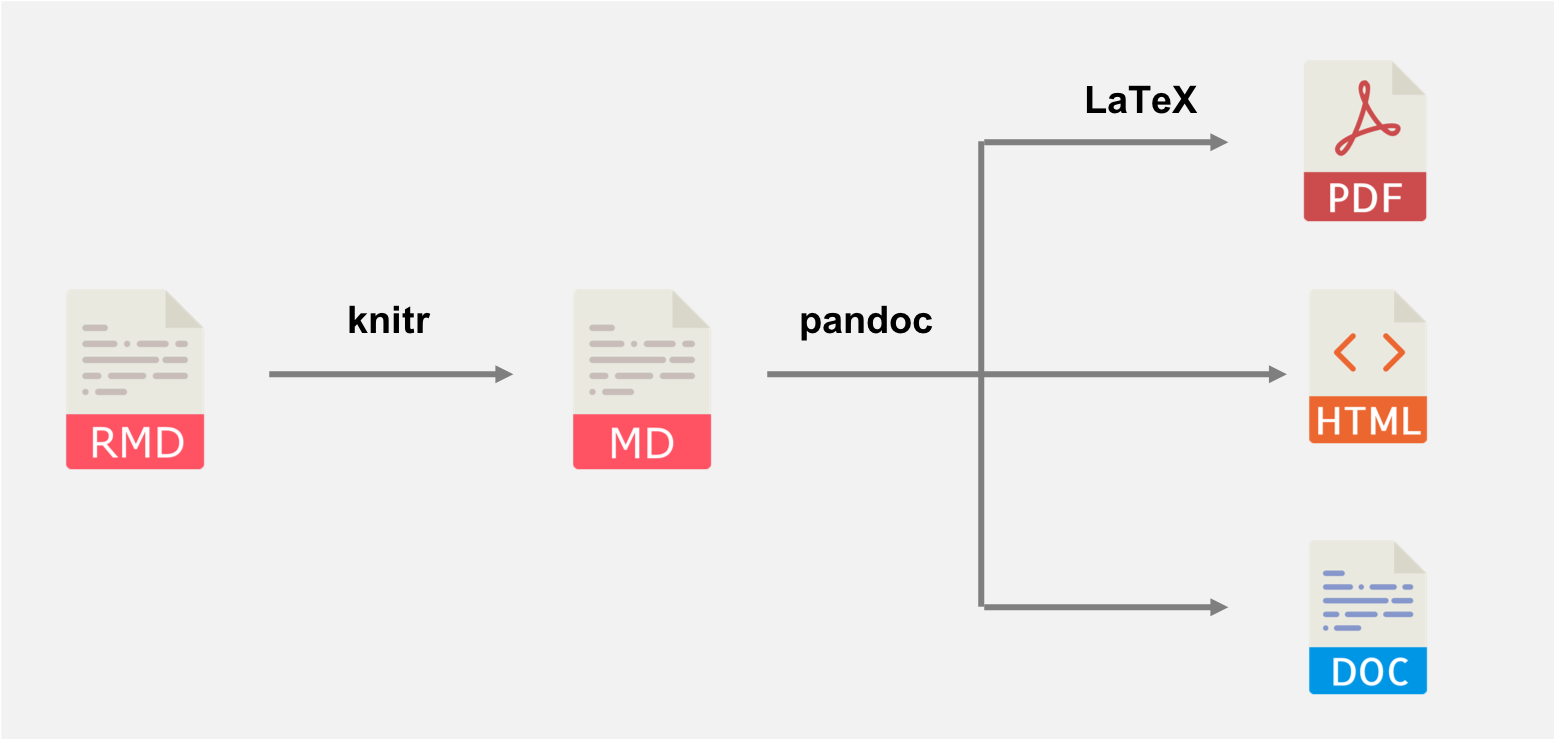
\includegraphics[width=1\linewidth]{images/workflow} \caption{A diagram illustrating how an R Markdown document is converted to the final output document.}\label{fig:rmdworkflow}
\end{figure}

La forma habitual de compilar un documento R Markdown es hacer clic en el \texttt{Knit} y el atajo de teclado correspondiente es \texttt{Ctrl\ +\ Shift\ +\ K} o bien RStudio llama a la función \texttt{rmarkdown::render()} para representar el documento en una nueva sesión de R. Cuando se tienen varios formatos de salida en los metadatos y no se desea utilizar el primero, se puede especificar el que desea en el segundo argumento, por ejemplo, para un documento \texttt{RMD} se establece una salida \texttt{foo.Rmd} con los metadatos:

\begin{Shaded}
\begin{Highlighting}[]
\FunctionTok{output}\KeywordTok{:}
\AttributeTok{  }\FunctionTok{html\_document}\KeywordTok{:}
\AttributeTok{    }\FunctionTok{toc}\KeywordTok{:}\AttributeTok{ }\CharTok{true}
\AttributeTok{  }\FunctionTok{pdf\_document}\KeywordTok{:}
\AttributeTok{    }\FunctionTok{keep\_tex}\KeywordTok{:}\AttributeTok{ }\CharTok{true}
\end{Highlighting}
\end{Shaded}

Puede convertirlo en PDF a través de:

\begin{Shaded}
\begin{Highlighting}[]
\NormalTok{rmarkdown}\SpecialCharTok{::}\FunctionTok{render}\NormalTok{(}\StringTok{\textquotesingle{}foo.Rmd\textquotesingle{}}\NormalTok{, }\StringTok{\textquotesingle{}pdf\_document\textquotesingle{}}\NormalTok{)}
\end{Highlighting}
\end{Shaded}

\begin{rmdimportant}
Para este tutorial se tomaron en consideración diferentes páginas de internet y manuales. Los cuales en la sección de referencias se encuentran los enlaces o bibliografías\\
\end{rmdimportant}

\href{https://rmarkdown.rstudio.com/articles_mail_merge.html}{Mail merge with RMarkdown}

\hypertarget{rmarkdown-1}{%
\chapter{RMarkdown}\label{rmarkdown-1}}

\hypertarget{footnotes}{%
\section{Footnotes}\label{footnotes}}

Footnotes are put inside the square brackets after a caret \texttt{\^{}{[}{]}}. Like this one \footnote{This is a footnote.}.

\hypertarget{citations}{%
\section{Citations}\label{citations}}

Reference items in your bibliography file(s) using \texttt{@key}.

For example, we are using the \textbf{bookdown} package \citep{R-bookdown} (check out the last code chunk in index.Rmd to see how this citation key was added) in this sample book, which was built on top of R Markdown and \textbf{knitr} \citep{xie2015} (this citation was added manually in an external file book.bib).
Note that the \texttt{.bib} files need to be listed in the index.Rmd with the YAML \texttt{bibliography} key.

The \texttt{bs4\_book} theme makes footnotes appear inline when you click on them. In this example book, we added \texttt{csl:\ chicago-fullnote-bibliography.csl} to the \texttt{index.Rmd} YAML, and include the \texttt{.csl} file. To download a new style, we recommend: \url{https://www.zotero.org/styles/}

The RStudio Visual Markdown Editor can also make it easier to insert citations: \url{https://rstudio.github.io/visual-markdown-editing/\#/citations}

\hypertarget{chunks}{%
\chapter{Chunks}\label{chunks}}

\href{https://yihui.org/knitr/}{Elegant, flexible, and fast dynamic report generation with R}

El paquete \texttt{knitr} proporciona muchas opciones de \textbf{fragmentos de código} \texttt{chunk} para personalizar casi todos los componentes de los chunks, como el código fuente, la salida de texto, los gráficos (tamaño, resolución, salida) y el idioma del fragmento.

Se puede insertar un fragmento de código \texttt{chunk} en R utilizando la barra de herramientas de RStudio \texttt{Code\ -\textgreater{}\ Insert\ Chunk} o el método abreviado \texttt{Ctrl\ +\ Alt\ +\ I}.

Se tiene un control preciso sobre todos los resultados a través de las opciones dentro de los chunk, que se pueden proporcionar dentro de las llaves (\texttt{\textasciigrave{}\textasciigrave{}\textasciigrave{}\{r} y \texttt{\}})). Por ejemplo, se puede elegir ocultar la salida de texto a través de la opción \texttt{results\ =\ \textquotesingle{}hide\textquotesingle{}} dentro del chunk o establecer la altura de la figura en 4 pulgadas a través de \texttt{fig.height\ =\ 4}. Las opciones de fragmentos están separadas por comas, por ejemplo,

\begin{Shaded}
\begin{Highlighting}[]
\InformationTok{\textasciigrave{}\textasciigrave{}\textasciigrave{}\{r, chunk{-}label, results=\textquotesingle{}hide\textquotesingle{}, fig.height=4\}}
\end{Highlighting}
\end{Shaded}

Hay una gran cantidad de opciones de chunks en \texttt{knitr} documentadas en \url{https://yihui.name/knitr/options} .
Un subconjunto de ellos se muestran a continuación:

\begin{itemize}
\tightlist
\item
  \texttt{eval}: Ya sea para evaluar un fragmento de código \textbar{} \texttt{eval\ =\ TRUE} o \texttt{eval\ =\ FALSE}.\\
\item
  \texttt{echo}: Si se desea mostrar el código de R en el documento de salida (es posible que alguien no prefiera leer el código sino solo los resultados o imágenes) \textbar{} \texttt{echo\ =\ TRUE} o \texttt{echo\ =\ FALSE}.\\
\item
  \texttt{results}: cuando se establece en \texttt{results\ =\ \textquotesingle{}hide\textquotesingle{}}, la salida de texto se ocultará;\\
\item
  Cuando se establece en \texttt{results\ =\ \textquotesingle{}asis\textquotesingle{}}la salida de texto es tal cual, es decir, los resultados del texto se muestran sin formato directamente en el documento de salida sin formato desde el código R.
\end{itemize}

\begin{Shaded}
\begin{Highlighting}[]
\InformationTok{\textasciigrave{}\textasciigrave{}\textasciigrave{}\{r, results=\textquotesingle{}asis\textquotesingle{}\}}
\InformationTok{cat("I\textquotesingle{}m raw **Markdown** content.\textbackslash{}n")}
\InformationTok{\textasciigrave{}\textasciigrave{}\textasciigrave{}}
\end{Highlighting}
\end{Shaded}

\begin{itemize}
\item
  \texttt{results\ =\ \textquotesingle{}markup\textquotesingle{}}.\\
\item
  \texttt{results\ =\ \textquotesingle{}asis\textquotesingle{}}.\\
\item
  \texttt{results\ =\ \textquotesingle{}hold\textquotesingle{}}.
\item
  \texttt{colapse}: Sirve para fusionar la salida de texto y el código fuente en un solo bloque de código en la salida. Esto es principalmente cosmético: \texttt{collapse\ =\ TRUE} hace que la salida sea más compacta, ya que el código fuente de R y su salida de texto se muestran en un solo bloque de salida. El valor predeterminado \texttt{collapse\ =\ FALSE} significa que las expresiones R y su salida de texto se separan en diferentes bloques.
\item
  \texttt{warning}, \texttt{message} y \texttt{error}: Muestra las advertencias, mensajes y errores en el documento de salida. Si se tiene en cuenta que si establece \texttt{error\ =\ FALSE}, el documento de salida se detendrá ante un error en un fragmento de código y el error se mostrará en la consola R. Del mismo modo, cuando \texttt{warning\ =\ FALSE} o \texttt{message\ =\ FALSE}, estos mensajes se mostrarán en la consola R. Siempre es preferible que no se muestren errores en la salida del RMarkdown.
\item
  \texttt{include}: Si se debe incluir algo de un fragmento de código en el documento de salida. Cuando \texttt{include\ =\ FALSE}, \textbf{todo} el chunk se excluye en la salida, pero teniendo en cuenta que aún se evaluará si se pone la opción \texttt{eval\ =\ TRUE}. Cuando se establecen las opciones: \texttt{echo\ =\ FALSE}, \texttt{results\ =\ \textquotesingle{}hide\textquotesingle{}}, \texttt{warning\ =\ FALSE} y \texttt{message\ =\ FALSE}, es probable que simplemente se refiera a \textbf{una sola opción} \texttt{include\ =\ FALSE} en lugar de suprimir diferentes tipos de salida de texto individualmente.
\item
  \texttt{cache}: Se usa para habilitar el almacenamiento en caché. Si el almacenamiento en caché está habilitado \texttt{cache\ =\ TRUE}, el mismo fragmento de código no se evaluará la próxima vez que se compile el documento (si no se modificó el fragmento de código), lo que puede ahorrar tiempo. Dependiendo del código que se esté trabajando, conviene a veces habilitarlo para ahorrar tiempo.
\item
  \texttt{fig.width} y \texttt{fig.height}: El tamaño de salida del gráfico en R se representa en pulgadas.También se puede especificar las dos opciones juntas en una sola opción \texttt{fig.dim}, por ejemplo, los \texttt{fig.dim\ =\ c(6,\ 4)} o bien \texttt{fig.width\ =\ 6} y \texttt{fig.height\ =\ 4}.
\item
  \texttt{out.width} y \texttt{out.height}: El tamaño de salida de las gráficas R en el documento de salida. Estas opciones pueden escalar las imágenes / fotos / gráficos. Se puede usar en porcentajes, por ejemplo, \texttt{out.width\ =\ \textquotesingle{}80\%\textquotesingle{}} significa 80\% del ancho de la página.
\item
  fig.align: La alineación de los gráficos. Pueden ser \texttt{\textquotesingle{}left\textquotesingle{}}, \texttt{\textquotesingle{}center\textquotesingle{}} o \texttt{\textquotesingle{}right\textquotesingle{}}.
\item
  \texttt{fig.cap}: El pie de figura, por ejemplo, \texttt{fig.cap\ =\ \textquotesingle{}Este\ es\ el\ pie\ del\ gráfico\textquotesingle{}}.
\end{itemize}

\hypertarget{setup}{%
\section{Setup}\label{setup}}

Si una determinada opción debe configurarse con frecuencia en un varios chunks de todo el código, se puede considerar configurarla globalmente en el primer fragmento de código del RMarkdonwn que siempre aparece por default, por ejemplo:

\begin{Shaded}
\begin{Highlighting}[]
\InformationTok{\textasciigrave{}\textasciigrave{}\textasciigrave{}\{r, setup, include=FALSE\}}
\InformationTok{knitr::opts\_chunk$set(fig.width = 8, collapse = TRUE, echo = TRUE, eval = TRUE, fig.align = \textquotesingle{}center\textquotesingle{})}
\InformationTok{\textasciigrave{}\textasciigrave{}\textasciigrave{}}
\end{Highlighting}
\end{Shaded}

Además de fragmentos de código \texttt{chunk}, también puede insertar valores de objetos de R en líneas dentro del texto. Por ejemplo:

\begin{Shaded}
\begin{Highlighting}[]
\InformationTok{\textasciigrave{}\textasciigrave{}\textasciigrave{}\{r\}}
\InformationTok{x = 5  \# radius of a circle}
\InformationTok{\textasciigrave{}\textasciigrave{}\textasciigrave{}}

\NormalTok{For a circle with the radius }\InformationTok{\textasciigrave{}r x\textasciigrave{}}\NormalTok{,}
\NormalTok{its area is }\InformationTok{\textasciigrave{}r pi * x\^{}2\textasciigrave{}}\NormalTok{.}
\end{Highlighting}
\end{Shaded}

\hypertarget{objetos}{%
\chapter{Tipos de variables}\label{objetos}}

En R existen varios tipos de objectos que permiten que el usuario pueda almacenar la información para realizar procedimientos estadísticos y gráficos. Los principales objetos en R son vectores, matrices, arreglos, marcos de datos y listas. A continuación se presentan las características de estos objetos y la forma para crearlos.

\hypertarget{variables}{%
\section{Variables}\label{variables}}

Las variables sirven para almacenar un valor en el \texttt{enviroment} que luego vamos a utilizar en algún procedimiento.

Para hacer la asignación de un valor a alguna variable se utiliza el operador \texttt{\textless{}-} entre el valor y el nombre de la variable. A continuación un ejemplo sencillo.

\begin{Shaded}
\begin{Highlighting}[]
\NormalTok{x }\OtherTok{\textless{}{-}} \DecValTok{5}
\DecValTok{2} \SpecialCharTok{*}\NormalTok{ x }\SpecialCharTok{+} \DecValTok{3}
\DocumentationTok{\#\# [1] 13}
\end{Highlighting}
\end{Shaded}

En el siguiente ejemplo se crea la variable \texttt{pais} y se almacena el nombre Colombia, luego se averigua el número de caracteres de la variable \texttt{pais}.

\begin{Shaded}
\begin{Highlighting}[]
\NormalTok{pais }\OtherTok{\textless{}{-}} \StringTok{"Colombia"}
\FunctionTok{nchar}\NormalTok{(pais)}
\end{Highlighting}
\end{Shaded}

\begin{verbatim}
## [1] 8
\end{verbatim}

\hypertarget{null-y-na}{%
\subsection{\texorpdfstring{\texttt{NULL} y \texttt{NA}}{NULL y NA}}\label{null-y-na}}

La expresión \texttt{NA} se usa en R para indicar un valor faltante. Considere el siguiente ejemplo. Recomendaciones, las funciones nativas de R, siempre es preferible no usarlas como nombres de variables en el ambiente de trabajo.

\begin{Shaded}
\begin{Highlighting}[]
\NormalTok{vec }\OtherTok{\textless{}{-}} \FunctionTok{c}\NormalTok{(}\DecValTok{3}\NormalTok{, }\ConstantTok{NA}\NormalTok{, }\DecValTok{5}\NormalTok{)}
\NormalTok{vec}
\end{Highlighting}
\end{Shaded}

\begin{verbatim}
## [1]  3 NA  5
\end{verbatim}

\hypertarget{vectores}{%
\section{\texorpdfstring{Vectores \index{vector} \label{vector}}{Vectores  }}\label{vectores}}

Los vectores vectores son arreglos ordenados en los cuales se puede almacenar información de tipo numérico (variable cuantitativa), alfanumérico (variable cualitativa) o lógico (\texttt{TRUE} o \texttt{FALSE}), pero no mezclas de éstos.\\
La función de R para crear un vector es \texttt{c()} y que significa concatenar; dentro de los paréntesis de esta función se ubica la información a almacenar. Una vez construído el vector se acostumbra a etiquetarlo con un nombre corto y representativo de la información que almacena, la asignación se hace por medio del operador \texttt{\textless{}-} entre el nombre y el vector.

A continuación se presenta un ejemplo de cómo crear tres vectores que contienen las respuestas de cinco personas a tres preguntas que se les realizaron.

\begin{Shaded}
\begin{Highlighting}[]
\NormalTok{edad }\OtherTok{\textless{}{-}} \FunctionTok{c}\NormalTok{(}\DecValTok{15}\NormalTok{, }\DecValTok{19}\NormalTok{, }\DecValTok{13}\NormalTok{, }\ConstantTok{NA}\NormalTok{, }\DecValTok{20}\NormalTok{)}
\NormalTok{deporte }\OtherTok{\textless{}{-}} \FunctionTok{c}\NormalTok{(}\ConstantTok{TRUE}\NormalTok{, }\ConstantTok{TRUE}\NormalTok{, }\ConstantTok{NA}\NormalTok{, }\ConstantTok{FALSE}\NormalTok{, }\ConstantTok{TRUE}\NormalTok{)}
\NormalTok{comic\_fav }\OtherTok{\textless{}{-}} \FunctionTok{c}\NormalTok{(}\ConstantTok{NA}\NormalTok{, }\StringTok{\textquotesingle{}Superman\textquotesingle{}}\NormalTok{, }\StringTok{\textquotesingle{}Batman\textquotesingle{}}\NormalTok{, }\ConstantTok{NA}\NormalTok{, }\StringTok{\textquotesingle{}Batman\textquotesingle{}}\NormalTok{)}
\end{Highlighting}
\end{Shaded}

El vector \texttt{edad} es un vector cuantitativo y contiene las edades de las 5 personas. En la cuarta posición del vector se colocó el símbolo \texttt{NA} que significa \textbf{Not Available} debido a que no se registró la edad para esa persona. Al hacer una asignación se acostumbra a dejar un espacio antes y después del operador \texttt{\textless{}-} de asignación.

El segundo vector es llamado \texttt{deporte} y es un vector lógico que almacena las respuestas a la pregunta de si la persona practica deporte, nuevamente aquí hay un \texttt{NA} para la tercera persona.

El último vector \texttt{comic\_fav} contiene la información del cómic favorito de cada persona, como esta variable es cualitativa es necesario usar las comillas \texttt{\textquotesingle{}\ \textquotesingle{}} para encerrar las respuestas.

\begin{rmdwarning}
Cuando se usa \texttt{NA} para representar una información \textbf{Not Available} no se deben usar comillas.
\end{rmdwarning}

\begin{rmdnote}
Es posible usar comillas sencillas \texttt{\textquotesingle{}foo\textquotesingle{}} o comillas dobles \texttt{"foo"} para ingresar valores de una variable cualitativa.
\end{rmdnote}

Si se desea ver lo que está almacenado en cada uno de estos vectores, se debe escribir en la consola de R el nombre de uno de los objetos y luego se presionar \texttt{CTRL\ +\ ENTER}, al realizar esto, permite correr todo el chunk a continuación.

\begin{Shaded}
\begin{Highlighting}[]
\NormalTok{edad}
\DocumentationTok{\#\# [1] 15 19 13 NA 20}
\NormalTok{deporte}
\DocumentationTok{\#\# [1]  TRUE  TRUE    NA FALSE  TRUE}
\NormalTok{comic\_fav}
\DocumentationTok{\#\# [1] NA         "Superman" "Batman"   NA         "Batman"}
\end{Highlighting}
\end{Shaded}

\begin{rmdnote}
Una variable es un vector de longitud uno.
\end{rmdnote}

\hypertarget{cuxf3mo-extraer-elementos-de-un-vector}{%
\subsection{¿Cómo extraer elementos de un vector?}\label{cuxf3mo-extraer-elementos-de-un-vector}}

Para extraer un elemento almacenado dentro un vector se usan los corchetes \texttt{{[}{]}} y dentro de ellos la posición o posiciones que interesan.

\hypertarget{ejemplo}{%
\section*{Ejemplo}\label{ejemplo}}
\addcontentsline{toc}{section}{Ejemplo}

Si se quiere extraer la edad de la tercera persona escribimos el nombre del vector y luego \texttt{{[}3{]}} para indicar la tercera posición de \texttt{edad}, a continuación el código.

\begin{Shaded}
\begin{Highlighting}[]
\NormalTok{edad[}\DecValTok{3}\NormalTok{]}
\end{Highlighting}
\end{Shaded}

\begin{verbatim}
## [1] 13
\end{verbatim}

Si se quiere conocer el cómic favorito de la segunda y quinta persona, escribimos el nombre del vector y luego, dentro de los corchetes, escribimos otro vector con las posiciones 2 y 5 que nos interesan así \texttt{{[}c(2,\ 5){]}}, a continuación el código.

\begin{Shaded}
\begin{Highlighting}[]
\NormalTok{comic\_fav[}\FunctionTok{c}\NormalTok{(}\DecValTok{2}\NormalTok{, }\DecValTok{5}\NormalTok{)]}
\end{Highlighting}
\end{Shaded}

\begin{verbatim}
## [1] "Superman" "Batman"
\end{verbatim}

Si nos interesan las respuestas de la práctica de deporte, excepto la de la persona 3, usamos \texttt{{[}-3{]}} luego del nombre del vector para obtener todo, excepto la tercera posición.

\begin{Shaded}
\begin{Highlighting}[]
\NormalTok{deporte[}\SpecialCharTok{{-}}\DecValTok{3}\NormalTok{]}
\end{Highlighting}
\end{Shaded}

\begin{verbatim}
## [1]  TRUE  TRUE FALSE  TRUE
\end{verbatim}

\begin{rmdwarning}
Si se desea extraer varios posiciones de un vector, NUNCA se escribe esto: \texttt{mivector{[}2,\ 5,\ 7{]}}. Tiene que crear un vector con las posiciones y luego colocarlo dentro de los corchetes así: \texttt{mivector{[}c(2,\ 5,\ 7){]}}
\end{rmdwarning}

\hypertarget{matrices}{%
\section{Matrices}\label{matrices}}

Las matrices \index{matrices} son arreglos rectangulares de filas y columnas con información numérica, alfanumérica o lógica. Para construir una matriz se usa la función \texttt{matrix(\ )}. Por ejemplo, para crear una matriz de 4 filas y 5 columnas (de dimensión \(4 \times 5\)) con los primeros 20 números positivos se escribe el código siguiente en la consola.

\begin{Shaded}
\begin{Highlighting}[]
\NormalTok{mimatriz }\OtherTok{\textless{}{-}} \FunctionTok{matrix}\NormalTok{(}\AttributeTok{data =} \DecValTok{1}\SpecialCharTok{:}\DecValTok{20}\NormalTok{, }\AttributeTok{nrow =} \DecValTok{4}\NormalTok{, }\AttributeTok{ncol =} \DecValTok{5}\NormalTok{, }\AttributeTok{byrow =} \ConstantTok{FALSE}\NormalTok{)}
\end{Highlighting}
\end{Shaded}

El argumento \texttt{data} de la función sirve para indicar los datos que se van a almacenar en la matriz, los argumentos \texttt{nrow} y \texttt{ncol} sirven para definir la dimensión de la matriz y por último el argumento \texttt{byrow} sirve para indicar si la información contenida en \texttt{data} se debe ingresar por filas o no.

\begin{Shaded}
\begin{Highlighting}[]
\NormalTok{mimatriz}
\end{Highlighting}
\end{Shaded}

\begin{verbatim}
##      [,1] [,2] [,3] [,4] [,5]
## [1,]    1    5    9   13   17
## [2,]    2    6   10   14   18
## [3,]    3    7   11   15   19
## [4,]    4    8   12   16   20
\end{verbatim}

\hypertarget{cuxf3mo-extraer-elementos-de-una-matriz}{%
\subsection{¿Cómo extraer elementos de una matriz?}\label{cuxf3mo-extraer-elementos-de-una-matriz}}

Al igual que en el caso de los vectores, para extraer elementos almacenados dentro de una matriz se usan los corchetes \texttt{{[}\ ,\ {]}} y dentro, separado por una coma, el número de fila(s) y el número de columna(s) que nos interesan.

\hypertarget{ejemplo-1}{%
\subsection*{Ejemplo}\label{ejemplo-1}}
\addcontentsline{toc}{subsection}{Ejemplo}

Si se quiere extraer el valor almacenado en la fila 3 y columna 4 usamos el siguiente código.

\begin{Shaded}
\begin{Highlighting}[]
\NormalTok{mimatriz[}\DecValTok{3}\NormalTok{, }\DecValTok{4}\NormalTok{]}
\end{Highlighting}
\end{Shaded}

\begin{verbatim}
## [1] 15
\end{verbatim}

Si se quiere recuperar \textbf{toda} la fila 2 se usa el siguiente código.

\begin{Shaded}
\begin{Highlighting}[]
\NormalTok{mimatriz[}\DecValTok{2}\NormalTok{, ]  }\CommentTok{\# No se escribe nada luego de la coma}
\end{Highlighting}
\end{Shaded}

\begin{verbatim}
## [1]  2  6 10 14 18
\end{verbatim}

Si se quiere recuperar \textbf{toda} la columna 5 usamos el siguiente código.

\begin{Shaded}
\begin{Highlighting}[]
\NormalTok{mimatriz[, }\DecValTok{5}\NormalTok{]  }\CommentTok{\# No se escribe nada antes de la coma}
\end{Highlighting}
\end{Shaded}

\begin{verbatim}
## [1] 17 18 19 20
\end{verbatim}

Si se quiere recuperar la matriz original sin las columnas 2 y 4 usamos el siguiente código.

\begin{Shaded}
\begin{Highlighting}[]
\NormalTok{mimatriz[, }\SpecialCharTok{{-}}\FunctionTok{c}\NormalTok{(}\DecValTok{2}\NormalTok{, }\DecValTok{4}\NormalTok{)]  }\CommentTok{\# Las columnas como vector}
\end{Highlighting}
\end{Shaded}

\begin{verbatim}
##      [,1] [,2] [,3]
## [1,]    1    9   17
## [2,]    2   10   18
## [3,]    3   11   19
## [4,]    4   12   20
\end{verbatim}

Si se quiere recuperar la matriz original sin la fila 1 ni columna 3 usamos el siguiente código.

\begin{Shaded}
\begin{Highlighting}[]
\NormalTok{mimatriz[}\SpecialCharTok{{-}}\DecValTok{1}\NormalTok{, }\SpecialCharTok{{-}}\DecValTok{3}\NormalTok{]  }\CommentTok{\# Signo de menos para eliminar}
\end{Highlighting}
\end{Shaded}

\begin{verbatim}
##      [,1] [,2] [,3] [,4]
## [1,]    2    6   14   18
## [2,]    3    7   15   19
## [3,]    4    8   16   20
\end{verbatim}

\hypertarget{arreglos}{%
\section{\texorpdfstring{Arreglos \index{arreglo} \index{array}}{Arreglos  }}\label{arreglos}}

Un arreglo es una matriz de varias dimensiones con información numérica, alfanumérica o lógica. Para construir una arreglo se usa la función \texttt{array(\ )}. Por ejemplo, para crear un arreglo de \(3 \times 4 \times 2\) con las primeras 24 letras minúsculas del alfabeto se escribe el siguiente código.

\begin{Shaded}
\begin{Highlighting}[]
\NormalTok{miarray }\OtherTok{\textless{}{-}} \FunctionTok{array}\NormalTok{(}\AttributeTok{data =}\NormalTok{ letters[}\DecValTok{1}\SpecialCharTok{:}\DecValTok{24}\NormalTok{], }\AttributeTok{dim =} \FunctionTok{c}\NormalTok{(}\DecValTok{3}\NormalTok{, }\DecValTok{4}\NormalTok{, }\DecValTok{2}\NormalTok{))}
\end{Highlighting}
\end{Shaded}

El argumento \texttt{data} de la función sirve para indicar los datos que se van a almacenar en el arreglo y el argumento \texttt{dim} sirve para indicar las dimensiones del arreglo. Para observar lo que quedó almacenado en el objeto \texttt{miarray} se escribe en la consola lo siguiente.

\begin{Shaded}
\begin{Highlighting}[]
\NormalTok{miarray}
\end{Highlighting}
\end{Shaded}

\begin{verbatim}
## , , 1
## 
##      [,1] [,2] [,3] [,4]
## [1,] "a"  "d"  "g"  "j" 
## [2,] "b"  "e"  "h"  "k" 
## [3,] "c"  "f"  "i"  "l" 
## 
## , , 2
## 
##      [,1] [,2] [,3] [,4]
## [1,] "m"  "p"  "s"  "v" 
## [2,] "n"  "q"  "t"  "w" 
## [3,] "o"  "r"  "u"  "x"
\end{verbatim}

\hypertarget{cuxf3mo-extraer-elementos-de-un-arreglo}{%
\subsection{¿Cómo extraer elementos de un arreglo?}\label{cuxf3mo-extraer-elementos-de-un-arreglo}}

Para recuperar elementos almacenados en un arreglo se usan también corchetes, y dentro de los corchetes, las coordenadas del objeto de interés.

\hypertarget{ejemplo-2}{%
\subsection*{Ejemplo}\label{ejemplo-2}}
\addcontentsline{toc}{subsection}{Ejemplo}

Si se quiere extraer la letra almacenada en la fila 1 y columna 3 de la segunda capa de \texttt{miarray} se usa el siguiente código.

\begin{Shaded}
\begin{Highlighting}[]
\NormalTok{miarray[}\DecValTok{1}\NormalTok{, }\DecValTok{3}\NormalTok{, }\DecValTok{2}\NormalTok{]  }\CommentTok{\# El orden es importante}
\end{Highlighting}
\end{Shaded}

\begin{verbatim}
## [1] "s"
\end{verbatim}

Si se quiere extraer la segunda capa completa usamos el siguiente código.

\begin{Shaded}
\begin{Highlighting}[]
\NormalTok{miarray[,, }\DecValTok{2}\NormalTok{]  }\CommentTok{\# No se coloca nada en las primeras posiciones}
\end{Highlighting}
\end{Shaded}

\begin{verbatim}
##      [,1] [,2] [,3] [,4]
## [1,] "m"  "p"  "s"  "v" 
## [2,] "n"  "q"  "t"  "w" 
## [3,] "o"  "r"  "u"  "x"
\end{verbatim}

Si se quiere extraer la tercera columna de todas las capas usamos el siguiente código.

\begin{Shaded}
\begin{Highlighting}[]
\NormalTok{miarray[, }\DecValTok{3}\NormalTok{,]  }\CommentTok{\# No se coloca nada en las primeras posiciones}
\end{Highlighting}
\end{Shaded}

\begin{verbatim}
##      [,1] [,2]
## [1,] "g"  "s" 
## [2,] "h"  "t" 
## [3,] "i"  "u"
\end{verbatim}

\hypertarget{data-frame}{%
\section{\texorpdfstring{Data Frame \index{marco de datos} \index{data.frame}}{Data Frame  }}\label{data-frame}}

El data frame\_ o marco de datos es uno de los objetos más utilizados porque permite agrupar vectores con información de diferente tipo (numérica, alfanumérica o lógica) en un mismo objeto, la única restricción es que los vectores deben tener la misma longitud. Para crear un marco de datos se usa la función \texttt{data.frame(\ )}, como ejemplo, se va a crear un marco de datos con los vectores \texttt{edad}, \texttt{deporte} y \texttt{comic\_fav} definidos anteriormente.

\begin{Shaded}
\begin{Highlighting}[]
\NormalTok{mimarco }\OtherTok{\textless{}{-}} \FunctionTok{data.frame}\NormalTok{(edad, deporte, comic\_fav)}
\end{Highlighting}
\end{Shaded}

Una vez creado el objeto \texttt{mimarco} se puede ver el objeto escribiendo su nombre en la consola, a continuación se muestra lo que se obtiene.

\begin{Shaded}
\begin{Highlighting}[]
\NormalTok{mimarco}
\end{Highlighting}
\end{Shaded}

\begin{verbatim}
##   edad deporte comic_fav
## 1   15    TRUE      <NA>
## 2   19    TRUE  Superman
## 3   13      NA    Batman
## 4   NA   FALSE      <NA>
## 5   20    TRUE    Batman
\end{verbatim}

De la salida anterior se ve que el marco de datos tiene 3 variables (columnas) cuyos nombres coinciden con los nombres de los vectores creados anteriormente, los números consecutivos al lado izquierdo son sólo de referencia y permiten identificar la información para cada persona en la base de datos.

\hypertarget{cuxf3mo-extraer-elementos-de-un-marco-de-datos}{%
\subsection{¿Cómo extraer elementos de un marco de datos?}\label{cuxf3mo-extraer-elementos-de-un-marco-de-datos}}

Para recuperar las variables (columnas) almacenadas en un marco de datos se puede usar el operador \texttt{\$}, corchetes simples \texttt{{[}{]}} o corchetes dobles \texttt{{[}{[}{]}{]}}. A continuación algunos ejemplos para entender las diferencias entre estas opciones.

\hypertarget{ejemplo-3}{%
\subsection*{Ejemplo}\label{ejemplo-3}}
\addcontentsline{toc}{subsection}{Ejemplo}

Si se quiere extraer la variable \texttt{deporte} del marco de datos \texttt{mimarco} como un vector usamos el siguiente código.

\begin{Shaded}
\begin{Highlighting}[]
\NormalTok{mimarco}\SpecialCharTok{$}\NormalTok{deporte  }\CommentTok{\# Se recomienda si el nombre es corto}
\end{Highlighting}
\end{Shaded}

\begin{verbatim}
## [1]  TRUE  TRUE    NA FALSE  TRUE
\end{verbatim}

Otra forma de recuperar la variable \texttt{deporte} como vector es indicando el número de la columna donde se encuentra la variable.

\begin{Shaded}
\begin{Highlighting}[]
\NormalTok{mimarco[, }\DecValTok{2}\NormalTok{]  }\CommentTok{\# Se recomienda si recordamos su ubicacion}
\end{Highlighting}
\end{Shaded}

\begin{verbatim}
## [1]  TRUE  TRUE    NA FALSE  TRUE
\end{verbatim}

Otra forma de extraer la variable \texttt{deporte} como vector es usando \texttt{{[}{[}{]}{]}} y dentro el nombre de la variable.

\begin{Shaded}
\begin{Highlighting}[]
\NormalTok{mimarco[[}\StringTok{"deporte"}\NormalTok{]]}
\end{Highlighting}
\end{Shaded}

\begin{verbatim}
## [1]  TRUE  TRUE    NA FALSE  TRUE
\end{verbatim}

Si usamos \texttt{mimarco{[}"deporte"{]}} el resultado es la variable \texttt{deporte} pero en forma de marco de datos, no en forma vectorial.

\begin{Shaded}
\begin{Highlighting}[]
\NormalTok{mimarco[}\StringTok{"deporte"}\NormalTok{]}
\end{Highlighting}
\end{Shaded}

\begin{verbatim}
##   deporte
## 1    TRUE
## 2    TRUE
## 3      NA
## 4   FALSE
## 5    TRUE
\end{verbatim}

Si se quiere extraer un marco de datos sólo con las variables deporte y edad se puede usar el siguiente código.

\begin{Shaded}
\begin{Highlighting}[]
\NormalTok{mimarco[}\FunctionTok{c}\NormalTok{(}\StringTok{"deporte"}\NormalTok{, }\StringTok{"edad"}\NormalTok{)]}
\DocumentationTok{\#\#   deporte edad}
\DocumentationTok{\#\# 1    TRUE   15}
\DocumentationTok{\#\# 2    TRUE   19}
\DocumentationTok{\#\# 3      NA   13}
\DocumentationTok{\#\# 4   FALSE   NA}
\DocumentationTok{\#\# 5    TRUE   20}

\NormalTok{mimarco[,}\FunctionTok{c}\NormalTok{(}\DecValTok{2}\NormalTok{,}\DecValTok{1}\NormalTok{)]}
\DocumentationTok{\#\#   deporte edad}
\DocumentationTok{\#\# 1    TRUE   15}
\DocumentationTok{\#\# 2    TRUE   19}
\DocumentationTok{\#\# 3      NA   13}
\DocumentationTok{\#\# 4   FALSE   NA}
\DocumentationTok{\#\# 5    TRUE   20}
\end{Highlighting}
\end{Shaded}

Por otra, si se quiere la \texttt{edad} de las personas que están en las posiciones 2 hasta 4 usamos el siguiente código.

\begin{Shaded}
\begin{Highlighting}[]
\NormalTok{mimarco[}\DecValTok{2}\SpecialCharTok{:}\DecValTok{4}\NormalTok{, }\DecValTok{1}\NormalTok{]}
\end{Highlighting}
\end{Shaded}

\begin{verbatim}
## [1] 19 13 NA
\end{verbatim}

\hypertarget{cuxf3mo-extraer-subconjuntos-de-un-data.frame}{%
\subsection{\texorpdfstring{¿Cómo extraer subconjuntos de un data.frame? \index{subset}}{¿Cómo extraer subconjuntos de un data.frame? }}\label{cuxf3mo-extraer-subconjuntos-de-un-data.frame}}

Para extraer partes de un marco de datos se puede utilizar la función \texttt{subset(x,\ subset,\ select)}. El parámetro \texttt{x} sirve para indicar el marco de datos original, el parámetro \texttt{subset} sirve para colocar la condición y el parámetro \texttt{select} sirve para quedarnos sólo con algunas de las variables del marco de datos. A continuación varios ejemplos de la función \texttt{subset} para ver su utilidad.

\hypertarget{ejemplos}{%
\subsection*{Ejemplos}\label{ejemplos}}
\addcontentsline{toc}{subsection}{Ejemplos}

Si se quiere que el marco de datos \texttt{mimarco} sólo con las personas que SI practican deporte usamos el siguiente código.

\begin{Shaded}
\begin{Highlighting}[]
\FunctionTok{subset}\NormalTok{(mimarco, }\AttributeTok{subset =}\NormalTok{ deporte }\SpecialCharTok{==} \ConstantTok{TRUE}\NormalTok{)}
\end{Highlighting}
\end{Shaded}

\begin{verbatim}
##   edad deporte comic_fav
## 1   15    TRUE      <NA>
## 2   19    TRUE  Superman
## 5   20    TRUE    Batman
\end{verbatim}

Si se quiere el marco de datos \texttt{mimarco} sólo con las personas mayores o iguales a 17 años usamos el siguiente código.

\begin{Shaded}
\begin{Highlighting}[]
\FunctionTok{subset}\NormalTok{(mimarco, }\AttributeTok{subset =}\NormalTok{ edad }\SpecialCharTok{\textgreater{}=} \DecValTok{17}\NormalTok{)}
\end{Highlighting}
\end{Shaded}

\begin{verbatim}
##   edad deporte comic_fav
## 2   19    TRUE  Superman
## 5   20    TRUE    Batman
\end{verbatim}

Si se quiere el submarco con deporte y comic de las personas menores de 20 años usamos el siguiente código.

\begin{Shaded}
\begin{Highlighting}[]
\FunctionTok{subset}\NormalTok{(mimarco, }\AttributeTok{subset =}\NormalTok{ edad }\SpecialCharTok{\textless{}} \DecValTok{20}\NormalTok{, }\AttributeTok{select =} \FunctionTok{c}\NormalTok{(}\StringTok{\textquotesingle{}deporte\textquotesingle{}}\NormalTok{, }\StringTok{\textquotesingle{}comic\_fav\textquotesingle{}}\NormalTok{))}
\end{Highlighting}
\end{Shaded}

\begin{verbatim}
##   deporte comic_fav
## 1    TRUE      <NA>
## 2    TRUE  Superman
## 3      NA    Batman
\end{verbatim}

Si se quiere el marco de datos \texttt{mimarco} sólo con las personas menores de 20 años y que SI practican deporte usamos el siguiente código.

\begin{Shaded}
\begin{Highlighting}[]
\FunctionTok{subset}\NormalTok{(mimarco, }\AttributeTok{subset =}\NormalTok{ edad }\SpecialCharTok{\textless{}} \DecValTok{20} \SpecialCharTok{\&}\NormalTok{ deporte }\SpecialCharTok{==} \ConstantTok{TRUE}\NormalTok{)}
\end{Highlighting}
\end{Shaded}

\begin{verbatim}
##   edad deporte comic_fav
## 1   15    TRUE      <NA>
## 2   19    TRUE  Superman
\end{verbatim}

\hypertarget{informaciuxf3n-sobre-objetos}{%
\subsection{Información sobre objetos}\label{informaciuxf3n-sobre-objetos}}

Aquí hay una lista de funciones que a menudo son útiles para obtener información sobre objetos en R.

\begin{itemize}
\item
  \texttt{length} devuelve el número de entradas en un vector.
\item
  \texttt{dim} devuelve el número de filas y columnas de una matriz o un marco de datos
\item
  \texttt{unique} devuelve los elementos únicos de un vector o las filas únicas de una matriz o un marco de datos.
\item
  \texttt{head} devuelve las primeras entradas de un vector o las primeras filas de una matriz o un marco de datos
\item
  \texttt{order} devuelve una reordenación de un vector o un data.frame en orden ascendente.
\end{itemize}

\begin{Shaded}
\begin{Highlighting}[]
\NormalTok{vec }\OtherTok{\textless{}{-}} \FunctionTok{c}\NormalTok{(}\DecValTok{4}\NormalTok{,}\DecValTok{2}\NormalTok{,}\DecValTok{7}\NormalTok{,}\DecValTok{5}\NormalTok{,}\DecValTok{5}\NormalTok{)}

\FunctionTok{length}\NormalTok{(vec)}
\DocumentationTok{\#\# [1] 5}

\FunctionTok{unique}\NormalTok{(vec)}
\DocumentationTok{\#\# [1] 4 2 7 5}

\FunctionTok{order}\NormalTok{(vec)}
\DocumentationTok{\#\# [1] 2 1 4 5 3}
\end{Highlighting}
\end{Shaded}

\hypertarget{ejemplo-4}{%
\subsection*{Ejemplo}\label{ejemplo-4}}
\addcontentsline{toc}{subsection}{Ejemplo}

Leer la base de datos medidas del cuerpo disponible en este enlace \url{https://raw.githubusercontent.com/fhernanb/datos/master/medidas_cuerpo}. Extraer de esta base de datos una sub-base o subconjunto que contenga sólo la edad, peso, altura y sexo de aquellos que miden más de 185 cm y pesan más de 80 kg.

\begin{Shaded}
\begin{Highlighting}[]
\NormalTok{url }\OtherTok{\textless{}{-}} \StringTok{\textquotesingle{}https://raw.githubusercontent.com/fhernanb/datos/master/medidas\_cuerpo\textquotesingle{}}

\NormalTok{dt1 }\OtherTok{\textless{}{-}} \FunctionTok{read.table}\NormalTok{(url, }\AttributeTok{header =}\NormalTok{ T)}

\FunctionTok{dim}\NormalTok{(dt1)  }\CommentTok{\# Para conocer la dimensión de la base original }
\DocumentationTok{\#\# [1] 36  6}

\NormalTok{dt2 }\OtherTok{\textless{}{-}} \FunctionTok{subset}\NormalTok{(}\AttributeTok{x =}\NormalTok{ dt1, }\AttributeTok{subset =}\NormalTok{ altura }\SpecialCharTok{\textgreater{}} \DecValTok{185} \SpecialCharTok{\&}\NormalTok{ peso }\SpecialCharTok{\textgreater{}} \DecValTok{80}\NormalTok{,}
               \AttributeTok{select =} \FunctionTok{c}\NormalTok{(}\StringTok{\textquotesingle{}sexo\textquotesingle{}}\NormalTok{, }\StringTok{\textquotesingle{}edad\textquotesingle{}}\NormalTok{, }\StringTok{\textquotesingle{}peso\textquotesingle{}}\NormalTok{, }\StringTok{\textquotesingle{}altura\textquotesingle{}}\NormalTok{))}
\NormalTok{dt2  }\CommentTok{\# Para mostrar la base de datos final}
\DocumentationTok{\#\#      sexo edad peso altura}
\DocumentationTok{\#\# 1  Hombre   43 87.3  188.0}
\DocumentationTok{\#\# 6  Hombre   33 85.9  188.0}
\DocumentationTok{\#\# 15 Hombre   30 98.2  190.5}
\end{Highlighting}
\end{Shaded}

Al almacenar la nueva base de datos en el objeto \texttt{dt2} se puede manipular este nuevo objeto para realizar los análisis de interés.

\hypertarget{listas}{%
\section{\texorpdfstring{Listas \index{lista} \index{list}}{Listas  }}\label{listas}}

Las listas son otro tipo de objeto muy usado para almacenar objetos de diferente tipo. La instrucción para crear una lista es \texttt{list(\ )}. A continuación vamos a crear una lista que contiene tres objetos:\\
- un vector con 5 números aleatorios llamado \texttt{mivector},\\
-una matriz de dimensión \(6 \times 2\) con los primeros doce números enteros positivos llamada \texttt{matriz2} y,
- el tercer objeto será el marco de datos \texttt{mimarco} creado en el apartado anterior.

Las instrucciones para crear la lista requerida se muestran a continuación.

\begin{Shaded}
\begin{Highlighting}[]
\FunctionTok{set.seed}\NormalTok{(}\DecValTok{12345}\NormalTok{)}
\NormalTok{mivector }\OtherTok{\textless{}{-}} \FunctionTok{runif}\NormalTok{(}\AttributeTok{n =} \DecValTok{5}\NormalTok{) }

\NormalTok{matriz2 }\OtherTok{\textless{}{-}} \FunctionTok{matrix}\NormalTok{(}\AttributeTok{data =} \DecValTok{1}\SpecialCharTok{:}\DecValTok{12}\NormalTok{, }\AttributeTok{ncol =} \DecValTok{6}\NormalTok{) }

\NormalTok{milista }\OtherTok{\textless{}{-}} \FunctionTok{list}\NormalTok{(}\AttributeTok{E1 =}\NormalTok{ mivector, }\AttributeTok{E2 =}\NormalTok{ matriz2, }\AttributeTok{E3 =}\NormalTok{ mimarco)}
\end{Highlighting}
\end{Shaded}

La función \texttt{set.seed} de la línea número 1 sirve para fijar la semilla de tal manera que los números aleatorios generados en la segunda línea con la función \texttt{runif} sean siempre los mismos. En la última línea del código anterior se construye la lista, dentro de la función \texttt{list} se colocan los tres objetos \texttt{mivector}, \texttt{matriz2} y \texttt{mimarco}. Es posible colocarle un nombre especial a cada uno de los elementos de la lista, en este ejemplo se colocaron los nombres \texttt{E1}, \texttt{E2} y \texttt{E3} para cada uno de los tres elementos. Para observar lo que quedó almacenado en la lista se escribe \texttt{milista} en la consola y el resultado se muestra a continuación.

\begin{Shaded}
\begin{Highlighting}[]
\NormalTok{milista}
\end{Highlighting}
\end{Shaded}

\begin{verbatim}
## $E1
## [1] 0.7209039 0.8757732 0.7609823 0.8861246 0.4564810
## 
## $E2
##      [,1] [,2] [,3] [,4] [,5] [,6]
## [1,]    1    3    5    7    9   11
## [2,]    2    4    6    8   10   12
## 
## $E3
##   edad deporte comic_fav
## 1   15    TRUE      <NA>
## 2   19    TRUE  Superman
## 3   13      NA    Batman
## 4   NA   FALSE      <NA>
## 5   20    TRUE    Batman
\end{verbatim}

\hypertarget{cuxf3mo-extraer-elementos-de-una-lista}{%
\subsection{¿Cómo extraer elementos de una lista?}\label{cuxf3mo-extraer-elementos-de-una-lista}}

Para recuperar los elementos almacenadas en una lista se usa el operador \texttt{\$}, corchetes dobles \texttt{{[}{[}{]}{]}} o corchetes sencillos \texttt{{[}{]}}. A continuación unos ejemplos para entender cómo extraer elementos de una lista.

\hypertarget{ejemplos-1}{%
\subsection*{Ejemplos}\label{ejemplos-1}}
\addcontentsline{toc}{subsection}{Ejemplos}

Si se quiere la matriz almacenada con el nombre de \texttt{E2} dentro del objeto \texttt{milista} se puede usar el siguiente código.

\begin{Shaded}
\begin{Highlighting}[]
\NormalTok{milista}\SpecialCharTok{$}\NormalTok{E2}
\end{Highlighting}
\end{Shaded}

\begin{verbatim}
##      [,1] [,2] [,3] [,4] [,5] [,6]
## [1,]    1    3    5    7    9   11
## [2,]    2    4    6    8   10   12
\end{verbatim}

Es posible indicar la posición del objeto en lugar del nombre, para eso se usan los corchetes dobles.

\begin{Shaded}
\begin{Highlighting}[]
\NormalTok{milista[[}\DecValTok{2}\NormalTok{]]}
\end{Highlighting}
\end{Shaded}

\begin{verbatim}
##      [,1] [,2] [,3] [,4] [,5] [,6]
## [1,]    1    3    5    7    9   11
## [2,]    2    4    6    8   10   12
\end{verbatim}

El resultado obtenido con \texttt{milista\$E2} y \texttt{milista{[}{[}2{]}{]}} es \textbf{exactamente} el mismo. Vamos se va a solicitar la posición 2 pero usando corchetes sencillos.

\begin{Shaded}
\begin{Highlighting}[]
\NormalTok{milista[}\DecValTok{2}\NormalTok{]}
\end{Highlighting}
\end{Shaded}

\begin{verbatim}
## $E2
##      [,1] [,2] [,3] [,4] [,5] [,6]
## [1,]    1    3    5    7    9   11
## [2,]    2    4    6    8   10   12
\end{verbatim}

La apariencia de este último resultado es similar, no igual, al encontrado al usar \texttt{\$} y \texttt{{[}{[}{]}{]}}. Para ver la diferencia vamos a pedir la clase a la que pertenecen los tres últimos objetos usando la función \texttt{class}. A continuación el código usado.

\begin{Shaded}
\begin{Highlighting}[]
\FunctionTok{class}\NormalTok{(milista}\SpecialCharTok{$}\NormalTok{E2)}
\DocumentationTok{\#\# [1] "matrix" "array"}

\FunctionTok{class}\NormalTok{(milista[[}\DecValTok{2}\NormalTok{]])}
\DocumentationTok{\#\# [1] "matrix" "array"}

\FunctionTok{class}\NormalTok{(milista[}\DecValTok{2}\NormalTok{])}
\DocumentationTok{\#\# [1] "list"}
\end{Highlighting}
\end{Shaded}

De lo anterior se observa claramente que cuando usamos \texttt{\$} o \texttt{{[}{[}{]}{]}} el resultado es el objeto almacenado, una matriz. Cuando usamos \texttt{{[}{]}} el resultado es una \textbf{lista} cuyo contenido es el objeto almacendado.

\begin{rmdwarning}
Al manipular listas con \texttt{\$} y \texttt{{[}{[}{]}{]}} se obtienen los objetos ahí almacenados, al manipular listas con \texttt{{[}{]}} se obtiene una lista.
\end{rmdwarning}

¿Cuál es el error al correr el siguiente código? ¿A qué se debe?

\begin{Shaded}
\begin{Highlighting}[]
\NormalTok{edad }\OtherTok{\textless{}{-}} \FunctionTok{c}\NormalTok{(}\DecValTok{15}\NormalTok{, }\DecValTok{19}\NormalTok{, }\DecValTok{13}\NormalTok{, }\ConstantTok{NA}\NormalTok{, }\DecValTok{20}\NormalTok{)}
\NormalTok{deporte }\OtherTok{\textless{}{-}} \FunctionTok{c}\NormalTok{(}\ConstantTok{TRUE}\NormalTok{, }\ConstantTok{TRUE}\NormalTok{, }\ConstantTok{NA}\NormalTok{, }\ConstantTok{FALSE}\NormalTok{, }\ConstantTok{TRUE}\NormalTok{)}
\NormalTok{comic\_fav }\OtherTok{\textless{}{-}} \FunctionTok{c}\NormalTok{(}\ConstantTok{NA}\NormalTok{, }\StringTok{\textquotesingle{}Superman\textquotesingle{}}\NormalTok{, }\StringTok{\textquotesingle{}Batman\textquotesingle{}}\NormalTok{, }\ConstantTok{NA}\NormalTok{, }\StringTok{\textquotesingle{}Batman\textquotesingle{}}\NormalTok{)}
\FunctionTok{matrix}\NormalTok{(edad, deporte, comic\_fav)}
\end{Highlighting}
\end{Shaded}

\hypertarget{propiedades-de-los-objetos}{%
\chapter{Propiedades de los objetos}\label{propiedades-de-los-objetos}}

Las estructuras de datos son objetos que contienen datos. Cuando trabajamos con R, lo que estamos haciendo es manipular estas estructuras.

Las estructuras tienen diferentes características. Entre ellas, las que distinguen a una estructura de otra son su número de \textbf{dimensiones} y si son \textbf{homogeneas} o \textbf{hereterogeneas}.

La siguiente tabla muestra las principales estructuras de control que te encontrarás en R.

\begin{longtable}[]{@{}lll@{}}
\toprule()
Dimensiones & Homogéneas & Heterogéneas \\
\midrule()
\endhead
1 & Vector & Lista \\
2 & Matriz & Data frame \\
n & Array & \\
\bottomrule()
\end{longtable}

Veamos las características de cada una de ellas.

\hypertarget{vectores-1}{%
\section{Vectores}\label{vectores-1}}

Un vector es la estructura de datos más sencilla en R. Un vector es una colección de uno o más datos del mismo tipo.

Todos los vectores tienen tres propiedades:

\begin{itemize}
\item
  \textbf{Tipo}. Un vector tiene el mismo tipo que los datos que contiene. Si tenemos un vector que contiene datos de tipo numérico, el vector será también de tipo numérico. Los vectores son \textbf{atómicos}, pues sólo pueden contener datos de un sólo tipo, no es posible mezclar datos de tipos diferentes dentro de ellos.
\item
  \textbf{Largo}. Es el número de elementos que contiene un vector. El largo es la única \textbf{dimensión} que tiene esta estructura de datos.
\item
  \textbf{Atributos}. Los vectores pueden tener metadatos de muchos tipos, los cuales describen características de los datos que contienen. Todos ellos son incluidos en esta propiedad. En este libro no se usarán vectores con metadatos, por ser una propiedad con usos van más allá del alcance de este libro.
\end{itemize}

Cuando una estructura únicamente puede contener datos de un sólo tipo, como es el caso de los vectores, decimos que es \textbf{homogénea}, pero no implica que necesariamente sea \textbf{atómica}. Regresaremos sobre esto al hablar de matrices y arrays.

Como los vectores son la estructura de datos más sencilla de R, datos simples como el número \textbf{3}, son en realidad vectores. En este caso, un vector de tipo numérico y largo igual a 1.

\begin{Shaded}
\begin{Highlighting}[]
\DecValTok{3}
\DocumentationTok{\#\# [1] 3}
\end{Highlighting}
\end{Shaded}

se verifica que el \textbf{3} es un vector con la función \texttt{is.vector()}.

\begin{Shaded}
\begin{Highlighting}[]
\FunctionTok{is.vector}\NormalTok{(}\DecValTok{3}\NormalTok{)}
\DocumentationTok{\#\# [1] TRUE}
\end{Highlighting}
\end{Shaded}

Y se usa la función \texttt{length()} para conocer su largo.

\begin{Shaded}
\begin{Highlighting}[]
\FunctionTok{length}\NormalTok{(}\DecValTok{3}\NormalTok{)}
\DocumentationTok{\#\# [1] 1}
\end{Highlighting}
\end{Shaded}

Lo mismo ocurre con los demás tipos de datos, por ejemplo, con cadenas de texto y datos lógicos.

\begin{Shaded}
\begin{Highlighting}[]
\FunctionTok{is.vector}\NormalTok{(}\StringTok{"tres"}\NormalTok{)}
\DocumentationTok{\#\# [1] TRUE}

\FunctionTok{is.vector}\NormalTok{(}\ConstantTok{TRUE}\NormalTok{)}
\DocumentationTok{\#\# [1] TRUE}
\end{Highlighting}
\end{Shaded}

\hypertarget{creaciuxf3n-de-vectores}{%
\subsection{Creación de vectores}\label{creaciuxf3n-de-vectores}}

se crean vectores usando la función \texttt{c()} (\emph{concatenar}).

Llamamos esta función y le damos como argumento los elementos que deseamos combinar en un vector, separados por comas.

\begin{Shaded}
\begin{Highlighting}[]
\CommentTok{\# Vector numérico}
\FunctionTok{c}\NormalTok{(}\DecValTok{1}\NormalTok{, }\DecValTok{2}\NormalTok{, }\DecValTok{3}\NormalTok{, }\DecValTok{5}\NormalTok{, }\DecValTok{8}\NormalTok{, }\DecValTok{13}\NormalTok{)}
\DocumentationTok{\#\# [1]  1  2  3  5  8 13}

\CommentTok{\# Vector de cadena de texto}
\FunctionTok{c}\NormalTok{(}\StringTok{"arbol"}\NormalTok{, }\StringTok{"casa"}\NormalTok{, }\StringTok{"persona"}\NormalTok{)}
\DocumentationTok{\#\# [1] "arbol"   "casa"    "persona"}

\CommentTok{\# Vector lógico}
\FunctionTok{c}\NormalTok{(}\ConstantTok{TRUE}\NormalTok{, }\ConstantTok{TRUE}\NormalTok{, }\ConstantTok{FALSE}\NormalTok{, }\ConstantTok{FALSE}\NormalTok{, }\ConstantTok{TRUE}\NormalTok{)}
\DocumentationTok{\#\# [1]  TRUE  TRUE FALSE FALSE  TRUE}
\end{Highlighting}
\end{Shaded}

Si se desea agregar un elemento a un vector ya existente, se puede hacerlo combinando nuestro vector original con los elementos nuevos y asignando el resultado a nuestro vector original.

\begin{Shaded}
\begin{Highlighting}[]
\NormalTok{mi\_vector }\OtherTok{\textless{}{-}} \FunctionTok{c}\NormalTok{(}\ConstantTok{TRUE}\NormalTok{, }\ConstantTok{FALSE}\NormalTok{, }\ConstantTok{TRUE}\NormalTok{)}

\NormalTok{mi\_vector }\OtherTok{\textless{}{-}} \FunctionTok{c}\NormalTok{(mi\_vector, }\ConstantTok{FALSE}\NormalTok{)}

\NormalTok{mi\_vector}
\end{Highlighting}
\end{Shaded}

\begin{verbatim}
## [1]  TRUE FALSE  TRUE FALSE
\end{verbatim}

O bien si se desea cambiar un elemento dentro de un vector ya existente.

\begin{Shaded}
\begin{Highlighting}[]
\NormalTok{mi\_vector }\OtherTok{\textless{}{-}} \FunctionTok{c}\NormalTok{(}\ConstantTok{TRUE}\NormalTok{, }\ConstantTok{FALSE}\NormalTok{, }\ConstantTok{TRUE}\NormalTok{)}
\NormalTok{mi\_vector[}\DecValTok{2}\NormalTok{] }\OtherTok{\textless{}{-}} \StringTok{"2"}
\NormalTok{mi\_vector}
\DocumentationTok{\#\# [1] "TRUE" "2"    "TRUE"}
\end{Highlighting}
\end{Shaded}

Naturalmente, se pueden crear vectores que son combinación de vectores.

\begin{Shaded}
\begin{Highlighting}[]
\NormalTok{mi\_vector\_1 }\OtherTok{\textless{}{-}} \FunctionTok{c}\NormalTok{(}\DecValTok{1}\NormalTok{, }\DecValTok{3}\NormalTok{, }\DecValTok{5}\NormalTok{)}
\NormalTok{mi\_vector\_2 }\OtherTok{\textless{}{-}} \FunctionTok{c}\NormalTok{(}\DecValTok{2}\NormalTok{, }\DecValTok{4}\NormalTok{, }\DecValTok{6}\NormalTok{)}
\NormalTok{mi\_vector\_3 }\OtherTok{\textless{}{-}} \FunctionTok{c}\NormalTok{(mi\_vector\_1, mi\_vector\_2)}
\NormalTok{mi\_vector\_3}
\DocumentationTok{\#\# [1] 1 3 5 2 4 6}
\end{Highlighting}
\end{Shaded}

Si se intentar combinar datos de diferentes tipos en un mismo vector, R realizará coerción automáticamente. El vector resultante será del tipo más flexible entre los datos que contenga, siguiendo las reglas de \textbf{\emph{coerción}}.

Se crea un \textbf{vector numérico}.

\begin{Shaded}
\begin{Highlighting}[]
\NormalTok{mi\_vector }\OtherTok{\textless{}{-}} \FunctionTok{c}\NormalTok{(}\DecValTok{1}\NormalTok{, }\DecValTok{2}\NormalTok{, }\DecValTok{3}\NormalTok{)}
\FunctionTok{class}\NormalTok{(mi\_vector)}
\DocumentationTok{\#\# [1] "numeric"}
\end{Highlighting}
\end{Shaded}

Pero si se intenta agregar un dato de tipo cadena de texto, el vector resultante ahora será de tipo cadena de texto.

\begin{Shaded}
\begin{Highlighting}[]
\NormalTok{mi\_vector\_nuevo }\OtherTok{\textless{}{-}} \FunctionTok{c}\NormalTok{(mi\_vector, }\StringTok{"a"}\NormalTok{)}
\FunctionTok{class}\NormalTok{(mi\_vector\_nuevo)}
\DocumentationTok{\#\# [1] "character"}
\end{Highlighting}
\end{Shaded}

Como las cadenas de texto son el tipo de dato más flexible, siempre quese creará un vector que incluye un dato de este tipo, el resultado será un vector de texto.

\begin{Shaded}
\begin{Highlighting}[]
\NormalTok{mi\_vector\_mezcla }\OtherTok{\textless{}{-}} \FunctionTok{c}\NormalTok{(}\ConstantTok{FALSE}\NormalTok{, }\DecValTok{2}\NormalTok{, }\StringTok{"tercero"}\NormalTok{, }\FloatTok{4.00}\NormalTok{)}
\FunctionTok{class}\NormalTok{(mi\_vector\_mezcla)}
\DocumentationTok{\#\# [1] "character"}
\end{Highlighting}
\end{Shaded}

Tambien se pueden crear vectores de secuencias numéricas usando \texttt{:}. De un lado de los dos puntos escribimos el número de inicio de la secuencia y del otro el final.

Por ejemplo, se crea una secuencia del 1 al 10.

\begin{Shaded}
\begin{Highlighting}[]
\DecValTok{1}\SpecialCharTok{:}\DecValTok{10}
\DocumentationTok{\#\#  [1]  1  2  3  4  5  6  7  8  9 10}
\end{Highlighting}
\end{Shaded}

También se puede crear una secuencia del 10 al 1.

\begin{Shaded}
\begin{Highlighting}[]
\DecValTok{10}\SpecialCharTok{:}\DecValTok{1}
\DocumentationTok{\#\#  [1] 10  9  8  7  6  5  4  3  2  1}
\end{Highlighting}
\end{Shaded}

Las secuencias creadas con \texttt{:} son consecutivas con incrementos o decrementos de 1. Estas secuencias pueden empezar con cualquier número, incluso si este es negativo o tiene cifras decimales.

\begin{Shaded}
\begin{Highlighting}[]
\CommentTok{\# Número negativo}
\SpecialCharTok{{-}}\DecValTok{43}\SpecialCharTok{:{-}}\DecValTok{30}
\DocumentationTok{\#\#  [1] {-}43 {-}42 {-}41 {-}40 {-}39 {-}38 {-}37 {-}36 {-}35 {-}34 {-}33 {-}32 {-}31 {-}30}

\CommentTok{\# Número con cifras decimales}
\FloatTok{67.23}\SpecialCharTok{:}\DecValTok{75}
\DocumentationTok{\#\# [1] 67.23 68.23 69.23 70.23 71.23 72.23 73.23 74.23}
\end{Highlighting}
\end{Shaded}

Si un número de inicio tiene cifras decimales, estas serán respetadas al hacer los incrementos o decrementos de uno en uno. En contraste, si tiene el número final tiene cifras decimales, este será redondeado.

\begin{Shaded}
\begin{Highlighting}[]
\CommentTok{\# Se conservan los decimales del inicio}
\SpecialCharTok{{-}}\FloatTok{2.48}\SpecialCharTok{:}\DecValTok{2}
\DocumentationTok{\#\# [1] {-}2.48 {-}1.48 {-}0.48  0.52  1.52}

\FloatTok{56.007}\SpecialCharTok{:}\DecValTok{50}
\DocumentationTok{\#\# [1] 56.007 55.007 54.007 53.007 52.007 51.007 50.007}

\CommentTok{\# Se redondean los decimales del final}
\DecValTok{166}\SpecialCharTok{:}\FloatTok{170.05}
\DocumentationTok{\#\# [1] 166 167 168 169 170}

\DecValTok{968}\SpecialCharTok{:}\FloatTok{960.928}
\DocumentationTok{\#\# [1] 968 967 966 965 964 963 962 961}
\end{Highlighting}
\end{Shaded}

\hypertarget{vectorizaciuxf3n-de-operaciones}{%
\subsection{Vectorización de operaciones}\label{vectorizaciuxf3n-de-operaciones}}

Existen algunas operaciones al aplicarlas a un vector, se aplican a cada uno de sus elementos. A este proceso le llamamos \textbf{vectorización}.

Las operaciones aritméticas y relacionales pueden vectorizarse. Si las aplicamos a un vector, la operación se realizará para cada uno de los elementos que contiene.

Por ejemplo, se crea un vector numérico.

\begin{Shaded}
\begin{Highlighting}[]
\NormalTok{mi\_vector }\OtherTok{\textless{}{-}} \FunctionTok{c}\NormalTok{(}\DecValTok{2}\NormalTok{, }\DecValTok{3}\NormalTok{, }\DecValTok{6}\NormalTok{, }\DecValTok{7}\NormalTok{, }\DecValTok{8}\NormalTok{, }\DecValTok{10}\NormalTok{, }\DecValTok{11}\NormalTok{)}
\end{Highlighting}
\end{Shaded}

Si se aplican operaciones aritméticas, se obtendrá un vector con un resultado por cada elemento.

\begin{Shaded}
\begin{Highlighting}[]
\CommentTok{\# Operaciones aritméticas}
\NormalTok{mi\_vector }\SpecialCharTok{+} \DecValTok{2}
\DocumentationTok{\#\# [1]  4  5  8  9 10 12 13}

\NormalTok{mi\_vector }\SpecialCharTok{*} \DecValTok{2}
\DocumentationTok{\#\# [1]  4  6 12 14 16 20 22}

\NormalTok{mi\_vector }\SpecialCharTok{\%\%} \DecValTok{2}
\DocumentationTok{\#\# [1] 0 1 0 1 0 0 1}
\end{Highlighting}
\end{Shaded}

Al aplicar operaciones relacionales, se obtendrás un vector de \texttt{TRUE}y \texttt{FALSE}, uno para cada elemento comparado.

\begin{Shaded}
\begin{Highlighting}[]
\NormalTok{mi\_vector }\SpecialCharTok{\textgreater{}} \DecValTok{7}
\DocumentationTok{\#\# [1] FALSE FALSE FALSE FALSE  TRUE  TRUE  TRUE}

\NormalTok{mi\_vector }\SpecialCharTok{\textless{}} \DecValTok{7}
\DocumentationTok{\#\# [1]  TRUE  TRUE  TRUE FALSE FALSE FALSE FALSE}

\NormalTok{mi\_vector }\SpecialCharTok{==} \DecValTok{7}
\DocumentationTok{\#\# [1] FALSE FALSE FALSE  TRUE FALSE FALSE FALSE}
\end{Highlighting}
\end{Shaded}

De esta manera aplicar una operación es muy eficiente. Comparada con otros procedimientos, requiere de menos tiempo de cómputo, lo cual a veces es considerable, en particular cuando se trabaja con un número grande de datos.

Aunque el nombre de este proceso es \textbf{vectorización}, también funciona, en ciertas circunstancias, para otras estructuras de datos, principalmente para calculos matriciales.

\hypertarget{matrices-y-arrays}{%
\section{Matrices y arrays}\label{matrices-y-arrays}}

Las \textbf{matrices} y \textbf{arrays} pueden ser descritas como \textbf{vectores multidimensionales}. Al igual que un vector, únicamente pueden contener datos de un sólo tipo, pero además de largo, tienen más dimensiones.

En un sentido estricto, las matrices son una caso especial de un \texttt{array}, que se distingue por tener \textbf{específicamente dos dimensiones}, un ``largo'''' y un ``alto''. Las matrices son, por lo tanto, una estructura con forma rectangular, con renglones y columnas.

Como las matrices son usadas de manera regular en matemáticas y estadística, es una estructura de datos de uso común en R.

Los \emph{arrays}, por su parte, pueden tener un número arbitrario de dimensiones. Pueden ser cubos, hipercubos y otras formas. Su uso no es muy común en R, aunque a veces es deseable contar con objetos n-dimensionales para manipular datos. Como los arrays tienen la restricción de que todos sus datos deben ser del mismo tipo, no importando en cuántas dimensiones se encuentren, esto limita sus usos prácticos.

En general, es preferible usar listas en lugar de arrays, una estructura de datos que además tienen ciertas ventajas que veremos más adelante.

\hypertarget{creaciuxf3n-de-matrices}{%
\subsection{Creación de matrices}\label{creaciuxf3n-de-matrices}}

se crean matrices en R con la función \texttt{matrix()}. La función \texttt{matrix()} acepta dos argumentos, \texttt{nrow} y \texttt{ncol}. Con ellos se especifica el número de renglones y columnas que tendrá nuestra matriz. \texttt{?matrix}

\begin{Shaded}
\begin{Highlighting}[]
\CommentTok{\# Un vector numérico del uno al doce}
\DecValTok{1}\SpecialCharTok{:}\DecValTok{12}
\DocumentationTok{\#\#  [1]  1  2  3  4  5  6  7  8  9 10 11 12}

\CommentTok{\# matrix() sin especificar renglones ni columnas}
\FunctionTok{matrix}\NormalTok{(}\DecValTok{1}\SpecialCharTok{:}\DecValTok{12}\NormalTok{)}
\DocumentationTok{\#\#       [,1]}
\DocumentationTok{\#\#  [1,]    1}
\DocumentationTok{\#\#  [2,]    2}
\DocumentationTok{\#\#  [3,]    3}
\DocumentationTok{\#\#  [4,]    4}
\DocumentationTok{\#\#  [5,]    5}
\DocumentationTok{\#\#  [6,]    6}
\DocumentationTok{\#\#  [7,]    7}
\DocumentationTok{\#\#  [8,]    8}
\DocumentationTok{\#\#  [9,]    9}
\DocumentationTok{\#\# [10,]   10}
\DocumentationTok{\#\# [11,]   11}
\DocumentationTok{\#\# [12,]   12}

\CommentTok{\# Tres renglones y cuatro columnas}
\FunctionTok{matrix}\NormalTok{(}\DecValTok{1}\SpecialCharTok{:}\DecValTok{12}\NormalTok{, }\AttributeTok{nrow =} \DecValTok{3}\NormalTok{, }\AttributeTok{ncol =} \DecValTok{4}\NormalTok{)}
\DocumentationTok{\#\#      [,1] [,2] [,3] [,4]}
\DocumentationTok{\#\# [1,]    1    4    7   10}
\DocumentationTok{\#\# [2,]    2    5    8   11}
\DocumentationTok{\#\# [3,]    3    6    9   12}

\CommentTok{\# Cuatro columnas y tres columnas}
\FunctionTok{matrix}\NormalTok{(}\DecValTok{1}\SpecialCharTok{:}\DecValTok{12}\NormalTok{, }\AttributeTok{nrow =} \DecValTok{4}\NormalTok{, }\AttributeTok{ncol =} \DecValTok{3}\NormalTok{)}
\DocumentationTok{\#\#      [,1] [,2] [,3]}
\DocumentationTok{\#\# [1,]    1    5    9}
\DocumentationTok{\#\# [2,]    2    6   10}
\DocumentationTok{\#\# [3,]    3    7   11}
\DocumentationTok{\#\# [4,]    4    8   12}

\CommentTok{\# Dos renglones y seis columnas}
\FunctionTok{matrix}\NormalTok{(}\DecValTok{1}\SpecialCharTok{:}\DecValTok{12}\NormalTok{, }\AttributeTok{nrow =} \DecValTok{4}\NormalTok{, }\AttributeTok{ncol =} \DecValTok{3}\NormalTok{)}
\DocumentationTok{\#\#      [,1] [,2] [,3]}
\DocumentationTok{\#\# [1,]    1    5    9}
\DocumentationTok{\#\# [2,]    2    6   10}
\DocumentationTok{\#\# [3,]    3    7   11}
\DocumentationTok{\#\# [4,]    4    8   12}
\end{Highlighting}
\end{Shaded}

Los datos que se intentan agrupar en una matriz serán acomodados en orden, de arriba a abajo, y de izquierda a derecha, hasta formar un rectángulo.

Si se multiplica el número de renglones por el número de columnas, se obtandrá el número de celdas de la matriz. Donde el número de celdas es igual al número de elementos que se desea acomodar, así que la operación ocurre sin problemas.

Cuando se intenta acomodar un número diferente de elementos y celdas, ocurren dos cosas diferentes.

Si el número de elementos es mayor al número de celdas, se acomodarán todos los datos que sean posibles y los demás se omitirán.

\begin{Shaded}
\begin{Highlighting}[]
\FunctionTok{matrix}\NormalTok{(}\DecValTok{1}\SpecialCharTok{:}\DecValTok{12}\NormalTok{, }\AttributeTok{nrow =} \DecValTok{3}\NormalTok{, }\AttributeTok{ncol =} \DecValTok{3}\NormalTok{)}
\DocumentationTok{\#\# Warning in matrix(1:12, nrow = 3, ncol = 3): data length differs from size of}
\DocumentationTok{\#\# matrix: [12 != 3 x 3]}
\DocumentationTok{\#\#      [,1] [,2] [,3]}
\DocumentationTok{\#\# [1,]    1    4    7}
\DocumentationTok{\#\# [2,]    2    5    8}
\DocumentationTok{\#\# [3,]    3    6    9}
\end{Highlighting}
\end{Shaded}

Si, por el contrario, el número de celdas es mayor que el número de elementos, estos se \textbf{reciclaran}. En cuanto los elementos sean insuficientes para acomodarse en las celdas, R nos devolverá una advertencia y se empezaran a usar los elementos a partir del primero de ellos

\begin{Shaded}
\begin{Highlighting}[]
\FunctionTok{matrix}\NormalTok{(}\DecValTok{1}\SpecialCharTok{:}\DecValTok{12}\NormalTok{, }\AttributeTok{nrow =} \DecValTok{5}\NormalTok{, }\AttributeTok{ncol =} \DecValTok{4}\NormalTok{)}
\DocumentationTok{\#\# Warning in matrix(1:12, nrow = 5, ncol = 4): la longitud de los datos [12] no es}
\DocumentationTok{\#\# un submúltiplo o múltiplo del número de filas [5] en la matriz}
\DocumentationTok{\#\#      [,1] [,2] [,3] [,4]}
\DocumentationTok{\#\# [1,]    1    6   11    4}
\DocumentationTok{\#\# [2,]    2    7   12    5}
\DocumentationTok{\#\# [3,]    3    8    1    6}
\DocumentationTok{\#\# [4,]    4    9    2    7}
\DocumentationTok{\#\# [5,]    5   10    3    8}
\end{Highlighting}
\end{Shaded}

Otro procedimiento para crear matrices es la unión vectores con las siguientes funciones:

\begin{itemize}
\tightlist
\item
  \texttt{cbind()} para unir vectores, usando cada uno como una columna.
\item
  \texttt{rbind()} para unir vectores, usando cada uno como un renglón.
\end{itemize}

De este modo se pueden crear cuatro vectores y unirlos para formar una matriz. Cada vector será un renglón en esta matriz.

se crean cuatro vectores, cada uno de largo igual a cuatro.

\begin{Shaded}
\begin{Highlighting}[]
\NormalTok{vector\_1 }\OtherTok{\textless{}{-}} \DecValTok{1}\SpecialCharTok{:}\DecValTok{4}
\NormalTok{vector\_2 }\OtherTok{\textless{}{-}} \DecValTok{5}\SpecialCharTok{:}\DecValTok{8}
\NormalTok{vector\_3 }\OtherTok{\textless{}{-}} \DecValTok{9}\SpecialCharTok{:}\DecValTok{12}
\NormalTok{vector\_4 }\OtherTok{\textless{}{-}} \DecValTok{13}\SpecialCharTok{:}\DecValTok{16}
\end{Highlighting}
\end{Shaded}

Se usa \texttt{rbind()} para crear un matriz, en la que cada vector será un renglón.

\begin{Shaded}
\begin{Highlighting}[]
\NormalTok{matriz }\OtherTok{\textless{}{-}} \FunctionTok{rbind}\NormalTok{(vector\_1, vector\_2, vector\_3, vector\_4)}
\CommentTok{\# Resultado}
\NormalTok{matriz}
\DocumentationTok{\#\#          [,1] [,2] [,3] [,4]}
\DocumentationTok{\#\# vector\_1    1    2    3    4}
\DocumentationTok{\#\# vector\_2    5    6    7    8}
\DocumentationTok{\#\# vector\_3    9   10   11   12}
\DocumentationTok{\#\# vector\_4   13   14   15   16}
\end{Highlighting}
\end{Shaded}

Si se utiliza \texttt{cbind()}, entonces cada vector será una columna.

\begin{Shaded}
\begin{Highlighting}[]
\NormalTok{matriz }\OtherTok{\textless{}{-}} \FunctionTok{cbind}\NormalTok{(vector\_1, vector\_2, vector\_3, vector\_4)}
\CommentTok{\# Resultado}
\NormalTok{matriz}
\DocumentationTok{\#\#      vector\_1 vector\_2 vector\_3 vector\_4}
\DocumentationTok{\#\# [1,]        1        5        9       13}
\DocumentationTok{\#\# [2,]        2        6       10       14}
\DocumentationTok{\#\# [3,]        3        7       11       15}
\DocumentationTok{\#\# [4,]        4        8       12       16}
\end{Highlighting}
\end{Shaded}

Al igual que con \texttt{matrix()}, los elementos de los vectores son reciclados para formar una estructura rectangular y se muestra un mensaje de advertencia.

\begin{Shaded}
\begin{Highlighting}[]
\CommentTok{\# Elementos de largo diferente}
\NormalTok{vector\_1 }\OtherTok{\textless{}{-}} \DecValTok{1}\SpecialCharTok{:}\DecValTok{2}
\NormalTok{vector\_2 }\OtherTok{\textless{}{-}} \DecValTok{1}\SpecialCharTok{:}\DecValTok{3}
\NormalTok{vector\_3 }\OtherTok{\textless{}{-}} \DecValTok{1}\SpecialCharTok{:}\DecValTok{5}
\NormalTok{matriz }\OtherTok{\textless{}{-}} \FunctionTok{cbind}\NormalTok{(vector\_1, vector\_2, vector\_3)}
\DocumentationTok{\#\# Warning in cbind(vector\_1, vector\_2, vector\_3): number of rows of result is not}
\DocumentationTok{\#\# a multiple of vector length (arg 1)}
\CommentTok{\# Resultado}
\NormalTok{matriz}
\DocumentationTok{\#\#      vector\_1 vector\_2 vector\_3}
\DocumentationTok{\#\# [1,]        1        1        1}
\DocumentationTok{\#\# [2,]        2        2        2}
\DocumentationTok{\#\# [3,]        1        3        3}
\DocumentationTok{\#\# [4,]        2        1        4}
\DocumentationTok{\#\# [5,]        1        2        5}
\end{Highlighting}
\end{Shaded}

Finalmente, las matrices pueden contener \texttt{NA}s.

Se crean dos vectores con un \texttt{NA} en ellos.

\begin{Shaded}
\begin{Highlighting}[]
\NormalTok{vector\_1 }\OtherTok{\textless{}{-}} \FunctionTok{c}\NormalTok{(}\ConstantTok{NA}\NormalTok{, }\DecValTok{1}\NormalTok{, }\DecValTok{2}\NormalTok{)}
\NormalTok{vector\_2 }\OtherTok{\textless{}{-}} \FunctionTok{c}\NormalTok{(}\DecValTok{3}\NormalTok{,  }\DecValTok{4}\NormalTok{, }\ConstantTok{NA}\NormalTok{)}
\end{Highlighting}
\end{Shaded}

Se crea una matriz con \texttt{rbind()}.

\begin{Shaded}
\begin{Highlighting}[]
\NormalTok{matriz }\OtherTok{\textless{}{-}} \FunctionTok{rbind}\NormalTok{(vector\_1, vector\_2)}
\CommentTok{\# Resultados}
\NormalTok{matriz}
\DocumentationTok{\#\#          [,1] [,2] [,3]}
\DocumentationTok{\#\# vector\_1   NA    1    2}
\DocumentationTok{\#\# vector\_2    3    4   NA}
\end{Highlighting}
\end{Shaded}

Como \texttt{NA} representa datos perdidos, se puede estar presente en compañía de todo tipo de de datos.

\hypertarget{propiedades-de-las-matrices}{%
\subsection{Propiedades de las matrices}\label{propiedades-de-las-matrices}}

No obstante que las matrices y arrays son estructuras que sólo pueden contener un tipo de datos, no son atómicas. Su clase es igual a \textbf{matriz (matrix)} o \textbf{array} según corresponda.

se verifica esto usando la función \texttt{class()}.

\begin{Shaded}
\begin{Highlighting}[]
\NormalTok{mi\_matriz }\OtherTok{\textless{}{-}} \FunctionTok{matrix}\NormalTok{(}\DecValTok{1}\SpecialCharTok{:}\DecValTok{10}\NormalTok{)}
\FunctionTok{class}\NormalTok{(mi\_matriz)}
\DocumentationTok{\#\# [1] "matrix" "array"}
\end{Highlighting}
\end{Shaded}

Las matrices y arrays pueden tener más de una dimensión.

Obtenemos el número de dimensiones de una matriz o array con la función \texttt{dim()}. Esta función nos devolverá varios números, cada uno de ellos indica la cantidad de elementos que tiene una dimensión.

\begin{Shaded}
\begin{Highlighting}[]
\NormalTok{mi\_matriz }\OtherTok{\textless{}{-}} \FunctionTok{matrix}\NormalTok{(}\DecValTok{1}\SpecialCharTok{:}\DecValTok{12}\NormalTok{, }\AttributeTok{nrow =} \DecValTok{4}\NormalTok{, }\AttributeTok{ncol =} \DecValTok{3}\NormalTok{)}
\FunctionTok{dim}\NormalTok{(mi\_matriz)}
\DocumentationTok{\#\# [1] 4 3}
\end{Highlighting}
\end{Shaded}

Cabe señalar que si se usa \texttt{dim()} con un vector, obtenemos \texttt{NULL}. Esto ocurre con todos los objetos unidimensionales

\begin{Shaded}
\begin{Highlighting}[]
\NormalTok{mi\_vector }\OtherTok{\textless{}{-}} \DecValTok{1}\SpecialCharTok{:}\DecValTok{12}
\FunctionTok{dim}\NormalTok{(mi\_vector)}
\DocumentationTok{\#\# NULL}
\end{Highlighting}
\end{Shaded}

Finalmente, las operaciones aritméticas también son vectorizadas al aplicarlas a una matriz. La operación es aplicada a cada uno de los elementos de la matriz.

Se crea una matriz de demensión \(3\times3\).

\begin{Shaded}
\begin{Highlighting}[]
\NormalTok{mi\_matriz }\OtherTok{\textless{}{-}} \FunctionTok{matrix}\NormalTok{(}\DecValTok{1}\SpecialCharTok{:}\DecValTok{9}\NormalTok{, }\AttributeTok{nrow =} \DecValTok{3}\NormalTok{, }\AttributeTok{ncol =} \DecValTok{3}\NormalTok{)}
\CommentTok{\# Resultado}
\NormalTok{mi\_matriz}
\DocumentationTok{\#\#      [,1] [,2] [,3]}
\DocumentationTok{\#\# [1,]    1    4    7}
\DocumentationTok{\#\# [2,]    2    5    8}
\DocumentationTok{\#\# [3,]    3    6    9}
\end{Highlighting}
\end{Shaded}

Se intenta sumar, multiplicar y elevar a la tercera potencia.

\begin{Shaded}
\begin{Highlighting}[]
\CommentTok{\# Suma}
\NormalTok{mi\_matriz }\SpecialCharTok{+} \DecValTok{1}
\DocumentationTok{\#\#      [,1] [,2] [,3]}
\DocumentationTok{\#\# [1,]    2    5    8}
\DocumentationTok{\#\# [2,]    3    6    9}
\DocumentationTok{\#\# [3,]    4    7   10}

\CommentTok{\# Multiplicación}
\NormalTok{mi\_matriz }\SpecialCharTok{*} \DecValTok{2}
\DocumentationTok{\#\#      [,1] [,2] [,3]}
\DocumentationTok{\#\# [1,]    2    8   14}
\DocumentationTok{\#\# [2,]    4   10   16}
\DocumentationTok{\#\# [3,]    6   12   18}

\CommentTok{\# Potenciación}
\NormalTok{mi\_matriz }\SpecialCharTok{\^{}} \DecValTok{3}
\DocumentationTok{\#\#      [,1] [,2] [,3]}
\DocumentationTok{\#\# [1,]    1   64  343}
\DocumentationTok{\#\# [2,]    8  125  512}
\DocumentationTok{\#\# [3,]   27  216  729}
\end{Highlighting}
\end{Shaded}

Se intenta vectorizar una operación utilizando una matriz con \texttt{NA}s, esta se aplicará para los elementos válidos, devolviendo \texttt{NA} cuando corresponda.

Se crean una matriz con \texttt{NA}s.

\begin{Shaded}
\begin{Highlighting}[]
\NormalTok{vector\_1 }\OtherTok{\textless{}{-}} \FunctionTok{c}\NormalTok{(}\ConstantTok{NA}\NormalTok{, }\DecValTok{2}\NormalTok{, }\DecValTok{3}\NormalTok{)}
\NormalTok{vector\_2 }\OtherTok{\textless{}{-}} \FunctionTok{c}\NormalTok{(}\DecValTok{4}\NormalTok{, }\DecValTok{5}\NormalTok{, }\ConstantTok{NA}\NormalTok{)}
\NormalTok{matriz }\OtherTok{\textless{}{-}} \FunctionTok{rbind}\NormalTok{(vector\_1, vector\_2)}
\CommentTok{\# Resultado}
\NormalTok{matriz}
\DocumentationTok{\#\#          [,1] [,2] [,3]}
\DocumentationTok{\#\# vector\_1   NA    2    3}
\DocumentationTok{\#\# vector\_2    4    5   NA}
\end{Highlighting}
\end{Shaded}

Se intenta dividir sus elementos entre dos.

\begin{Shaded}
\begin{Highlighting}[]
\NormalTok{matriz }\SpecialCharTok{/} \DecValTok{2}
\DocumentationTok{\#\#          [,1] [,2] [,3]}
\DocumentationTok{\#\# vector\_1   NA  1.0  1.5}
\DocumentationTok{\#\# vector\_2    2  2.5   NA}
\end{Highlighting}
\end{Shaded}

Finalmente, se puede usar la función \texttt{t()} para transponer una matriz, es decir, rotarla.

Se crea una matriz con tres renglones y dos columnas.

\begin{Shaded}
\begin{Highlighting}[]
\NormalTok{matriz }\OtherTok{\textless{}{-}} \FunctionTok{matrix}\NormalTok{(}\DecValTok{1}\SpecialCharTok{:}\DecValTok{6}\NormalTok{, }\AttributeTok{nrow =} \DecValTok{3}\NormalTok{)}
\CommentTok{\# Resultado}
\NormalTok{matriz}
\DocumentationTok{\#\#      [,1] [,2]}
\DocumentationTok{\#\# [1,]    1    4}
\DocumentationTok{\#\# [2,]    2    5}
\DocumentationTok{\#\# [3,]    3    6}
\end{Highlighting}
\end{Shaded}

Se usa \texttt{t()} para transponer.

\begin{Shaded}
\begin{Highlighting}[]
\NormalTok{matriz\_t }\OtherTok{\textless{}{-}} \FunctionTok{t}\NormalTok{(matriz)}
\CommentTok{\# Resultado}
\NormalTok{matriz\_t}
\DocumentationTok{\#\#      [,1] [,2] [,3]}
\DocumentationTok{\#\# [1,]    1    2    3}
\DocumentationTok{\#\# [2,]    4    5    6}
\end{Highlighting}
\end{Shaded}

Obtenemos una matriz con dos renglones y dos columnas.

\hypertarget{data-frames}{%
\section{Data frames}\label{data-frames}}

Los data frames son estructuras de datos de dos dimensiones (rectangulares) que pueden contener datos de diferentes tipos, por lo tanto, son \textbf{heterogéneas}. Esta estructura de datos es la más usada para realizar análisis de datos y el muy común trabajarlos con otros paquetes estadísticos.

Se puede entender a los data frames como una versión más flexible de una matriz. Mientras que en una matriz todas las celdas deben contener datos del mismo tipo, los renglones de un data frame admiten datos de distintos tipos, pero sus columnas conservan la restricción de contener datos de un sólo tipo.

En términos generales, los renglones en un data frame representan casos, individuos u observaciones, mientras que las columnas representan atributos, rasgos o variables.

Por ejemplo, así lucen los primeros cinco renglones del objeto \textbf{iris}, el famoso conjunto de datos \emph{Iris de Ronald Fisher}, que está incluido en todas las instalaciones de R.

\begin{Shaded}
\begin{Highlighting}[]
\FunctionTok{head}\NormalTok{(iris, }\DecValTok{5}\NormalTok{)}
\end{Highlighting}
\end{Shaded}

\begin{verbatim}
##   Sepal.Length Sepal.Width Petal.Length Petal.Width Species
## 1          5.1         3.5          1.4         0.2  setosa
## 2          4.9         3.0          1.4         0.2  setosa
## 3          4.7         3.2          1.3         0.2  setosa
## 4          4.6         3.1          1.5         0.2  setosa
## 5          5.0         3.6          1.4         0.2  setosa
\end{verbatim}

\begin{Shaded}
\begin{Highlighting}[]
\FunctionTok{tail}\NormalTok{(iris, }\DecValTok{5}\NormalTok{)}
\end{Highlighting}
\end{Shaded}

\begin{verbatim}
##     Sepal.Length Sepal.Width Petal.Length Petal.Width   Species
## 146          6.7         3.0          5.2         2.3 virginica
## 147          6.3         2.5          5.0         1.9 virginica
## 148          6.5         3.0          5.2         2.0 virginica
## 149          6.2         3.4          5.4         2.3 virginica
## 150          5.9         3.0          5.1         1.8 virginica
\end{verbatim}

Los primeros cinco renglones corresponden a cinco casos, en este caso flores. Las columnas son variables con los rasgos de cada flor: largo y ancho de sépalo, largo y ancho de pétalo, y especie.

Para crear un data frame se usa la función \texttt{data.frame()}. Esta función nos pedirá un número de vectores igual al número de columnas que deseemos. Todos los vectores que proporcionemos \textbf{deben tener el mismo largo}.

Esto es muy importante: \textbf{Un data frame está compuesto por vectores}.

Más adelante se hará evidente porque esta característica de un data frame es sumamente importante y también, cómo se puede sacarle provecho.

Además, se puede asignar un nombre a cada vector, que se convertirá en el nombre de la columna. Como todos los nombres, es recomendable que este sea claro, no ambiguo y descriptivo.

\begin{Shaded}
\begin{Highlighting}[]
\NormalTok{mi\_df }\OtherTok{\textless{}{-}} \FunctionTok{data.frame}\NormalTok{(}
                    \StringTok{"entero"} \OtherTok{=} \DecValTok{1}\SpecialCharTok{:}\DecValTok{4}\NormalTok{, }
                    \StringTok{"factor"} \OtherTok{=} \FunctionTok{c}\NormalTok{(}\StringTok{"a"}\NormalTok{, }\StringTok{"b"}\NormalTok{, }\StringTok{"c"}\NormalTok{, }\StringTok{"d"}\NormalTok{), }
                    \StringTok{"numero"} \OtherTok{=} \FunctionTok{c}\NormalTok{(}\FloatTok{1.2}\NormalTok{, }\FloatTok{3.4}\NormalTok{, }\FloatTok{4.5}\NormalTok{, }\FloatTok{5.6}\NormalTok{),}
                    \StringTok{"cadena"} \OtherTok{=} \FunctionTok{as.character}\NormalTok{(}\FunctionTok{c}\NormalTok{(}\StringTok{"a"}\NormalTok{, }\StringTok{"b"}\NormalTok{, }\StringTok{"c"}\NormalTok{, }\StringTok{"d"}\NormalTok{))}
\NormalTok{                    )}
\NormalTok{mi\_df}
\DocumentationTok{\#\#   entero factor numero cadena}
\DocumentationTok{\#\# 1      1      a    1.2      a}
\DocumentationTok{\#\# 2      2      b    3.4      b}
\DocumentationTok{\#\# 3      3      c    4.5      c}
\DocumentationTok{\#\# 4      4      d    5.6      d}

\CommentTok{\# se puede usar dim() en un data frame}
\FunctionTok{dim}\NormalTok{(mi\_df)}
\DocumentationTok{\#\# [1] 4 4}

\CommentTok{\# El largo de un data frame es igual a su número de columnas}
\FunctionTok{length}\NormalTok{(mi\_df)}
\DocumentationTok{\#\# [1] 4}

\CommentTok{\# names() nos permite ver los nombres de las columnas}
\FunctionTok{names}\NormalTok{(mi\_df)}
\DocumentationTok{\#\# [1] "entero" "factor" "numero" "cadena"}

\CommentTok{\# La clase de un data frame es data.frame}
\FunctionTok{class}\NormalTok{(mi\_df) }
\DocumentationTok{\#\# [1] "data.frame"}
\end{Highlighting}
\end{Shaded}

Si los vectores que se usa para construir el data frame no son del mismo largo, los datos \textbf{no se reciclaran}. Se nos devolverá un error.

\begin{Shaded}
\begin{Highlighting}[]
\FunctionTok{data.frame}\NormalTok{(}
  \StringTok{"entero"} \OtherTok{=} \DecValTok{1}\SpecialCharTok{:}\DecValTok{3}\NormalTok{, }
  \StringTok{"factor"} \OtherTok{=} \FunctionTok{c}\NormalTok{(}\StringTok{"a"}\NormalTok{, }\StringTok{"b"}\NormalTok{, }\StringTok{"c"}\NormalTok{, }\StringTok{"d"}\NormalTok{), }
  \StringTok{"numero"} \OtherTok{=} \FunctionTok{c}\NormalTok{(}\FloatTok{1.2}\NormalTok{, }\FloatTok{3.4}\NormalTok{, }\FloatTok{4.5}\NormalTok{, }\FloatTok{5.6}\NormalTok{),}
  \StringTok{"cadena"} \OtherTok{=} \FunctionTok{as.character}\NormalTok{(}\FunctionTok{c}\NormalTok{(}\StringTok{"a"}\NormalTok{, }\StringTok{"b"}\NormalTok{, }\StringTok{"c"}\NormalTok{, }\StringTok{"d"}\NormalTok{))}
\NormalTok{)}
\end{Highlighting}
\end{Shaded}

También se puede coercionar esta matriz a un data frame.

Se crea una matriz.

\begin{Shaded}
\begin{Highlighting}[]
\NormalTok{matriz }\OtherTok{\textless{}{-}} \FunctionTok{matrix}\NormalTok{(}\DecValTok{1}\SpecialCharTok{:}\DecValTok{12}\NormalTok{, }\AttributeTok{ncol =} \DecValTok{4}\NormalTok{)}
\end{Highlighting}
\end{Shaded}

Se usa \texttt{as.data.frame()} para coercionar una matriz a un data frame.

\begin{Shaded}
\begin{Highlighting}[]
\NormalTok{df }\OtherTok{\textless{}{-}} \FunctionTok{as.data.frame}\NormalTok{(matriz)}
\end{Highlighting}
\end{Shaded}

Se verifica la clase de objeto es \texttt{df}.

\begin{Shaded}
\begin{Highlighting}[]
\FunctionTok{class}\NormalTok{(df)}
\DocumentationTok{\#\# [1] "data.frame"}

\CommentTok{\# Resultado}
\NormalTok{df}
\DocumentationTok{\#\#   V1 V2 V3 V4}
\DocumentationTok{\#\# 1  1  4  7 10}
\DocumentationTok{\#\# 2  2  5  8 11}
\DocumentationTok{\#\# 3  3  6  9 12}
\end{Highlighting}
\end{Shaded}

\hypertarget{propiedades-de-un-data-frame}{%
\subsection{Propiedades de un data frame}\label{propiedades-de-un-data-frame}}

Al igual que con una matriz, si aplicamos una operación aritmética a un data frame, esta se vectorizará.

Los resultados que obtendremos dependerán del tipo de datos de cada columna. R nos devolverá todas las advertencias que ocurran como resultado de las operaciones realizadas, por ejemplo, aquellas que hayan requerido una coerción.

\begin{Shaded}
\begin{Highlighting}[]
\NormalTok{mi\_df }\OtherTok{\textless{}{-}} \FunctionTok{data.frame}\NormalTok{(}
  \StringTok{"entero"} \OtherTok{=} \DecValTok{1}\SpecialCharTok{:}\DecValTok{4}\NormalTok{, }
  \StringTok{"factor"} \OtherTok{=} \FunctionTok{c}\NormalTok{(}\StringTok{"a"}\NormalTok{, }\StringTok{"b"}\NormalTok{, }\StringTok{"c"}\NormalTok{, }\StringTok{"d"}\NormalTok{), }
  \StringTok{"numero"} \OtherTok{=} \FunctionTok{c}\NormalTok{(}\FloatTok{1.2}\NormalTok{, }\FloatTok{3.4}\NormalTok{, }\FloatTok{4.5}\NormalTok{, }\FloatTok{5.6}\NormalTok{),}
  \StringTok{"cadena"} \OtherTok{=} \FunctionTok{as.character}\NormalTok{(}\FunctionTok{c}\NormalTok{(}\StringTok{"a"}\NormalTok{, }\StringTok{"b"}\NormalTok{, }\StringTok{"c"}\NormalTok{, }\StringTok{"d"}\NormalTok{))}
\NormalTok{)}
\NormalTok{mi\_df }\SpecialCharTok{*} \DecValTok{2}
\NormalTok{mi\_df[,}\DecValTok{1}\NormalTok{] }\SpecialCharTok{*} \DecValTok{2}
\NormalTok{df}\SpecialCharTok{$}\NormalTok{V1 }\SpecialCharTok{*}\DecValTok{2}
\end{Highlighting}
\end{Shaded}

\hypertarget{listas-1}{%
\section{Listas}\label{listas-1}}

Las listas, al igual que los vectores, son estructuras de datos unidimensionales, sólo tienen largo, pero a diferencia de los vectores cada uno de sus elementos puede ser de diferente tipo o incluso de diferente clase, por lo que son estructuras heterogéneas.

Se pueden tener listas que contengan datos \textbf{atómicos} (diferentes), vectores, matrices, arrays, data frames u otras listas. Esta última característica es la razón por la que una lista puede ser considerada un vector recursivo, pues es un objeto que puede contener objetos de su misma clase.

Para crear una lista se usa la función \texttt{list()}, que nos pedirá los elementos que deseamos incluir en nuestra lista. Para esta estructura, no importan las dimensiones o largo de los elementos que queramos incluir en ella.

Al igual que con un data frame, tenemos la opción de poner nombre a cada elemento de una lista.

Por último, no es posible vectorizar operaciones aritméticas usando una lista, se nos devuelve un error como resultado.

\begin{Shaded}
\begin{Highlighting}[]
\NormalTok{mi\_vector }\OtherTok{\textless{}{-}} \DecValTok{1}\SpecialCharTok{:}\DecValTok{10}
\NormalTok{mi\_matriz }\OtherTok{\textless{}{-}} \FunctionTok{matrix}\NormalTok{(}\DecValTok{1}\SpecialCharTok{:}\DecValTok{4}\NormalTok{, }\AttributeTok{nrow =} \DecValTok{2}\NormalTok{)}
\NormalTok{mi\_df     }\OtherTok{\textless{}{-}} \FunctionTok{data.frame}\NormalTok{(}\StringTok{"num"} \OtherTok{=} \DecValTok{1}\SpecialCharTok{:}\DecValTok{3}\NormalTok{, }\StringTok{"let"} \OtherTok{=} \FunctionTok{c}\NormalTok{(}\StringTok{"a"}\NormalTok{, }\StringTok{"b"}\NormalTok{, }\StringTok{"c"}\NormalTok{))}
\NormalTok{mi\_lista }\OtherTok{\textless{}{-}} \FunctionTok{list}\NormalTok{(}\StringTok{"un\_vector"} \OtherTok{=}\NormalTok{ mi\_vector, }\StringTok{"una\_matriz"} \OtherTok{=}\NormalTok{ mi\_matriz, }\StringTok{"un\_df"} \OtherTok{=}\NormalTok{ mi\_df)}
\NormalTok{mi\_lista}
\DocumentationTok{\#\# $un\_vector}
\DocumentationTok{\#\#  [1]  1  2  3  4  5  6  7  8  9 10}
\DocumentationTok{\#\# }
\DocumentationTok{\#\# $una\_matriz}
\DocumentationTok{\#\#      [,1] [,2]}
\DocumentationTok{\#\# [1,]    1    3}
\DocumentationTok{\#\# [2,]    2    4}
\DocumentationTok{\#\# }
\DocumentationTok{\#\# $un\_df}
\DocumentationTok{\#\#   num let}
\DocumentationTok{\#\# 1   1   a}
\DocumentationTok{\#\# 2   2   b}
\DocumentationTok{\#\# 3   3   c}
\end{Highlighting}
\end{Shaded}

Se crean una lista que contiene otras listas.

\begin{Shaded}
\begin{Highlighting}[]
\NormalTok{lista\_recursiva }\OtherTok{\textless{}{-}} \FunctionTok{list}\NormalTok{(}\StringTok{"lista1"} \OtherTok{=}\NormalTok{ mi\_lista, }\StringTok{"lista2"} \OtherTok{=}\NormalTok{ mi\_lista)}
\CommentTok{\# Resultado}
\NormalTok{lista\_recursiva}
\DocumentationTok{\#\# $lista1}
\DocumentationTok{\#\# $lista1$un\_vector}
\DocumentationTok{\#\#  [1]  1  2  3  4  5  6  7  8  9 10}
\DocumentationTok{\#\# }
\DocumentationTok{\#\# $lista1$una\_matriz}
\DocumentationTok{\#\#      [,1] [,2]}
\DocumentationTok{\#\# [1,]    1    3}
\DocumentationTok{\#\# [2,]    2    4}
\DocumentationTok{\#\# }
\DocumentationTok{\#\# $lista1$un\_df}
\DocumentationTok{\#\#   num let}
\DocumentationTok{\#\# 1   1   a}
\DocumentationTok{\#\# 2   2   b}
\DocumentationTok{\#\# 3   3   c}
\DocumentationTok{\#\# }
\DocumentationTok{\#\# }
\DocumentationTok{\#\# $lista2}
\DocumentationTok{\#\# $lista2$un\_vector}
\DocumentationTok{\#\#  [1]  1  2  3  4  5  6  7  8  9 10}
\DocumentationTok{\#\# }
\DocumentationTok{\#\# $lista2$una\_matriz}
\DocumentationTok{\#\#      [,1] [,2]}
\DocumentationTok{\#\# [1,]    1    3}
\DocumentationTok{\#\# [2,]    2    4}
\DocumentationTok{\#\# }
\DocumentationTok{\#\# $lista2$un\_df}
\DocumentationTok{\#\#   num let}
\DocumentationTok{\#\# 1   1   a}
\DocumentationTok{\#\# 2   2   b}
\DocumentationTok{\#\# 3   3   c}
\end{Highlighting}
\end{Shaded}

\hypertarget{propiedades-de-una-lista}{%
\subsection{Propiedades de una lista}\label{propiedades-de-una-lista}}

Una lista es unidimensional, sólo tiene largo.

El largo de una lista es igual al número de elementos que contiene, sin importar de qué tipo o clase sean. se usa la lista recursiva que se crean en la sección anterior para ilustrar esto.

\begin{Shaded}
\begin{Highlighting}[]
\FunctionTok{length}\NormalTok{(lista\_recursiva)}
\DocumentationTok{\#\# [1] 2}
\end{Highlighting}
\end{Shaded}

Dado que una lista siempre tiene una sola dimensión, la función \texttt{dim()} nos devuelve \texttt{NULL}.

\begin{Shaded}
\begin{Highlighting}[]
\FunctionTok{dim}\NormalTok{(lista\_recursiva)}
\DocumentationTok{\#\# NULL}
\end{Highlighting}
\end{Shaded}

Las listas tienen clase \textbf{list}, sin importar qué elementos contienen.

\begin{Shaded}
\begin{Highlighting}[]
\FunctionTok{class}\NormalTok{(lista\_recursiva)}
\DocumentationTok{\#\# [1] "list"}
\end{Highlighting}
\end{Shaded}

Finalmente, no es posible vectorizar operaciones aritméticas usando listas. Al intentarlo nos es devuelto un error.

\begin{Shaded}
\begin{Highlighting}[]
\NormalTok{mi\_lista }\SpecialCharTok{/} \DecValTok{2}
\DocumentationTok{\#\# Error in mi\_lista/2: argumento no{-}numérico para operador binario}
\end{Highlighting}
\end{Shaded}

Si se aplicar una función a cada elemento de una lista, se usa \texttt{lapply()}. Para volver a generar un lista como resultado.

\hypertarget{coerciuxf3n-de-objetos}{%
\chapter{Coerción de objetos}\label{coerciuxf3n-de-objetos}}

Al igual que con los datos, cuando se intenta hacer operaciones con una estructura de datos, R intenta coercionarla al tipo apropiado para poder llevarlas a cabo con éxito.

También se puede usar alguna de las funciones de la familia \texttt{as()} para coercionar de un tipo de estructura de datos. A continuación se presentan las más comunes.

\begin{longtable}[]{@{}lll@{}}
\toprule()
Función & Coerciona a & Coerciona exitosamente a \\
\midrule()
\endhead
\texttt{as.vector()} & Vector & Matrices \\
\texttt{as.matrix()} & Matrices & Vectores, Data frames \\
\texttt{as.data.frame()} & Data frame & Vectores, Matrices \\
\texttt{as.list()} & Lista & Vectores, Matrices, Data frames \\
\bottomrule()
\end{longtable}

Como podrás ver, las estructuras de datos más sencillas, (unidimensionales, homogéneas) pueden ser coercionadas a otras más complejas (multidimensionales, heterogéneas), pero la operación inversa casi nunca es posible.

Veamos algunos ejemplos.

Se crean un vector, una matriz, un data frame y una lista.

\begin{Shaded}
\begin{Highlighting}[]
\NormalTok{mi\_vector }\OtherTok{\textless{}{-}} \FunctionTok{c}\NormalTok{(}\StringTok{"a"}\NormalTok{, }\StringTok{"b"}\NormalTok{, }\StringTok{"c"}\NormalTok{)}
\NormalTok{mi\_matriz }\OtherTok{\textless{}{-}} \FunctionTok{matrix}\NormalTok{(}\DecValTok{1}\SpecialCharTok{:}\DecValTok{4}\NormalTok{, }\AttributeTok{nrow =} \DecValTok{2}\NormalTok{)}
\NormalTok{mi\_df }\OtherTok{\textless{}{-}} \FunctionTok{data.frame}\NormalTok{(}\StringTok{"a"} \OtherTok{=} \DecValTok{1}\SpecialCharTok{:}\DecValTok{2}\NormalTok{, }\StringTok{"b"} \OtherTok{=} \FunctionTok{c}\NormalTok{(}\StringTok{"a"}\NormalTok{, }\StringTok{"b"}\NormalTok{))}
\NormalTok{mi\_lista }\OtherTok{\textless{}{-}} \FunctionTok{list}\NormalTok{(}\StringTok{"a"} \OtherTok{=}\NormalTok{ mi\_vector, }\StringTok{"b"} \OtherTok{=}\NormalTok{ mi\_matriz, }\StringTok{"c"} \OtherTok{=}\NormalTok{ mi\_df)}
\end{Highlighting}
\end{Shaded}

Se intenta coercionar a vector con \texttt{as.vector()}.

\begin{Shaded}
\begin{Highlighting}[]
\FunctionTok{as.vector}\NormalTok{(mi\_matriz)}
\end{Highlighting}
\end{Shaded}

\begin{verbatim}
## [1] 1 2 3 4
\end{verbatim}

\begin{Shaded}
\begin{Highlighting}[]
\FunctionTok{as.vector}\NormalTok{(mi\_df)}
\end{Highlighting}
\end{Shaded}

\begin{verbatim}
## $a
## [1] 1 2
## 
## $b
## [1] "a" "b"
\end{verbatim}

\begin{Shaded}
\begin{Highlighting}[]
\FunctionTok{as.vector}\NormalTok{(mi\_lista)}
\end{Highlighting}
\end{Shaded}

\begin{verbatim}
## $a
## [1] "a" "b" "c"
## 
## $b
##      [,1] [,2]
## [1,]    1    3
## [2,]    2    4
## 
## $c
##   a b
## 1 1 a
## 2 2 b
\end{verbatim}

La coerción que se intenta sólo tuvo éxito para una matriz. Para data frame y lista, nos devolvió los mismos objetos.

Nota que \texttt{as.vector()} \textbf{no devolvió un error o una advertencia a pesar de que no tuvo éxito} al coercionar, en este caso un data frame o una lista. Esto es importante, pues no puedes confiar que \texttt{as.vector()} tuvo éxito porque corrió sin errores, es necesaria una verificación adicional. Como R intenta coercionar automáticamente, esto puede producir resultados inesperados si no tenemos cuidado.

Intentemos coercionar a matriz con \texttt{as.matrix()}.

\begin{Shaded}
\begin{Highlighting}[]
\FunctionTok{as.matrix}\NormalTok{(mi\_vector)}
\DocumentationTok{\#\#      [,1]}
\DocumentationTok{\#\# [1,] "a" }
\DocumentationTok{\#\# [2,] "b" }
\DocumentationTok{\#\# [3,] "c"}

\FunctionTok{as.matrix}\NormalTok{(mi\_df)}
\DocumentationTok{\#\#      a   b  }
\DocumentationTok{\#\# [1,] "1" "a"}
\DocumentationTok{\#\# [2,] "2" "b"}

\FunctionTok{as.matrix}\NormalTok{(mi\_lista)}
\DocumentationTok{\#\#   [,1]        }
\DocumentationTok{\#\# a character,3 }
\DocumentationTok{\#\# b integer,4   }
\DocumentationTok{\#\# c data.frame,2}
\end{Highlighting}
\end{Shaded}

El vector fue coercionado a una matriz con una sola columna. Por su parte, al correr la función con un data frame, coercionamos también todos los datos que contiene.

Al coercionar una lista a una matriz, efectivamente se obtiene un objeto de este tipo, sin embargo se pierde toda la información que contiene, por lo tanto, no se puede considerar que esta es una coerción exitosa. Del mismo modo que con \texttt{as.vector()}, no nos es mostrado ningún error ni advertencia.

Se intentará coercionar a matriz con \texttt{as.data.frame()}.

\begin{Shaded}
\begin{Highlighting}[]
\FunctionTok{as.data.frame}\NormalTok{(mi\_vector)}
\DocumentationTok{\#\#   mi\_vector}
\DocumentationTok{\#\# 1         a}
\DocumentationTok{\#\# 2         b}
\DocumentationTok{\#\# 3         c}

\FunctionTok{as.data.frame}\NormalTok{(mi\_matriz)}
\DocumentationTok{\#\#   V1 V2}
\DocumentationTok{\#\# 1  1  3}
\DocumentationTok{\#\# 2  2  4}

\FunctionTok{as.data.frame}\NormalTok{(mi\_lista)}
\DocumentationTok{\#\# Error in (function (..., row.names = NULL, check.rows = FALSE, check.names = TRUE, : arguments imply differing number of rows: 3, 2}
\end{Highlighting}
\end{Shaded}

Se tuvo éxito al coercionar vectores y matrices.

El vector, al igual que cuando fue coercionado a matriz, devolvió como resultado un objeto con una sola columna, mientras que la matriz conservó sus renglones y columnas.

En este caso, al intentar la coerción de lista a data frame, se obtiene un error. Esta es la única situación en la que esto ocurre utilizando las funciones revisadas en esta sección.

Por último, se intentará coercionar a matriz con \texttt{as.list()}.

\begin{Shaded}
\begin{Highlighting}[]
\FunctionTok{as.list}\NormalTok{(mi\_vector)}
\DocumentationTok{\#\# [[1]]}
\DocumentationTok{\#\# [1] "a"}
\DocumentationTok{\#\# }
\DocumentationTok{\#\# [[2]]}
\DocumentationTok{\#\# [1] "b"}
\DocumentationTok{\#\# }
\DocumentationTok{\#\# [[3]]}
\DocumentationTok{\#\# [1] "c"}

\FunctionTok{as.list}\NormalTok{(mi\_matriz)}
\DocumentationTok{\#\# [[1]]}
\DocumentationTok{\#\# [1] 1}
\DocumentationTok{\#\# }
\DocumentationTok{\#\# [[2]]}
\DocumentationTok{\#\# [1] 2}
\DocumentationTok{\#\# }
\DocumentationTok{\#\# [[3]]}
\DocumentationTok{\#\# [1] 3}
\DocumentationTok{\#\# }
\DocumentationTok{\#\# [[4]]}
\DocumentationTok{\#\# [1] 4}

\FunctionTok{as.list}\NormalTok{(mi\_df)}
\DocumentationTok{\#\# $a}
\DocumentationTok{\#\# [1] 1 2}
\DocumentationTok{\#\# }
\DocumentationTok{\#\# $b}
\DocumentationTok{\#\# [1] "a" "b"}
\end{Highlighting}
\end{Shaded}

Dado que las listas son el tipo de objeto más flexible de todos, se coerccionaron con tenido éxito en todos los casos.

\textbf{Nota.-} Para los vectores y matrices, cada uno de los elementos es transformado en un elemento dentro de la lista resultante. Si se obtuviera una matriz con cuarenta y ocho celdas, obtendríamos una lista con ese mismo número de elementos.

En cambio, para un data frame, el resultado es una lista, en la que cada elemento contiene los datos de una columna del data frame original. Un data frame con diez columnas resultará en una lista de diez elementos.

Conocer cómo ocurre la coerción de estructuras de datos te ayudará a entender mejor algunos resultados devueltos por funciones de R, Además de que te facilitará la manipulación y procesamiento de datos.

\hypertarget{tipos-de-datos}{%
\chapter{Tipos de datos}\label{tipos-de-datos}}

En R los datos pueden ser de diferentes tipos. Cada tipo tiene características particulares que lo distinguen de los demás. Entre otras cosas algunas operaciones sólo pueden realizarse con tipos de datos específicos

Es importante revisar el tipo de datos más comunes en R y sus propiedades, así como la coerción entre tipos de datos.

\hypertarget{datos-muxe1s-comunes}{%
\section{Datos más comunes}\label{datos-muxe1s-comunes}}

Los tipos de datos de uso más común en R son los siguientes.

\begin{longtable}[]{@{}lll@{}}
\toprule()
Tipo & Ejemplo & Nombre en inglés \\
\midrule()
\endhead
Entero & 1 & integer \\
Numérico & 1.3 & numeric \\
Cadena de texto & ``uno'' & character \\
Factor & uno & factor \\
Lógico & TRUE & logical \\
Perdido & \texttt{NA} & NA \\
Vacío & \texttt{NULL} & null \\
\bottomrule()
\end{longtable}

Además de estos tipos, en R también contamos con datos complejos numéricos complejos (con una parte real y una imaginaria), \textbf{raw} (bytes), fechas y \emph{raster}, entre otros. Estos tipos tiene aplicaciones muy específicas, por ejemplo, los datos de tipo fecha son ampliamente usados en economía, para análisis de series de tiempo.

Se revisan las principales características de estos tipos de datos.

\hypertarget{entero-y-numuxe9rico}{%
\section{Entero y numérico}\label{entero-y-numuxe9rico}}

Como su nombre lo indica, los \texttt{datos\ enteros} representan números enteros, sin una parte decimal o fraccionaria, que pueden ser usados en operaciones matemáticas.

Por su parte, como su nombre lo indica, los \texttt{datos\ numéricos} representan números, la diferencia de estos con los datos enteros es que tiene una parte decimal o fraccionaria.

Los datos numéricos también son llamados \emph{\texttt{doble}} o \emph{\texttt{float}} (flotantes). Este nombre se debe a que, en realidad, son números de doble precisión, pues tienen una parte entera y una fraccionaria decimal, y son llamados \emph{float} debido a que se usa un punto flotante para su representación computacional. Para fines prácticos, estos términos son sinónimos.

\hypertarget{cadena-de-texto}{%
\section{Cadena de texto}\label{cadena-de-texto}}

El tipo \emph{\texttt{character}} representa \textbf{texto} y es fácil reconocerlo porque un dato siempre esta rodeado de comillas , simples \texttt{\textquotesingle{}\textquotesingle{}} o dobles \texttt{""}. De manera convencional, nos referimos a este tipo de datos como \emph{cadenas de texto}, es decir, secuencias de caracteres.

Este es el tipo de datos más flexible de R, pues una cadena de texto puede contener letras, números, espacios, signos de puntuación y símbolos especiales.

\hypertarget{factor}{%
\section{Factor}\label{factor}}

Un \texttt{factor} es un tipo de datos específico a R. Puede ser descrito como un \textbf{dato numérico representado por una etiqueta}.

Supongamos que tenemos un conjunto de datos que representan el sexo de personas encuestadas por teléfono, pero estos se encuentran capturados con los números 1 y 2. El número 1 corresponde a \textbf{femenino} y el 2 a \textbf{masculino}.

En R, se puede indicar que se nos muestre, en la consola y para otros análisis, los 1 como \texttt{femenino} y los 2 como \texttt{masculino}. Aunque para nuestra computadora, \texttt{femenino} tiene un valor de 1, pero a nosotros se nos muestra la palabra \texttt{femenino}. De esta manera reducimos el espacio de almacenamiento necesario para nuestros datos.

Este comportamiento es similar a lo que ocurre con paquetes estadísticos comerciales como \emph{SPSS Statistics}, en los que se puede asignar etiquetas a los datos, dependiendo de su valor. La diferencia se encuentra en que R trata a los factores de manera diferente a un dato numérico.

Por último, cada una de las etiquetas o valores que puedes asumir un factor se conoce como \textbf{nivel} o \texttt{levels()} en inglés. En nuestro ejemplo con \texttt{femenino} y \texttt{masculino}, tendríamos dos niveles.

\hypertarget{luxf3gico}{%
\section{Lógico}\label{luxf3gico}}

Los \texttt{datos\ de\ tipo\ lógico} sólo tienen dos valores posibles: verdadero (\texttt{TRUE}) y falso (\texttt{FALSE}). Representan si una condición o estado se cumple, es verdadero, o no, es falso.

Este tipo de dato es, generalmente, el resultado de operaciones relacionales y lógicas, son esenciales para trabajar con **álgebra Booleana*. También toman mucha relevancia cuando se estran trabajando con funciones más complejas en R.

Como este tipo de dato sólo admite dos valores específicos, es el más restrictivo de R.

\hypertarget{na-y-null}{%
\section{\texorpdfstring{\texttt{NA} y \texttt{NULL}}{NA y NULL}}\label{na-y-null}}

En R, se usa \texttt{NA} para representar datos perdidos, mientras que \texttt{NULL} representa la ausencia de datos.

La diferencia entre las dos es que un dato \texttt{NULL} aparece sólo cuando R intenta recuperar un dato y no encuentra nada, mientras que \texttt{NA} es usado para representar de modo explícito datos perdidos, omitidos o que por alguna razón son faltantes.

Por ejemplo, si tratamos de recuperar la edad de una persona encuestada que no existe, obtendríamos un \texttt{NULL}, pues no hay ningún dato que corresponda con ello. En cambio, si tratamos de recuperar su estado civil, y la persona encuestada no contestó esta pregunta, obtendríamos un \texttt{NA}.

\texttt{NA} además puede aparecer como resultado de una operación realizada, pero no tuvo éxito en su ejecución.

\begin{rmdwarning}
Dentro de la estadística los datos trabajar con datos \texttt{NULL} o \texttt{NA} son dos contexto completamente diferentes, en los que cada uno deben tener un tratamiento diferente.
\end{rmdwarning}

\hypertarget{coerciuxf3n}{%
\section{Coerción}\label{coerciuxf3n}}

En R, los datos pueden ser coercionados, es decir, forzados, para transformarlos de un tipo a otro.

La coerción es muy importante. Cuando pedimos a R ejecutar una operación, intentará coercionar de manera \textbf{implícita}, sin avisarnos, los datos de su tipo original al tipo correcto que la permita realizar. Habrá ocasiones en las que R tenga éxito y la operación ocurra sin problemas, y otras en las que falle y obtengamos un error.

\begin{rmdwarning}
Siempre es importante verificar que los datos con los que se están trabajando estén correctamente transformados.
\end{rmdwarning}

Lo anterior ocurre porque no todos los tipos de datos pueden ser transformados a los demás, para ello se sigue una regla general.

\textbf{La coerción de tipos se realiza de los tipos de datos más restrictivos a los más flexibles.}

Las coerciones ocurren en el siguiente orden.

lógico \(\Rightarrow\) entero \(\Rightarrow\) numérico \(\Rightarrow\) cadena de texto` (logical \(\Rightarrow\) integer \(\Rightarrow\) numeric \(\Rightarrow\) character)

Las coerciones no pueden ocurrir en orden inverso. se puede coercionar un dato de tipo entero a uno numérico, pero uno de cadena de texto a numérico.

Como los datos de tipo \texttt{lógico} sólo admiten dos valores (\texttt{TRUE} y \texttt{FALSE}), estos son los más restrictivos; mientras que los datos de\texttt{cadena\ de\ texto}, al admitir cualquier cantidad y combinación de caracteres, son los más flexibles.

Los factores son un caso particular para la coerción. Dado que son valores numéricos con etiquetas, pueden ser coercionados a tipo numérico y cadena de texto; y los datos numéricos y cadena de texto pueden ser coercionados a factor. Sin embargo, al coercionar un factor tipo numérico, perdemos sus niveles.

\begin{quote}
Las variables carácter pueden coaccionarse a ser factor, pero no de manera inversa. (No es tan sencillo hacerlo inverso).
\end{quote}

\hypertarget{coerciuxf3n-expluxedcita-con-la-familia-as}{%
\subsection{\texorpdfstring{Coerción explícita con la familia \texttt{as()}}{Coerción explícita con la familia as()}}\label{coerciuxf3n-expluxedcita-con-la-familia-as}}

También se puede hacer coerciones \textbf{explícitas} usando la familia de funciones \texttt{as()}.

\begin{longtable}[]{@{}ll@{}}
\toprule()
Función & Tipo al que hace coerción \\
\midrule()
\endhead
\texttt{as.integer()} & Entero \\
\texttt{as.numeric()} & Numérico \\
\texttt{as.character()} & Cadena de texto \\
\texttt{as.factor()} & Factor \\
\texttt{as.logical()} & Lógico \\
\texttt{as.null()} & \texttt{NULL} \\
\bottomrule()
\end{longtable}

Todas estas funciones aceptan como argumento datos o vectores. Cuando estas funciones tienen éxito en la coerción, nos devuelven datos del tipo pedido. Si fallan, obtenemos \texttt{NA} como resultado.

Por ejemplo, intentemos convertir el número 5 a una cadena de texto. Para ello se usa la función \texttt{as.character()}.

\begin{Shaded}
\begin{Highlighting}[]
\FunctionTok{as.character}\NormalTok{(}\DecValTok{5}\NormalTok{)}
\DocumentationTok{\#\# [1] "5"}
\end{Highlighting}
\end{Shaded}

Esta es una coerción válida, así que tenemos éxito. Pero, si se intenta convertir la palabra ``cinco'' a un dato numérico, se obtendrá una advertencia y \texttt{NA}.

\begin{Shaded}
\begin{Highlighting}[]
\FunctionTok{as.numeric}\NormalTok{(}\StringTok{"cinco"}\NormalTok{)}
\DocumentationTok{\#\# Warning: NAs introducidos por coerción}
\DocumentationTok{\#\# [1] NA}
\end{Highlighting}
\end{Shaded}

Comprobemos el comportamiento especial de los factores.

Se puede coercionar al número 5 y la palabra ``cinco'' en un factor.

\begin{Shaded}
\begin{Highlighting}[]
\FunctionTok{as.factor}\NormalTok{(}\DecValTok{5}\NormalTok{)}
\DocumentationTok{\#\# [1] 5}
\DocumentationTok{\#\# Levels: 5}

\FunctionTok{as.factor}\NormalTok{(}\StringTok{"cinco"}\NormalTok{)}
\DocumentationTok{\#\# [1] cinco}
\DocumentationTok{\#\# Levels: cinco}
\end{Highlighting}
\end{Shaded}

Se asigna la palabra ``cinco'' como factor al objeto \texttt{factor\_cinco}.

\begin{Shaded}
\begin{Highlighting}[]
\NormalTok{factor\_cinco }\OtherTok{\textless{}{-}} \FunctionTok{as.factor}\NormalTok{(}\StringTok{"cinco"}\NormalTok{)}
\CommentTok{\#Resultado}
\NormalTok{factor\_cinco}
\DocumentationTok{\#\# [1] cinco}
\DocumentationTok{\#\# Levels: cinco}
\end{Highlighting}
\end{Shaded}

Ahora se puede coercionar \texttt{factor\_cinco} a cadena de texto y a numérico.

\begin{Shaded}
\begin{Highlighting}[]
\CommentTok{\# Cadena de texto}
\FunctionTok{as.character}\NormalTok{(factor\_cinco)}
\DocumentationTok{\#\# [1] "cinco"}

\CommentTok{\# Numérico}
\FunctionTok{as.numeric}\NormalTok{(factor\_cinco)}
\DocumentationTok{\#\# [1] 1}
\end{Highlighting}
\end{Shaded}

Si se coercciona un dato de tipo lógico a numérico, \texttt{TRUE} siempre devolverá 1 y \texttt{FALSE} dará como resultado 0.

\begin{Shaded}
\begin{Highlighting}[]
\FunctionTok{as.numeric}\NormalTok{(}\ConstantTok{TRUE}\NormalTok{)}
\DocumentationTok{\#\# [1] 1}
\FunctionTok{as.numeric}\NormalTok{(}\ConstantTok{FALSE}\NormalTok{)}
\DocumentationTok{\#\# [1] 0}
\end{Highlighting}
\end{Shaded}

Por último, la función \texttt{as.null()} siempre devuelve \texttt{NULL}, sin importar el tipo de dato que demos como argumento.

\begin{Shaded}
\begin{Highlighting}[]
\CommentTok{\# Lógico}
\FunctionTok{as.null}\NormalTok{(}\ConstantTok{FALSE}\NormalTok{)}
\DocumentationTok{\#\# NULL}

\CommentTok{\# Numérico}
\FunctionTok{as.null}\NormalTok{(}\DecValTok{457}\NormalTok{)}
\DocumentationTok{\#\# NULL}

\CommentTok{\# Cadena de texto}
\FunctionTok{as.null}\NormalTok{(}\StringTok{"palabra"}\NormalTok{)}
\DocumentationTok{\#\# NULL}
\end{Highlighting}
\end{Shaded}

\hypertarget{verificar-el-tipo-de-un-dato}{%
\section{Verificar el tipo de un dato}\label{verificar-el-tipo-de-un-dato}}

En ocasiones, tenemos datos pero no sabemos de simple vista qué tipo de datos son. Para esto casos, se puede usar la función \texttt{class()} para determinar el tipo de un dato. Esto es de utilidad para asegurarse que las operaciones que se desean realizar tendrán los datos apropiados para llevarse a cabo con éxito.

\texttt{class()} recibe como argumento un dato o vector y devuelve el nombre del tipo al que pertenece, en inglés.

Por ejemplo, se verifica el tipo de datos que son 3, ``3'' y \texttt{TRUE}.

\begin{Shaded}
\begin{Highlighting}[]
\FunctionTok{class}\NormalTok{(}\DecValTok{3}\NormalTok{)}
\DocumentationTok{\#\# [1] "numeric"}

\FunctionTok{class}\NormalTok{(}\StringTok{"3"}\NormalTok{)}
\DocumentationTok{\#\# [1] "character"}

\FunctionTok{class}\NormalTok{(}\ConstantTok{TRUE}\NormalTok{)}
\DocumentationTok{\#\# [1] "logical"}
\end{Highlighting}
\end{Shaded}

\hypertarget{verificaciuxf3n-con-la-familia-de-funciones-is}{%
\subsection{\texorpdfstring{Verificación con la familia de funciones \texttt{is()}}{Verificación con la familia de funciones is()}}\label{verificaciuxf3n-con-la-familia-de-funciones-is}}

También se puede verificar si un dato es de un tipo específico con la familia de funciones \texttt{is()}.

\begin{longtable}[]{@{}ll@{}}
\toprule()
Función & Tipo que verifican \\
\midrule()
\endhead
\texttt{is.integer()} & Entero \\
\texttt{is.numeric()} & Numérico \\
\texttt{is.character()} & Cadena de texto \\
\texttt{is.factor()} & Factor \\
\texttt{is.logical()} & Lógico \\
\texttt{is.na()} & \texttt{NA} \\
\texttt{is.null()} & \texttt{NULL} \\
\bottomrule()
\end{longtable}

Estas funciones toman como argumento un dato, si este es del tipo que estamos verificando, nos devolverán \texttt{TRUE} y en caso contrario devolverán \texttt{FALSE}.

Por ejemplo, se verifica que 5 sea numérico.

\begin{Shaded}
\begin{Highlighting}[]
\FunctionTok{is.numeric}\NormalTok{(}\DecValTok{5}\NormalTok{)}
\DocumentationTok{\#\# [1] TRUE}
\end{Highlighting}
\end{Shaded}

Se obtiene \texttt{TRUE}, pues es verdadero que es un dato numérico.

De verifica que \texttt{5} sea de tipo cadena de texto.

\begin{Shaded}
\begin{Highlighting}[]
\FunctionTok{is.character}\NormalTok{(}\DecValTok{5}\NormalTok{)}
\DocumentationTok{\#\# [1] FALSE}
\end{Highlighting}
\end{Shaded}

El resultado es \texttt{FALSE}, por lo tanto este no es un dato de cadena de texto.

Conociendo el tipo de datos con los que se está trabajando, nos aseguramos de que se obtendrá los resultados esperados para las operaciones que estemos realizando.

\hypertarget{funbasicas}{%
\chapter{Funciones básicas de R}\label{funbasicas}}

En este capítulo se presentará lo que es una función y se mostrarán varias funciones básicas que son útiles para realizar diversas tareas.

\hypertarget{quuxe9-es-una-funciuxf3n-de-r}{%
\section{¿Qué es una función de R?}\label{quuxe9-es-una-funciuxf3n-de-r}}

En la figura de abajo se muestra una ilustración de lo que es una función o máquina general. Hay unas entradas (\emph{inputs}) que luego son procesadas dentro de la caja para generar unas salidas (\emph{outputs}).

Las funciones en R se caracterizan por un nombre corto y que dé una idea de lo que hace la función. Los elementos que pueden ingresar (\emph{inputs}) a la función se llaman \textbf{parámetros} o \textbf{argumentos} y se ubican dentro de paréntesis, el cuerpo de la función se ubica dentro de llaves y es ahí donde se procesan los \emph{inputs} para convertirlos en \emph{outputs}, a continuación se muestra la estructura general de una función.

\begin{Shaded}
\begin{Highlighting}[]
\FunctionTok{nombre\_de\_funcion}\NormalTok{(parametro1, parametro2, ...) \{}
\NormalTok{  tareas internas}
\NormalTok{  tareas internas}
\NormalTok{  tareas internas}
\NormalTok{  salida}
\NormalTok{\}}
\end{Highlighting}
\end{Shaded}

Cuando usamos una función sólo debemos escribir bien el nombre e ingresar correctamente los parámetros de la función, el cuerpo de la función ni lo vemos ni lo debemos modificar. A continuación se presenta un ejemplo de cómo usar la función \texttt{mean} para calcular un promedio.

\begin{Shaded}
\begin{Highlighting}[]
\NormalTok{notas }\OtherTok{\textless{}{-}} \FunctionTok{c}\NormalTok{(}\FloatTok{4.0}\NormalTok{, }\FloatTok{1.3}\NormalTok{, }\FloatTok{3.8}\NormalTok{, }\FloatTok{2.0}\NormalTok{)  }\CommentTok{\# Notas de un estudiante}
\FunctionTok{mean}\NormalTok{(notas)}
\end{Highlighting}
\end{Shaded}

\begin{verbatim}
## [1] 2.775
\end{verbatim}

\begin{Shaded}
\begin{Highlighting}[]
\CommentTok{\# Es importante revisar los parametos de la función mean()}
\NormalTok{?mean}
\end{Highlighting}
\end{Shaded}

\begin{verbatim}
## starting httpd help server ... done
\end{verbatim}

\begin{Shaded}
\begin{Highlighting}[]
\NormalTok{notas }\OtherTok{\textless{}{-}} \FunctionTok{c}\NormalTok{(}\FloatTok{4.0}\NormalTok{, }\FloatTok{1.3}\NormalTok{, }\FloatTok{3.8}\NormalTok{, }\ConstantTok{NA}\NormalTok{) }
\FunctionTok{mean}\NormalTok{(notas)}
\end{Highlighting}
\end{Shaded}

\begin{verbatim}
## [1] NA
\end{verbatim}

\begin{Shaded}
\begin{Highlighting}[]
\NormalTok{notas }\OtherTok{\textless{}{-}} \FunctionTok{c}\NormalTok{(}\FloatTok{4.0}\NormalTok{, }\FloatTok{1.3}\NormalTok{, }\FloatTok{3.8}\NormalTok{, }\ConstantTok{NA}\NormalTok{) }
\FunctionTok{mean}\NormalTok{(notas, }\AttributeTok{na.rm =} \ConstantTok{TRUE}\NormalTok{)}
\end{Highlighting}
\end{Shaded}

\begin{verbatim}
## [1] 3.033333
\end{verbatim}

\hypertarget{operadores-de-asignaciuxf3n}{%
\section{Operadores de asignación}\label{operadores-de-asignaciuxf3n}}

En R se pueden hacer asignación de varias formas, a continuación se presentan los operadores disponibles para tal fin.

\begin{itemize}
\tightlist
\item
  \texttt{\textless{}-} este es el operador de asignación a izquierda, es el más usado y recomendado.
\item
  \texttt{-\textgreater{}} este es el operador de asignación a derecha, no es frecuente su uso.
\item
  \texttt{=} el símbolo igual sirve para hacer asignaciones pero \textbf{NO} se recomienda usarlo.
\item
  \texttt{\textless{}\textless{}-} este es un operador de asignación global y sólo debe ser usado por usuarios avanzados.
\end{itemize}

\hypertarget{ejemplo-5}{%
\subsection*{Ejemplo}\label{ejemplo-5}}
\addcontentsline{toc}{subsection}{Ejemplo}

Almacene los valores 5.3, 4.6 y 25 en los objetos \texttt{a}, \texttt{b} y \texttt{age} respectivamente, use diferentes símbolos de asignación.

Para hacer lo solicitado se podría usar el siguiente código.

\begin{Shaded}
\begin{Highlighting}[]
\NormalTok{a }\OtherTok{\textless{}{-}} \FloatTok{5.3} \CommentTok{\# Recomended}
\FloatTok{4.6} \OtherTok{{-}\textgreater{}}\NormalTok{ b }\CommentTok{\# It is not usual}
\NormalTok{age }\OtherTok{=} \DecValTok{25} \CommentTok{\# Not recomended}
\end{Highlighting}
\end{Shaded}

\begin{rmdimportant}
Aunque una asignación se puede hacer de tres formas diferentes, se recomienda sólo usar el símbolo \texttt{\textless{}-}.
\end{rmdimportant}

\hypertarget{operaciones-buxe1sicas}{%
\section{Operaciones básicas}\label{operaciones-buxe1sicas}}

En R se pueden hacer diversas operaciones usando operadores binarios. Este tipo de operadores se denomina binarios porque actuan entre dos objetos, a continuación el listado.

\begin{itemize}
\tightlist
\item
  \texttt{+} operador binario para sumar.
\item
  \texttt{-} operador binario para restar.
\item
  \texttt{*} operador binario para multiplicar.
\item
  \texttt{/} operador binario para dividir.
\item
  \texttt{\^{}} operador binario para potencia.
\item
  \texttt{\%/\%} operador binario para obtener el cociente en una división (número entero).
\item
  \texttt{\%\%} operador binario para obtener el residuo en una división.
\item
  \texttt{¨\%*\%} operador binario para el producto suma de dos matrices
\end{itemize}

A continuación se presentan ejemplos de cómo usar las anteriores funciones.

\begin{Shaded}
\begin{Highlighting}[]
\DecValTok{6} \SpecialCharTok{+} \DecValTok{4}  \CommentTok{\# Para sumar dos números}
\DocumentationTok{\#\# [1] 10}
\NormalTok{a }\OtherTok{\textless{}{-}} \FunctionTok{c}\NormalTok{(}\DecValTok{1}\NormalTok{, }\DecValTok{3}\NormalTok{, }\DecValTok{2}\NormalTok{)}
\NormalTok{b }\OtherTok{\textless{}{-}} \FunctionTok{c}\NormalTok{(}\DecValTok{2}\NormalTok{, }\DecValTok{0}\NormalTok{, }\DecValTok{1}\NormalTok{)  }\CommentTok{\# a y b de la misma dimensión}

\NormalTok{a }\SpecialCharTok{+}\NormalTok{ b  }\CommentTok{\# Para sumar los vectores a y b miembro a miembro}
\DocumentationTok{\#\# [1] 3 3 3}

\NormalTok{a }\SpecialCharTok{{-}}\NormalTok{ b  }\CommentTok{\# Para restar dos vectores a y b miembro a miembro}
\DocumentationTok{\#\# [1] {-}1  3  1}

\NormalTok{a }\SpecialCharTok{*}\NormalTok{ b  }\CommentTok{\# Para multiplicar}
\DocumentationTok{\#\# [1] 2 0 2}
\NormalTok{a }\SpecialCharTok{/}\NormalTok{ b  }\CommentTok{\# Para dividir}
\DocumentationTok{\#\# [1] 0.5 Inf 2.0}

\NormalTok{a }\SpecialCharTok{\^{}}\NormalTok{ b  }\CommentTok{\# Para potencia}
\DocumentationTok{\#\# [1] 1 1 2}

\DecValTok{7} \SpecialCharTok{\%/\%} \DecValTok{3}  \CommentTok{\# Para saber las veces que cabe 3 en 7}
\DocumentationTok{\#\# [1] 2}

\DecValTok{7} \SpecialCharTok{\%\%} \DecValTok{3}  \CommentTok{\# Para saber el residuo al dividir 7 entre 3}
\DocumentationTok{\#\# [1] 1}

\NormalTok{a }\SpecialCharTok{\%*\%}\NormalTok{ b}
\DocumentationTok{\#\#      [,1]}
\DocumentationTok{\#\# [1,]    4}
\end{Highlighting}
\end{Shaded}

\hypertarget{pruebas-luxf3gicas}{%
\section{Pruebas lógicas}\label{pruebas-luxf3gicas}}

En R se puede verificar si un objeto cumple una condición dada, a continuación el listado de las pruebas usuales.

\begin{itemize}
\tightlist
\item
  \texttt{\textless{}} para saber si un número es menor que otro.
\item
  \texttt{\textgreater{}} para saber si un número es mayor que otro.
\item
  \texttt{==} para saber si un número es igual que otro.
\item
  \texttt{\textless{}=} para saber si un número es menor o igual que otro.
\item
  \texttt{\textgreater{}=} para saber si un número es mayor o igual que otro.\\
\item
  \texttt{!=} para saber si un número es diferente que otro.
\end{itemize}

A continuación se presentan ejemplos de cómo usar las anteriores funciones.

\begin{Shaded}
\begin{Highlighting}[]
\DecValTok{5} \SpecialCharTok{\textless{}} \DecValTok{12}  \CommentTok{\# ¿Será 5 menor que 12?}
\DocumentationTok{\#\# [1] TRUE}

\CommentTok{\# Comparando objetos}
\NormalTok{x }\OtherTok{\textless{}{-}} \DecValTok{5}
\NormalTok{y }\OtherTok{\textless{}{-}} \DecValTok{20} \SpecialCharTok{/} \DecValTok{4}

\NormalTok{x }\SpecialCharTok{==}\NormalTok{ y  }\CommentTok{\# ¿Será x igual a y?}
\DocumentationTok{\#\# [1] TRUE}

\CommentTok{\# Usando vectores}
\NormalTok{a }\OtherTok{\textless{}{-}} \FunctionTok{c}\NormalTok{(}\DecValTok{1}\NormalTok{, }\DecValTok{3}\NormalTok{, }\DecValTok{2}\NormalTok{)}
\NormalTok{b }\OtherTok{\textless{}{-}} \FunctionTok{c}\NormalTok{(}\DecValTok{2}\NormalTok{, }\DecValTok{0}\NormalTok{, }\DecValTok{1}\NormalTok{)}

\NormalTok{a }\SpecialCharTok{\textgreater{}}\NormalTok{ b  }\CommentTok{\# Comparación término a término}
\DocumentationTok{\#\# [1] FALSE  TRUE  TRUE}

\NormalTok{a }\SpecialCharTok{==}\NormalTok{ b  }\CommentTok{\# Comparación de igualdad término a término}
\DocumentationTok{\#\# [1] FALSE FALSE FALSE}

\NormalTok{a }\SpecialCharTok{!=}\NormalTok{b }\CommentTok{\# Si a es diferente de b}
\DocumentationTok{\#\# [1] TRUE TRUE TRUE}
\end{Highlighting}
\end{Shaded}

\hypertarget{ejemplo-6}{%
\subsection*{Ejemplo}\label{ejemplo-6}}
\addcontentsline{toc}{subsection}{Ejemplo}

Crear un vector con los números de 1 a 17 y extrater los números que son mayores o iguales a 12.

Primero se crea el vector \texttt{x} con los elementos del 1 al 17. La prueba lógica \texttt{x\ \textgreater{}=\ 12} se usa para evaluar la condición, el resultado es un vector de 17 posiciones con valores de \texttt{TRUE} o \texttt{FALSE} dependiendo de si la condición se cumple o no. Este vector lógico se coloca dentro de \texttt{x{[}\ {]}} para que al evaluar \texttt{x{[}x\ \textgreater{}=\ 12{]}} sólo aparezcan los valores del vector original que SI cumplen la condición. El código necesario se muestra a continuación.

\begin{Shaded}
\begin{Highlighting}[]
\NormalTok{x }\OtherTok{\textless{}{-}} \DecValTok{1}\SpecialCharTok{:}\DecValTok{17}  \CommentTok{\# Se crea el vector}
\NormalTok{x[x }\SpecialCharTok{\textgreater{}=} \DecValTok{12}\NormalTok{]  }\CommentTok{\# Se solicitan los valores que cumplen la condición}
\end{Highlighting}
\end{Shaded}

\begin{verbatim}
## [1] 12 13 14 15 16 17
\end{verbatim}

\hypertarget{ejemplo-7}{%
\subsection*{Ejemplo}\label{ejemplo-7}}
\addcontentsline{toc}{subsection}{Ejemplo}

Se retoma el data.fram \texttt{mimarco} construído en la sección 3 y use una prueba lógica para extraer la información de las personas que tienen una edad superior o igual a 15 años.

Inicialmente vamos a construir nuevamente el objeto \texttt{mimarco} de la seccióna anterior usando el siguiente código.

\begin{Shaded}
\begin{Highlighting}[]
\NormalTok{mimarco }\OtherTok{\textless{}{-}} \FunctionTok{data.frame}\NormalTok{(}\AttributeTok{edad =} \FunctionTok{c}\NormalTok{(}\DecValTok{15}\NormalTok{, }\DecValTok{19}\NormalTok{, }\DecValTok{13}\NormalTok{, }\ConstantTok{NA}\NormalTok{, }\DecValTok{20}\NormalTok{), }
                      \AttributeTok{deporte =} \FunctionTok{c}\NormalTok{(}\ConstantTok{TRUE}\NormalTok{, }\ConstantTok{TRUE}\NormalTok{, }\ConstantTok{NA}\NormalTok{, }\ConstantTok{FALSE}\NormalTok{, }\ConstantTok{TRUE}\NormalTok{),}
                      \AttributeTok{comic\_fav =} \FunctionTok{c}\NormalTok{(}\ConstantTok{NA}\NormalTok{, }\StringTok{\textquotesingle{}Superman\textquotesingle{}}\NormalTok{, }\StringTok{\textquotesingle{}Batman\textquotesingle{}}\NormalTok{, }\ConstantTok{NA}\NormalTok{, }\StringTok{\textquotesingle{}Batman\textquotesingle{}}\NormalTok{))}
\NormalTok{mimarco  }\CommentTok{\# Para ver el contenido de mimarco}
\end{Highlighting}
\end{Shaded}

\begin{verbatim}
##   edad deporte comic_fav
## 1   15    TRUE      <NA>
## 2   19    TRUE  Superman
## 3   13      NA    Batman
## 4   NA   FALSE      <NA>
## 5   20    TRUE    Batman
\end{verbatim}

Para extraer de \texttt{mimarco} la información de las personas que tienen una edad superior o igual a 15 años se coloca dentro de corchetes la condición \texttt{mimarco\$edad\ \textgreater{}=\ 15}, esto servirá para chequear cuáles de las edades del vector \texttt{mimarco\$ead} cumplen la condición. El resultado de evaluar \texttt{mimarco\$edad\ \textgreater{}=\ 15} será un vector lógico (\texttt{TRUE} o \texttt{FALSE}), que al ser colocado dentro de \texttt{mimarco{[},{]}}, entregará la información de las personas que cumplen la condición. A continuación el código para extraer la información solicitada.

\begin{Shaded}
\begin{Highlighting}[]
\NormalTok{mimarco[mimarco}\SpecialCharTok{$}\NormalTok{edad }\SpecialCharTok{\textgreater{}=} \DecValTok{15}\NormalTok{, ]}
\end{Highlighting}
\end{Shaded}

\begin{verbatim}
##    edad deporte comic_fav
## 1    15    TRUE      <NA>
## 2    19    TRUE  Superman
## NA   NA      NA      <NA>
## 5    20    TRUE    Batman
\end{verbatim}

De la salida anterior se observa que 4 personas de las 5 cumplean la condición.

\begin{rmdwarning}
Note que la condición \texttt{mimarco\$edad\ \textgreater{}=\ 15} se debe ubicar \textbf{antes} de la coma para obtener todos individuos que cumplen con la condición.
\end{rmdwarning}

\hypertarget{operadores-luxf3gicos}{%
\section{Operadores lógicos}\label{operadores-luxf3gicos}}

En R están disponibles los operadores lógicos negación, conjunción y disyunción. A continuación el listado de los operadores entre los elementos \texttt{x} e \texttt{y}.

\begin{Shaded}
\begin{Highlighting}[]
\SpecialCharTok{!}\NormalTok{x  }\CommentTok{\# Negación de x}
\NormalTok{x }\SpecialCharTok{\&}\NormalTok{ y  }\CommentTok{\# Conjunción entre x e y}
\NormalTok{x }\SpecialCharTok{\&\&}\NormalTok{ y}
\NormalTok{x }\SpecialCharTok{|}\NormalTok{ y  }\CommentTok{\# Disyunción entre x e y}
\NormalTok{x }\SpecialCharTok{||}\NormalTok{ y}
\FunctionTok{xor}\NormalTok{(x, y)}
\end{Highlighting}
\end{Shaded}

A continuación se presentan ejemplos de cómo usar el símbolo de negación \texttt{!}.

\begin{Shaded}
\begin{Highlighting}[]
\NormalTok{ans }\OtherTok{\textless{}{-}} \FunctionTok{c}\NormalTok{(}\ConstantTok{TRUE}\NormalTok{, }\ConstantTok{FALSE}\NormalTok{, }\ConstantTok{TRUE}\NormalTok{)}
\SpecialCharTok{!}\NormalTok{ans  }\CommentTok{\# Negando las respuestas almacenadas en ans}
\DocumentationTok{\#\# [1] FALSE  TRUE FALSE}

\NormalTok{x }\OtherTok{\textless{}{-}} \FunctionTok{c}\NormalTok{(}\DecValTok{5}\NormalTok{, }\FloatTok{1.5}\NormalTok{, }\DecValTok{2}\NormalTok{, }\DecValTok{3}\NormalTok{, }\DecValTok{2}\NormalTok{)}

\SpecialCharTok{!}\NormalTok{(x }\SpecialCharTok{\textless{}} \FloatTok{2.5}\NormalTok{)  }\CommentTok{\# Negando los resultados de una prueba}
\DocumentationTok{\#\# [1]  TRUE FALSE FALSE  TRUE FALSE}
\end{Highlighting}
\end{Shaded}

A continuación se presentan ejemplos de cómo aplicar la conjunción \texttt{\&} y \texttt{\&\&}.

\begin{Shaded}
\begin{Highlighting}[]
\NormalTok{x }\OtherTok{\textless{}{-}} \FunctionTok{c}\NormalTok{(}\DecValTok{5}\NormalTok{, }\FloatTok{1.5}\NormalTok{, }\DecValTok{2}\NormalTok{)  }\CommentTok{\# Se construyen dos vectores para la prueba}
\NormalTok{y }\OtherTok{\textless{}{-}} \FunctionTok{c}\NormalTok{(}\DecValTok{4}\NormalTok{, }\DecValTok{6}\NormalTok{, }\DecValTok{3}\NormalTok{)}

\NormalTok{x }\SpecialCharTok{\textless{}} \DecValTok{4}  \CommentTok{\# ¿Serán los elementos de x menores que 4?}
\DocumentationTok{\#\# [1] FALSE  TRUE  TRUE}

\NormalTok{y }\SpecialCharTok{\textgreater{}} \DecValTok{5}  \CommentTok{\# ¿Serán los elementos de y mayores que 5?}
\DocumentationTok{\#\# [1] FALSE  TRUE FALSE}

\NormalTok{x }\SpecialCharTok{\textless{}} \DecValTok{4} \SpecialCharTok{\&}\NormalTok{ y }\SpecialCharTok{\textgreater{}} \DecValTok{5}  \CommentTok{\# Conjunción entre las pruebas anteriores.}
\DocumentationTok{\#\# [1] FALSE  TRUE FALSE}

\NormalTok{x }\SpecialCharTok{\textless{}} \DecValTok{4} \SpecialCharTok{\&\&}\NormalTok{ y }\SpecialCharTok{\textgreater{}} \DecValTok{5}  \CommentTok{\# Conjunción vectorial (Se usa para evaluar circuitos)}
\DocumentationTok{\#\# Warning in x \textless{} 4 \&\& y \textgreater{} 5: \textquotesingle{}length(x) = 3 \textgreater{} 1\textquotesingle{} in coercion to \textquotesingle{}logical(1)\textquotesingle{}}
\DocumentationTok{\#\# [1] FALSE}

\NormalTok{((}\SpecialCharTok{{-}}\DecValTok{2}\SpecialCharTok{:}\DecValTok{2}\NormalTok{) }\SpecialCharTok{\textgreater{}=} \DecValTok{0}\NormalTok{) }\SpecialCharTok{\&}\NormalTok{ ((}\SpecialCharTok{{-}}\DecValTok{2}\SpecialCharTok{:}\DecValTok{2}\NormalTok{) }\SpecialCharTok{\textless{}=} \DecValTok{0}\NormalTok{)}
\DocumentationTok{\#\# [1] FALSE FALSE  TRUE FALSE FALSE}

\NormalTok{((}\SpecialCharTok{{-}}\DecValTok{2}\SpecialCharTok{:}\DecValTok{2}\NormalTok{) }\SpecialCharTok{\textgreater{}=} \DecValTok{0}\NormalTok{) }\SpecialCharTok{\&\&}\NormalTok{ ((}\SpecialCharTok{{-}}\DecValTok{2}\SpecialCharTok{:}\DecValTok{2}\NormalTok{) }\SpecialCharTok{\textless{}=} \DecValTok{0}\NormalTok{)}
\DocumentationTok{\#\# Warning in (({-}2:2) \textgreater{}= 0) \&\& (({-}2:2) \textless{}= 0): \textquotesingle{}length(x) = 5 \textgreater{} 1\textquotesingle{} in coercion to}
\DocumentationTok{\#\# \textquotesingle{}logical(1)\textquotesingle{}}
\DocumentationTok{\#\# [1] FALSE}
\end{Highlighting}
\end{Shaded}

Notese las diferencias entre los dos últimos ejemplos, cuando se usa \texttt{\&} se hace una prueba término a término y el resultado es un vector, cuando se usa \texttt{\&\&} se aplica la conjunción al vector de resultados obtenido con \texttt{\&}.

\hypertarget{ejemplo-8}{%
\subsection*{Ejemplo}\label{ejemplo-8}}
\addcontentsline{toc}{subsection}{Ejemplo}

Se toma el data.frame \texttt{mimarco} construído en la sección 3 y una prueba lógica para extraer la información de las personas que tienen una edad superior o igual a 15 años y que practican deporte.

Aquí interesa extraer la información de los individuos que cumplen dos condiciones simultáneamente, aquellos con edad \(\geq\) 15 y que SI practiquen deporte. El código necesario para obtener la información solicitada es el siguiente.

\begin{Shaded}
\begin{Highlighting}[]
\NormalTok{mimarco[mimarco}\SpecialCharTok{$}\NormalTok{edad }\SpecialCharTok{\textgreater{}=} \DecValTok{15} \SpecialCharTok{\&}\NormalTok{ mimarco}\SpecialCharTok{$}\NormalTok{deporte }\SpecialCharTok{==} \ConstantTok{TRUE}\NormalTok{, ]}
\end{Highlighting}
\end{Shaded}

\begin{verbatim}
##   edad deporte comic_fav
## 1   15    TRUE      <NA>
## 2   19    TRUE  Superman
## 5   20    TRUE    Batman
\end{verbatim}

De la anterior salida se observa que sólo 3 de las 5 personas cumplen ambas condiciones.

\begin{rmdtip}
La función \texttt{with} es útil porque nos permite realizar algún procedimiento en relación de un objeto, escribiendo menos y de una forma más natural.
\end{rmdtip}

Una forma alternativa para escribir lo anterior usando la función \texttt{with} es la siguiente.

\begin{Shaded}
\begin{Highlighting}[]
\FunctionTok{with}\NormalTok{(mimarco, mimarco[edad }\SpecialCharTok{\textgreater{}=} \DecValTok{15} \SpecialCharTok{\&}\NormalTok{ deporte }\SpecialCharTok{==} \ConstantTok{TRUE}\NormalTok{, ])}
\end{Highlighting}
\end{Shaded}

\begin{verbatim}
##   edad deporte comic_fav
## 1   15    TRUE      <NA>
## 2   19    TRUE  Superman
## 5   20    TRUE    Batman
\end{verbatim}

Al usar \texttt{with} sólo se tuvo que escribir el objeto \texttt{mimarco} dos veces. Cuando hay muchas condiciones o cuando el objeto tiene un nombre largo es aconsejable usar \texttt{with}.

\hypertarget{funciones-sobre-vectores}{%
\section{Funciones sobre vectores}\label{funciones-sobre-vectores}}

En R se puede destacar las siguientes funciones básicas sobre vectores numéricos.

\begin{itemize}
\tightlist
\item
  \texttt{min}: para obtener el mínimo de un vector.\\
\item
  \texttt{max}: para obtener el máximo de un vector.\\
\item
  \texttt{length}: para determinar la longitud de un vector.\\
\item
  \texttt{range}: para obtener el rango de valores de un vector, entrega el mínimo y máximo.\\
\item
  \texttt{sum}: entrega la suma de todos los elementos del vector.\\
\item
  \texttt{prod}: multiplica todos los elementos del vector.\\
\item
  \texttt{which.min}: nos entrega la posición en donde está el valor mínimo del vector.\\
\item
  \texttt{which.max}: nos da la posición del valor máximo del vector.
\item
  \texttt{rev}: invierte un vector.
\end{itemize}

\hypertarget{ejemplo-9}{%
\subsection*{Ejemplo}\label{ejemplo-9}}
\addcontentsline{toc}{subsection}{Ejemplo}

Construir en vector llamado \texttt{myvec} con los siguientes elementos: 5, 3, 2, 1, 2, 0, NA, 0, 9, 6. Luego aplicar todas las funciones anteriores para verificar el funcionamiento de las mismas.

\begin{Shaded}
\begin{Highlighting}[]
\NormalTok{myvec }\OtherTok{\textless{}{-}} \FunctionTok{c}\NormalTok{(}\DecValTok{5}\NormalTok{, }\DecValTok{3}\NormalTok{, }\DecValTok{2}\NormalTok{, }\DecValTok{1}\NormalTok{, }\DecValTok{2}\NormalTok{, }\DecValTok{0}\NormalTok{, }\ConstantTok{NA}\NormalTok{, }\DecValTok{0}\NormalTok{, }\DecValTok{9}\NormalTok{, }\DecValTok{6}\NormalTok{)}
\NormalTok{myvec}
\DocumentationTok{\#\#  [1]  5  3  2  1  2  0 NA  0  9  6}

\FunctionTok{min}\NormalTok{(myvec)  }\CommentTok{\# Opss, no aparece el mínimo que es Cero.}
\DocumentationTok{\#\# [1] NA}

\FunctionTok{min}\NormalTok{(myvec, }\AttributeTok{na.rm=}\ConstantTok{TRUE}\NormalTok{)  }\CommentTok{\# Usamos na.rm = TRUE para remover el NA}
\DocumentationTok{\#\# [1] 0}

\FunctionTok{max}\NormalTok{(myvec, }\AttributeTok{na.rm=}\NormalTok{T)  }\CommentTok{\# Para obtener el valor máximo}
\DocumentationTok{\#\# [1] 9}

\FunctionTok{range}\NormalTok{(myvec, }\AttributeTok{na.rm=}\NormalTok{T)  }\CommentTok{\# Genera min y max simultáneamente}
\DocumentationTok{\#\# [1] 0 9}

\FunctionTok{sum}\NormalTok{(myvec, }\AttributeTok{na.rm=}\NormalTok{T)  }\CommentTok{\# La suma de los valores internos}
\DocumentationTok{\#\# [1] 28}

\FunctionTok{prod}\NormalTok{(myvec, }\AttributeTok{na.rm=}\NormalTok{T)  }\CommentTok{\# El productor de los valores internos}
\DocumentationTok{\#\# [1] 0}

\FunctionTok{which.min}\NormalTok{(myvec)  }\CommentTok{\# Posición del valor mínimo 0 en el vector}
\DocumentationTok{\#\# [1] 6}

\FunctionTok{which.max}\NormalTok{(myvec)  }\CommentTok{\# Posición del valor máximo 9 en el vector}
\DocumentationTok{\#\# [1] 9}
\end{Highlighting}
\end{Shaded}

De las dos últimas líneas se puede destacar lo siguiente:

\begin{enumerate}
\def\labelenumi{\arabic{enumi}.}
\tightlist
\item
  \textbf{NO es necesario} usar \texttt{na.rm\ =\ TRUE} para remover el \texttt{NA} dentro de las funciones \texttt{which.min} ni \texttt{which.max}.
\item
  El valor mínimo 0 aparece en las posiciones 6 y 8 pero la función \texttt{which.min} sólo entrega la posición del primer valor mínimo dentro del vector.
\end{enumerate}

\hypertarget{funciones-matemuxe1ticas}{%
\section{Funciones matemáticas}\label{funciones-matemuxe1ticas}}

Otras funciones básicas muy utilizadas en estadística son: \texttt{sin,\ cos,\ tan,\ asin,\ acos,\ atan,\ atan2,\ log,\ logb,\ log10,\ exp,\ sqrt,\ abs}. A continuación algunos ejemplos de las anteriores funciones.

\textbf{Ejemplos de medidas trigonométricas}

\begin{Shaded}
\begin{Highlighting}[]
\NormalTok{angulos }\OtherTok{\textless{}{-}} \FunctionTok{c}\NormalTok{(}\DecValTok{0}\NormalTok{, pi}\SpecialCharTok{/}\DecValTok{2}\NormalTok{, pi)}
\FunctionTok{sin}\NormalTok{(angulos)}
\DocumentationTok{\#\# [1] 0.000000e+00 1.000000e+00 1.224606e{-}16}

\FunctionTok{tan}\NormalTok{(angulos)}
\DocumentationTok{\#\# [1]  0.000000e+00  1.633124e+16 {-}1.224647e{-}16}
\end{Highlighting}
\end{Shaded}

\textbf{Ejemplos de logaritmos}

\begin{Shaded}
\begin{Highlighting}[]
\FunctionTok{log}\NormalTok{(}\DecValTok{100}\NormalTok{)}
\DocumentationTok{\#\# [1] 4.60517}

\FunctionTok{log10}\NormalTok{(}\DecValTok{100}\NormalTok{)}
\DocumentationTok{\#\# [1] 2}

\FunctionTok{logb}\NormalTok{(}\DecValTok{125}\NormalTok{, }\AttributeTok{base=}\DecValTok{5}\NormalTok{)}
\DocumentationTok{\#\# [1] 3}
\end{Highlighting}
\end{Shaded}

\textbf{Ejemplos de exponencial}

\begin{Shaded}
\begin{Highlighting}[]
\FunctionTok{exp}\NormalTok{(}\DecValTok{1}\NormalTok{)}
\DocumentationTok{\#\# [1] 2.718282}

\FunctionTok{exp}\NormalTok{(}\DecValTok{2}\NormalTok{)}
\DocumentationTok{\#\# [1] 7.389056}

\FunctionTok{exp}\NormalTok{(}\DecValTok{1}\SpecialCharTok{:}\DecValTok{3}\NormalTok{)}
\DocumentationTok{\#\# [1]  2.718282  7.389056 20.085537}
\end{Highlighting}
\end{Shaded}

\textbf{Ejemplos de raices}

\begin{Shaded}
\begin{Highlighting}[]
\FunctionTok{sqrt}\NormalTok{(}\DecValTok{49}\NormalTok{)  }\CommentTok{\# Raiz cuadrada de 49}
\DocumentationTok{\#\# [1] 7}

\DecValTok{27} \SpecialCharTok{\^{}}\NormalTok{ (}\DecValTok{1}\SpecialCharTok{/}\DecValTok{3}\NormalTok{)  }\CommentTok{\# Raiz cúbica de 27}
\DocumentationTok{\#\# [1] 3}
\end{Highlighting}
\end{Shaded}

\textbf{Ejemplos de valor absoluto}

\begin{Shaded}
\begin{Highlighting}[]
\FunctionTok{abs}\NormalTok{(}\FloatTok{2.5}\NormalTok{)}
\DocumentationTok{\#\# [1] 2.5}

\FunctionTok{abs}\NormalTok{(}\SpecialCharTok{{-}}\FloatTok{3.6}\NormalTok{)}
\DocumentationTok{\#\# [1] 3.6}
\end{Highlighting}
\end{Shaded}

\hypertarget{funciuxf3n-seq}{%
\section{\texorpdfstring{Función \texttt{seq}}{Función seq}}\label{funciuxf3n-seq}}

En R se puede crear secuencias de números de una forma sencilla usando la función \texttt{seq}, la estructura de esta función es:

\begin{Shaded}
\begin{Highlighting}[]
\FunctionTok{seq}\NormalTok{(}\AttributeTok{from =} \DecValTok{1}\NormalTok{, }\AttributeTok{to =} \DecValTok{1}\NormalTok{, by, length.out)}
\end{Highlighting}
\end{Shaded}

Los argumentos de esta función son:

\begin{itemize}
\tightlist
\item
  \texttt{from}: valor de inicio de la secuencia.
\item
  \texttt{to}: valor de fin de la secuencia, no siempre se alcanza.
\item
  \texttt{by}: incremento de la secuencia.
\item
  \texttt{length.out}: longitud deseado de la secuencia.
\end{itemize}

\hypertarget{ejemplo-10}{%
\subsection*{Ejemplo}\label{ejemplo-10}}
\addcontentsline{toc}{subsection}{Ejemplo}

Construya las siguientes tres secuencias usando la función \texttt{seq}.

\begin{itemize}
\tightlist
\item
  Once valores igualmente espaciados desde 0 hasta 1.
\item
  Una secuencia de dos en dos comenzando en 1.
\item
  Una secuencia desde 1 con un salto de \(\pi\) y sin pasar del número 9.
\end{itemize}

El código necesario para obtener las secuencias se muestra a continuación.

\begin{Shaded}
\begin{Highlighting}[]
\FunctionTok{seq}\NormalTok{(}\AttributeTok{from =} \DecValTok{0}\NormalTok{, }\AttributeTok{to =} \DecValTok{1}\NormalTok{, }\AttributeTok{length.out =} \DecValTok{11}\NormalTok{)}
\DocumentationTok{\#\#  [1] 0.0 0.1 0.2 0.3 0.4 0.5 0.6 0.7 0.8 0.9 1.0}

\FunctionTok{seq}\NormalTok{(}\AttributeTok{from =} \DecValTok{1}\NormalTok{, }\AttributeTok{to =} \DecValTok{9}\NormalTok{, }\AttributeTok{by =} \DecValTok{2}\NormalTok{)  }\CommentTok{\# matches \textquotesingle{}end\textquotesingle{}}
\DocumentationTok{\#\# [1] 1 3 5 7 9}

\FunctionTok{seq}\NormalTok{(}\AttributeTok{from =} \DecValTok{1}\NormalTok{, }\AttributeTok{to =} \DecValTok{9}\NormalTok{, }\AttributeTok{by =}\NormalTok{ pi) }\CommentTok{\# stays below \textquotesingle{}end\textquotesingle{}}
\DocumentationTok{\#\# [1] 1.000000 4.141593 7.283185}
\end{Highlighting}
\end{Shaded}

\begin{rmdnote}
En R existe el operador binario \texttt{:} que sirve para construir secuencias de uno en uno fácilmente.
\end{rmdnote}

Revise los siguientes ejemplos para entender el funcionamiento del operador \texttt{:}.

\begin{Shaded}
\begin{Highlighting}[]
\DecValTok{2}\SpecialCharTok{:}\DecValTok{8}
\DocumentationTok{\#\# [1] 2 3 4 5 6 7 8}

\DecValTok{3}\SpecialCharTok{:{-}}\DecValTok{5}
\DocumentationTok{\#\# [1]  3  2  1  0 {-}1 {-}2 {-}3 {-}4 {-}5}

\NormalTok{pi}\SpecialCharTok{:}\DecValTok{6}  \CommentTok{\# real sequence}
\DocumentationTok{\#\# [1] 3.141593 4.141593 5.141593}

\DecValTok{6}\SpecialCharTok{:}\NormalTok{pi  }\CommentTok{\# integer sequence}
\DocumentationTok{\#\# [1] 6 5 4}
\end{Highlighting}
\end{Shaded}

\hypertarget{funciuxf3n-rep}{%
\section{\texorpdfstring{Función \texttt{rep}}{Función rep}}\label{funciuxf3n-rep}}

En R se puede crear repeticiones usando la función \texttt{rep}, la estructura de esta función es:

\begin{Shaded}
\begin{Highlighting}[]
\FunctionTok{rep}\NormalTok{(x, }\AttributeTok{times =} \DecValTok{1}\NormalTok{, }\AttributeTok{length.out =} \ConstantTok{NA}\NormalTok{, }\AttributeTok{each =} \DecValTok{1}\NormalTok{)}
\end{Highlighting}
\end{Shaded}

Los argumentos de esta función son:

\begin{itemize}
\tightlist
\item
  \texttt{x}: vector con los elementos a repetir.
\item
  \texttt{times}: número de veces que el vector \texttt{x} se debe repetir.
\item
  \texttt{length.out}: longitud deseada para el vector resultante.
\item
  \texttt{each}: número de veces que cada elemento de \texttt{x} se debe repetir.
\end{itemize}

\hypertarget{ejemplo-11}{%
\subsection*{Ejemplo}\label{ejemplo-11}}
\addcontentsline{toc}{subsection}{Ejemplo}

Se constuyen las siguientes repeticiones usando la función \texttt{rep}, no lo hagas ingresando número por número.

\begin{itemize}
\tightlist
\item
  1 2 3 4 1 2 3 4
\item
  1 1 2 2 3 3 4 4
\item
  1 1 2 3 3 4
\item
  1 1 2 2 3 3 4 4
\end{itemize}

La clave para construir una repetición es descrubir la semilla o elemento que se repite. Las instrucciones para obtener las repeticiones anteriores se muestra a continuación.

\begin{Shaded}
\begin{Highlighting}[]
\FunctionTok{rep}\NormalTok{(}\AttributeTok{x =} \DecValTok{1}\SpecialCharTok{:}\DecValTok{4}\NormalTok{, }\AttributeTok{times =} \DecValTok{2}\NormalTok{)}
\DocumentationTok{\#\# [1] 1 2 3 4 1 2 3 4}

\FunctionTok{rep}\NormalTok{(}\AttributeTok{x =} \DecValTok{1}\SpecialCharTok{:}\DecValTok{4}\NormalTok{, }\AttributeTok{times =} \FunctionTok{c}\NormalTok{(}\DecValTok{2}\NormalTok{,}\DecValTok{2}\NormalTok{,}\DecValTok{2}\NormalTok{,}\DecValTok{2}\NormalTok{))}
\DocumentationTok{\#\# [1] 1 1 2 2 3 3 4 4}

\FunctionTok{rep}\NormalTok{(}\AttributeTok{x =} \DecValTok{1}\SpecialCharTok{:}\DecValTok{4}\NormalTok{, }\AttributeTok{times =} \FunctionTok{c}\NormalTok{(}\DecValTok{2}\NormalTok{,}\DecValTok{1}\NormalTok{,}\DecValTok{2}\NormalTok{,}\DecValTok{1}\NormalTok{))}
\DocumentationTok{\#\# [1] 1 1 2 3 3 4}

\FunctionTok{rep}\NormalTok{(}\AttributeTok{x =} \DecValTok{1}\SpecialCharTok{:}\DecValTok{4}\NormalTok{, }\AttributeTok{each =} \DecValTok{2}\NormalTok{)}
\DocumentationTok{\#\# [1] 1 1 2 2 3 3 4 4}
\end{Highlighting}
\end{Shaded}

\hypertarget{ejemplo-12}{%
\subsection*{Ejemplo}\label{ejemplo-12}}
\addcontentsline{toc}{subsection}{Ejemplo}

La función \texttt{rep} es muy versátil, observe los siguientes 4 ejemplos y saque una conclusión de cada uno de ellos.

\begin{Shaded}
\begin{Highlighting}[]
\FunctionTok{rep}\NormalTok{(}\AttributeTok{x =} \DecValTok{4}\NormalTok{, }\AttributeTok{each =} \DecValTok{2}\NormalTok{)}
\DocumentationTok{\#\# [1] 4 4}

\FunctionTok{rep}\NormalTok{(}\AttributeTok{x =} \DecValTok{1}\SpecialCharTok{:}\DecValTok{4}\NormalTok{, }\AttributeTok{each =} \DecValTok{2}\NormalTok{, }\AttributeTok{len =} \DecValTok{4}\NormalTok{)    }\CommentTok{\# first 4 only.}
\DocumentationTok{\#\# [1] 1 1 2 2}

\FunctionTok{rep}\NormalTok{(}\AttributeTok{x =} \DecValTok{1}\SpecialCharTok{:}\DecValTok{4}\NormalTok{, }\AttributeTok{each =} \DecValTok{2}\NormalTok{, }\AttributeTok{len  =} \DecValTok{10}\NormalTok{)   }\CommentTok{\# 8 integers plus two recycled 1\textquotesingle{}s.}
\DocumentationTok{\#\#  [1] 1 1 2 2 3 3 4 4 1 1}

\FunctionTok{rep}\NormalTok{(}\AttributeTok{x =} \DecValTok{1}\SpecialCharTok{:}\DecValTok{4}\NormalTok{, }\AttributeTok{each =} \DecValTok{2}\NormalTok{, }\AttributeTok{times =} \DecValTok{3}\NormalTok{)  }\CommentTok{\# length 24, 3 complete replications}
\DocumentationTok{\#\#  [1] 1 1 2 2 3 3 4 4 1 1 2 2 3 3 4 4 1 1 2 2 3 3 4 4}
\end{Highlighting}
\end{Shaded}

\hypertarget{funciones-round-ceiling-floor-y-trunc}{%
\section{\texorpdfstring{Funciones \texttt{round}, \texttt{ceiling}, \texttt{floor} y \texttt{trunc}}{Funciones round, ceiling, floor y trunc}}\label{funciones-round-ceiling-floor-y-trunc}}

Existen 4 funciones útiles para modificar u obtener información de un número, estas funciones son \texttt{round}, \texttt{ceiling}, \texttt{floor} y \texttt{trunc}.

\begin{itemize}
\tightlist
\item
  \texttt{round(x,\ digits)}: sirve para redondear un número según los dígitos indicados.
\item
  \texttt{ceiling(x)}: entrega el mínimo entero mayor o igual que \texttt{x}.
\item
  \texttt{floor(x)}: entrega el máximo entero menor o igual que \texttt{x}.
\item
  \texttt{trunc(x)}: entrega la parte entera de un número \texttt{x}.
\end{itemize}

\hypertarget{ejemplo-13}{%
\subsection*{Ejemplo}\label{ejemplo-13}}
\addcontentsline{toc}{subsection}{Ejemplo}

Aplique las funciones \texttt{round}, \texttt{ceiling}, \texttt{floor} y \texttt{trunc} a un valor positivo y a un valor negativo para inspeccionar los resultados.

A continuación el código de prueba para un número positivo cualquiera.

\begin{Shaded}
\begin{Highlighting}[]
\NormalTok{x }\OtherTok{\textless{}{-}} \FloatTok{5.34896}  \CommentTok{\# Número positivo elegido}
\FunctionTok{round}\NormalTok{(x, }\AttributeTok{digits=}\DecValTok{3}\NormalTok{)}
\DocumentationTok{\#\# [1] 5.349}

\FunctionTok{ceiling}\NormalTok{(x)}
\DocumentationTok{\#\# [1] 6}

\FunctionTok{floor}\NormalTok{(x)}
\DocumentationTok{\#\# [1] 5}

\FunctionTok{trunc}\NormalTok{(x)}
\DocumentationTok{\#\# [1] 5}
\end{Highlighting}
\end{Shaded}

A continuación las pruebas con un número negativo cualquiera.

\begin{Shaded}
\begin{Highlighting}[]
\NormalTok{x }\OtherTok{\textless{}{-}} \SpecialCharTok{{-}}\FloatTok{4.26589}  \CommentTok{\# Número negativo elegido}
\FunctionTok{round}\NormalTok{(x, }\AttributeTok{digits=}\DecValTok{3}\NormalTok{)}
\DocumentationTok{\#\# [1] {-}4.266}

\FunctionTok{ceiling}\NormalTok{(x)}
\DocumentationTok{\#\# [1] {-}4}

\FunctionTok{floor}\NormalTok{(x)}
\DocumentationTok{\#\# [1] {-}5}

\FunctionTok{trunc}\NormalTok{(x)}
\DocumentationTok{\#\# [1] {-}4}
\end{Highlighting}
\end{Shaded}

\hypertarget{funciones-sort-y-rank}{%
\section{\texorpdfstring{Funciones \texttt{sort} y \texttt{rank}}{Funciones sort y rank}}\label{funciones-sort-y-rank}}

Las funciones \texttt{sort} y \texttt{rank} son útiles para ordenar los elementos de un vector o para saber las posiciones que ocuarían los elementos de un vector al ser ordenado. La estructura de las dos funciones es la siguiente.

\begin{Shaded}
\begin{Highlighting}[]
\FunctionTok{sort}\NormalTok{(x, }\AttributeTok{decreasing =} \ConstantTok{FALSE}\NormalTok{)}
\FunctionTok{rank}\NormalTok{(x)}
\end{Highlighting}
\end{Shaded}

En el parámetro \texttt{x} se ingresa el vector y el parámetro \texttt{decreasing} sirva para indicar si el ordenamiento es de menor a mayor (por defecto es este) o de mayor a menor.

\hypertarget{ejemplo-14}{%
\subsection*{Ejemplo}\label{ejemplo-14}}
\addcontentsline{toc}{subsection}{Ejemplo}

Considere el vector \texttt{x} que tiene los siguientes elementos: 2, 3, 6, 4, 9 y 5. Ordene el vector de menor a mayor, de mayor a menor y por último encuentre la posición que ocupan los elementos de \texttt{x} si se ordenaran de menor a mayor.

\begin{Shaded}
\begin{Highlighting}[]
\NormalTok{x }\OtherTok{\textless{}{-}} \FunctionTok{c}\NormalTok{(}\DecValTok{2}\NormalTok{, }\DecValTok{3}\NormalTok{, }\DecValTok{6}\NormalTok{, }\DecValTok{4}\NormalTok{, }\DecValTok{9}\NormalTok{, }\DecValTok{5}\NormalTok{)}
\FunctionTok{sort}\NormalTok{(x)}
\DocumentationTok{\#\# [1] 2 3 4 5 6 9}

\FunctionTok{sort}\NormalTok{(x, }\AttributeTok{decreasing =} \ConstantTok{TRUE}\NormalTok{)}
\DocumentationTok{\#\# [1] 9 6 5 4 3 2}

\FunctionTok{rank}\NormalTok{(x)}
\DocumentationTok{\#\# [1] 1 2 5 3 6 4}
\end{Highlighting}
\end{Shaded}

\hypertarget{data-sets}{%
\section{Data sets}\label{data-sets}}

\href{https://stat.ethz.ch/R-manual/R-devel/library/datasets/html/00Index.html}{The R Datasets Packages}

En R hay unas bases de datos incluídas, una de ellas es la base de datos llamada \texttt{mtcars}. Para conocer las variables que están en \texttt{mtcars} usted puede escribir en la consola \texttt{?mtcars} o también \texttt{help(mtcars)}. De la base \texttt{mtcars} obtenga bases de datos que cumplan las siguientes condiciones.

\hypertarget{funciones}{%
\chapter{Funciones}\label{funciones}}

Las funciones son fragmentos de código a los que se les da un nombre para que puedan usarse fácilmente varias veces. ¡Quizás sin darte cuenta, ya has usado funciones muchas veces!

\hypertarget{definiciuxf3n-de-la-propia-funciuxf3n}{%
\section{Definición de la propia función}\label{definiciuxf3n-de-la-propia-funciuxf3n}}

Una función se compone de los siguientes elementos:

\begin{itemize}
\item
  un nombre: en R las funciones son objetos como vectores o matrices y se les da un nombre.
\item
  argumentos: estos son objetos que se utilizarán dentro de la función.
\item
  cuerpo: un fragmento de código que se ejecuta dentro de la función.
\item
  salida: un objeto que devuelve la función.
\end{itemize}

Consideremos un ejemplo sencillo.

\begin{Shaded}
\begin{Highlighting}[]
\NormalTok{my.function }\OtherTok{\textless{}{-}} \ControlFlowTok{function}\NormalTok{(x,y)\{}
\NormalTok{                  z }\OtherTok{\textless{}{-}}\NormalTok{ x }\SpecialCharTok{+}\NormalTok{ y}
                  \FunctionTok{return}\NormalTok{(z)}
\NormalTok{\}}
\end{Highlighting}
\end{Shaded}

La función anterior calcula la suma de dos números \texttt{x} y \texttt{y}. Llamémoslo.

\begin{Shaded}
\begin{Highlighting}[]
\FunctionTok{my.function}\NormalTok{(}\DecValTok{2}\NormalTok{,}\DecValTok{3}\NormalTok{)}
\DocumentationTok{\#\# [1] 5}
\end{Highlighting}
\end{Shaded}

Veamos el código línea por línea.
- En la primera línea, asignamos una función usando el comando \texttt{function()} a un objeto llamado \texttt{my.function}.
- \texttt{my.function} tiene dos argumentos llamados \texttt{x} y \texttt{y}.
- Luego hay un corchete de apertura \texttt{\{} y la última línea de código tiene un corchete de cierre \texttt{\}}: lo que esté entre los dos corchetes es un fragmento de código que se ejecuta cuando se ejecuta la función.
- La segunda línea calcula una nueva variable llamada \texttt{z} que almacena la suma de \texttt{x} y \texttt{y}.
- La tercera línea de código nos dice que la función debería regresar \texttt{z}como salida.

Consideremos la función.

\begin{Shaded}
\begin{Highlighting}[]
\NormalTok{new.function }\OtherTok{\textless{}{-}} \ControlFlowTok{function}\NormalTok{(x,y)\{}
\NormalTok{  z1 }\OtherTok{\textless{}{-}}\NormalTok{ x}\SpecialCharTok{\^{}}\DecValTok{2}
\NormalTok{  z2 }\OtherTok{\textless{}{-}}\NormalTok{ z1 }\SpecialCharTok{+}\NormalTok{ y}
  \FunctionTok{return}\NormalTok{(z2)}
\NormalTok{\}}
\FunctionTok{new.function}\NormalTok{(}\DecValTok{2}\NormalTok{,}\DecValTok{3}\NormalTok{)}
\DocumentationTok{\#\# [1] 7}

\FunctionTok{new.function}\NormalTok{(}\DecValTok{3}\NormalTok{,}\DecValTok{2}\NormalTok{)}
\DocumentationTok{\#\# [1] 11}
\end{Highlighting}
\end{Shaded}

También se pueden almacenar los resultados en el \texttt{enviroment} de R, para futuros cálculos.

\begin{Shaded}
\begin{Highlighting}[]
\NormalTok{value }\OtherTok{\textless{}{-}} \FunctionTok{new.function}\NormalTok{(}\DecValTok{2}\NormalTok{,}\DecValTok{3}\NormalTok{)}
\NormalTok{value}
\DocumentationTok{\#\# [1] 7}
\end{Highlighting}
\end{Shaded}

También si no se conocen todos los argumentos dentro las funciones de las paqueterías o creadas por otro usuario. Es necesario ser explicito en la entrada de los parametros, ya que muchas veces el orden influye en alguna funciones.

\begin{Shaded}
\begin{Highlighting}[]
\FunctionTok{new.function}\NormalTok{(}\AttributeTok{x =} \DecValTok{2}\NormalTok{, }\AttributeTok{y =} \DecValTok{3}\NormalTok{)}
\DocumentationTok{\#\# [1] 7}
\end{Highlighting}
\end{Shaded}

Las dos formas de especificar entradas dan exactamente los mismos resultados.

\hypertarget{loops}{%
\chapter{Loops}\label{loops}}

En R se disponen de varias instrucciones de control para facilitar los procedimientos que un usuario debe realizar. A continuación se explican esas instrucciones de control.

\hypertarget{instrucciuxf3n-if}{%
\section{\texorpdfstring{Instrucción \texttt{if}}{Instrucción if}}\label{instrucciuxf3n-if}}

Esta instrucción sirve para realizar un conjunto de operaciones \textbf{si} se cumple cierta condición. A continuación se muestra la estructura básica de uso.

\begin{Shaded}
\begin{Highlighting}[]
\ControlFlowTok{if}\NormalTok{ (condicion) \{}
\NormalTok{  operación }\DecValTok{1}
\NormalTok{  operación }\DecValTok{2}
\NormalTok{  ...}
\NormalTok{  operación final}
\NormalTok{\}}
\end{Highlighting}
\end{Shaded}

\hypertarget{ejemplo-15}{%
\subsection*{Ejemplo}\label{ejemplo-15}}
\addcontentsline{toc}{subsection}{Ejemplo}

Una secretaria recibe la información del salario básico semanal de un empleado y las horas trabajadas durante la semana por ese empleado. El salario básico es la remuneración por 40 horas de labor por semana, las horas extra son pagadas a ciencuenta mil pesos. Se escibe el procedimiento en R que debe usar la secretaria para calcular el salario semanal de un empleado que trabajó 45 horas y tiene salario básico de un millon de pesos.

El código para calcular el salario final del empleado es el siguiente:

\begin{Shaded}
\begin{Highlighting}[]
\NormalTok{sal }\OtherTok{\textless{}{-}} \DecValTok{1}  \CommentTok{\# Salario básico por semana}
\NormalTok{hlab }\OtherTok{\textless{}{-}} \DecValTok{45}   \CommentTok{\# Horas laboradas por semana}
\ControlFlowTok{if}\NormalTok{(hlab }\SpecialCharTok{\textgreater{}} \DecValTok{40}\NormalTok{) \{}
\NormalTok{  hext }\OtherTok{\textless{}{-}}\NormalTok{ hlab }\SpecialCharTok{{-}} \DecValTok{40}
\NormalTok{  salext }\OtherTok{\textless{}{-}}\NormalTok{ hext }\SpecialCharTok{*} \FloatTok{0.05}
\NormalTok{  sal }\OtherTok{\textless{}{-}}\NormalTok{ sal }\SpecialCharTok{+}\NormalTok{ salext}
\NormalTok{\}}
\NormalTok{sal  }\CommentTok{\# Salario semanal}
\end{Highlighting}
\end{Shaded}

\begin{verbatim}
## [1] 1.25
\end{verbatim}

\hypertarget{instrucciuxf3n-if-else}{%
\section{\texorpdfstring{Instrucción \texttt{if} \texttt{else}}{Instrucción if else}}\label{instrucciuxf3n-if-else}}

Esta instrucción sirve para realizar un conjunto de operaciones cuando \textbf{NO} se cumple cierta condición evaluada por un \texttt{if}. A continuación se muestra la estructura básica de uso.

\begin{Shaded}
\begin{Highlighting}[]
\ControlFlowTok{if}\NormalTok{(condition)\{true\_action\}}
\ControlFlowTok{if}\NormalTok{(condition)\{true\_action\} }\ControlFlowTok{else}\NormalTok{ \{false\_action\}}
\end{Highlighting}
\end{Shaded}

\begin{Shaded}
\begin{Highlighting}[]
\ControlFlowTok{if}\NormalTok{ (condicion) \{}
\NormalTok{  operación }\DecValTok{1}
\NormalTok{  operación }\DecValTok{2}
\NormalTok{  ...}
\NormalTok{  operación final}
\NormalTok{\}}
\ControlFlowTok{else}\NormalTok{ \{}
\NormalTok{  operación }\DecValTok{1}
\NormalTok{  operación }\DecValTok{2}
\NormalTok{  ...}
\NormalTok{  operación final}
\NormalTok{\}}
\end{Highlighting}
\end{Shaded}

\hypertarget{instrucciuxf3n-ifelse}{%
\section{\texorpdfstring{Instrucción \texttt{ifelse}}{Instrucción ifelse}}\label{instrucciuxf3n-ifelse}}

Se recomienda usar la instrucción \texttt{ifelse} cuando hay una sola instrucción para el caso \texttt{if} y para el caso \texttt{else}. A continuación se muestra la estructura básica de uso.

\begin{Shaded}
\begin{Highlighting}[]
\FunctionTok{ifelse}\NormalTok{(condición, operación SI cumple, operación NO cumple)}
\end{Highlighting}
\end{Shaded}

\hypertarget{ejemplo-16}{%
\subsection*{Ejemplo}\label{ejemplo-16}}
\addcontentsline{toc}{subsection}{Ejemplo}

Se supone que recibe un vector de números enteros, Se escibe un procedimiento que diga si cada elemento del vector es par o impar.

\begin{Shaded}
\begin{Highlighting}[]
\NormalTok{x }\OtherTok{\textless{}{-}} \FunctionTok{c}\NormalTok{(}\DecValTok{5}\NormalTok{, }\DecValTok{3}\NormalTok{, }\DecValTok{2}\NormalTok{, }\DecValTok{8}\NormalTok{, }\SpecialCharTok{{-}}\DecValTok{4}\NormalTok{, }\DecValTok{1}\NormalTok{)}
\FunctionTok{ifelse}\NormalTok{(x }\SpecialCharTok{\%\%} \DecValTok{2} \SpecialCharTok{==} \DecValTok{0}\NormalTok{, }\StringTok{\textquotesingle{}Es par\textquotesingle{}}\NormalTok{, }\StringTok{\textquotesingle{}Es impar\textquotesingle{}}\NormalTok{)}
\end{Highlighting}
\end{Shaded}

\begin{verbatim}
## [1] "Es impar" "Es impar" "Es par"   "Es par"   "Es par"   "Es impar"
\end{verbatim}

\hypertarget{instrucciuxf3n-for}{%
\section{\texorpdfstring{Instrucción \texttt{for}}{Instrucción for}}\label{instrucciuxf3n-for}}

La instrucción \texttt{for} es muy útil para repetir un procedimiento cierta cantidad de veces. A continuación se muestra la estructura básica de uso.

\begin{Shaded}
\begin{Highlighting}[]
\ControlFlowTok{for}\NormalTok{ (i }\ControlFlowTok{in}\NormalTok{ secuencia) \{}
\NormalTok{  operación }\DecValTok{1}
\NormalTok{  operación }\DecValTok{2}
\NormalTok{  ...}
\NormalTok{  operación final}
\NormalTok{\}}
\end{Highlighting}
\end{Shaded}

\hypertarget{ejemplo-17}{%
\subsection*{Ejemplo}\label{ejemplo-17}}
\addcontentsline{toc}{subsection}{Ejemplo}

Se escibe un procedimiento para crear 10 muestras de tamaño 100 de una distribución uniforme entre uno y tres. Para cada una de las muestra, se debe contar el número de elementos de la muestra que fueron mayores o iguales a 2.5.

\begin{Shaded}
\begin{Highlighting}[]
\NormalTok{nrep }\OtherTok{\textless{}{-}} \DecValTok{10}  \CommentTok{\# Número de repeticiones}
\NormalTok{n }\OtherTok{\textless{}{-}} \DecValTok{100}    \CommentTok{\# Tamaño de la muestra}
\NormalTok{conteo }\OtherTok{\textless{}{-}} \FunctionTok{numeric}\NormalTok{(nrep)  }\CommentTok{\# Vector para almacenar el conteo}
\ControlFlowTok{for}\NormalTok{ (i }\ControlFlowTok{in} \DecValTok{1}\SpecialCharTok{:}\NormalTok{nrep) \{}
\NormalTok{  x }\OtherTok{\textless{}{-}} \FunctionTok{runif}\NormalTok{(}\AttributeTok{n=}\NormalTok{n, }\AttributeTok{min=}\DecValTok{1}\NormalTok{, }\AttributeTok{max=}\DecValTok{3}\NormalTok{)}
\NormalTok{  conteo[i] }\OtherTok{\textless{}{-}} \FunctionTok{sum}\NormalTok{(x }\SpecialCharTok{\textgreater{}=} \FloatTok{2.5}\NormalTok{)}
\NormalTok{\}}
\NormalTok{conteo  }\CommentTok{\# Para obtener el conteo}
\DocumentationTok{\#\#  [1] 27 35 27 27 29 21 28 21 21 20}
\end{Highlighting}
\end{Shaded}

\begin{Shaded}
\begin{Highlighting}[]
\ControlFlowTok{for}\NormalTok{ (i }\ControlFlowTok{in} \FunctionTok{c}\NormalTok{(}\DecValTok{1}\NormalTok{,}\DecValTok{2}\NormalTok{,}\DecValTok{3}\NormalTok{))\{}
  \FunctionTok{print}\NormalTok{(i)}
\NormalTok{\}}
\DocumentationTok{\#\# [1] 1}
\DocumentationTok{\#\# [1] 2}
\DocumentationTok{\#\# [1] 3}
\end{Highlighting}
\end{Shaded}

\hypertarget{instrucciuxf3n-while}{%
\section{\texorpdfstring{Instrucción \texttt{while}}{Instrucción while}}\label{instrucciuxf3n-while}}

La instrucción \texttt{while} es muy útil para repetir un procedimiento siempre que se cumple una condición. A continuación se muestra la estructura básica de uso.

\begin{Shaded}
\begin{Highlighting}[]
\ControlFlowTok{while}\NormalTok{ (condición) \{}
\NormalTok{  operación }\DecValTok{1}
\NormalTok{  operación }\DecValTok{2}
\NormalTok{  ...}
\NormalTok{  operación final}
\NormalTok{\}}
\end{Highlighting}
\end{Shaded}

\hypertarget{ejemplo-18}{%
\subsection*{Ejemplo}\label{ejemplo-18}}
\addcontentsline{toc}{subsection}{Ejemplo}

Suponga que se lanza una moneda en la cual el resultado es cara o sello. Escribir un procedimiento que simule lanzamientos hasta que el número de caras obtenidas sea 5. El procedimiento debe entregar el historial de lanzamientos.

Para simular el lanzamiento de \textbf{una} moneda se puede usar la función \texttt{sample} y definiendo el vector \texttt{resultados} con \texttt{size\ =\ 1} para simular un lanzamiento, a continuación el código y tres pruebas ilustrativas.

\begin{Shaded}
\begin{Highlighting}[]
\NormalTok{resultados }\OtherTok{\textless{}{-}} \FunctionTok{c}\NormalTok{(}\StringTok{\textquotesingle{}Cara\textquotesingle{}}\NormalTok{, }\StringTok{\textquotesingle{}Sello\textquotesingle{}}\NormalTok{)}
\FunctionTok{sample}\NormalTok{(}\AttributeTok{x =}\NormalTok{ resultados, }\AttributeTok{size =} \DecValTok{1}\NormalTok{)  }\CommentTok{\# Prueba 1}
\end{Highlighting}
\end{Shaded}

\begin{verbatim}
## [1] "Cara"
\end{verbatim}

Una vez seamos capaces de simular un lanzamiento podemos escribir el procedimiento para generar tantos lanzamientos hasta que se cumpla la condición. El código mostrado abajo permite hacer lo solicitado.

\begin{Shaded}
\begin{Highlighting}[]
\NormalTok{num.lanza }\OtherTok{\textless{}{-}} \DecValTok{0}     \CommentTok{\# Contador de lanzamientos}
\NormalTok{num.caras }\OtherTok{\textless{}{-}} \DecValTok{0}     \CommentTok{\# Contados de caras obtenidas}
\NormalTok{historial }\OtherTok{\textless{}{-}} \ConstantTok{NULL}  \CommentTok{\# Vector vacío para almacenar}
\ControlFlowTok{while}\NormalTok{ (num.caras }\SpecialCharTok{\textless{}} \DecValTok{5}\NormalTok{) \{}
\NormalTok{  res }\OtherTok{\textless{}{-}} \FunctionTok{sample}\NormalTok{(}\AttributeTok{x =}\NormalTok{ resultados, }\AttributeTok{size =} \DecValTok{1}\NormalTok{)}
\NormalTok{  num.lanza }\OtherTok{\textless{}{-}}\NormalTok{ num.lanza }\SpecialCharTok{+} \DecValTok{1}
\NormalTok{  historial[num.lanza] }\OtherTok{\textless{}{-}}\NormalTok{ res}
  \ControlFlowTok{if}\NormalTok{ (res }\SpecialCharTok{==} \StringTok{\textquotesingle{}Cara\textquotesingle{}}\NormalTok{) \{}
\NormalTok{    num.caras }\OtherTok{\textless{}{-}}\NormalTok{ num.caras }\SpecialCharTok{+} \DecValTok{1}
\NormalTok{  \}}
\NormalTok{\}}
\NormalTok{historial}
\DocumentationTok{\#\# [1] "Cara"  "Cara"  "Sello" "Cara"  "Cara"  "Sello" "Sello" "Cara"}
\NormalTok{num.lanza}
\DocumentationTok{\#\# [1] 8}
\end{Highlighting}
\end{Shaded}

\begin{rmdnote}
La instrucción \texttt{for} se usa cuando sabemos el número de veces que se debe repetir el procedimiento, mientras que la instrucción \texttt{while} se usa cuando debemos repetir un procedimiento cuando se cumpla una condición.
\end{rmdnote}

\hypertarget{instrucciuxf3n-repeat}{%
\section{\texorpdfstring{Instrucción \texttt{repeat}}{Instrucción repeat}}\label{instrucciuxf3n-repeat}}

La instrucción \texttt{while} es muy útil para repetir un procedimiento siempre que se cumple una condición. A continuación se muestra la estructura básica de uso.

\begin{Shaded}
\begin{Highlighting}[]
\ControlFlowTok{repeat}\NormalTok{ \{}
\NormalTok{  operación }\DecValTok{1}
\NormalTok{  operación }\DecValTok{2}
\NormalTok{  ...}
\NormalTok{  operación final}
  \ControlFlowTok{if}\NormalTok{ (condición) }\ControlFlowTok{break}
\NormalTok{\}}
\end{Highlighting}
\end{Shaded}

\hypertarget{ejemplo-19}{%
\subsection*{Ejemplo}\label{ejemplo-19}}
\addcontentsline{toc}{subsection}{Ejemplo}

Se hace un procedimiento para ir aumentando de uno en uno el valor de \texttt{x} hasta que \texttt{x} sea igual a siete El procedimiento debe imprimir por pantalla la secuencia de valores de \texttt{x}.

\begin{Shaded}
\begin{Highlighting}[]
\NormalTok{x }\OtherTok{\textless{}{-}} \DecValTok{3}  \CommentTok{\# Valor de inicio}
\ControlFlowTok{repeat}\NormalTok{ \{}
   \FunctionTok{print}\NormalTok{(x)}
\NormalTok{   x }\OtherTok{\textless{}{-}}\NormalTok{  x }\SpecialCharTok{+} \DecValTok{1}
   \ControlFlowTok{if}\NormalTok{ (x }\SpecialCharTok{==} \DecValTok{8}\NormalTok{) \{}
     \ControlFlowTok{break}
\NormalTok{   \}}
\NormalTok{\}}
\end{Highlighting}
\end{Shaded}

\begin{verbatim}
## [1] 3
## [1] 4
## [1] 5
## [1] 6
## [1] 7
\end{verbatim}

\begin{rmdtip}
La instrucción \texttt{break} sirve para salir de un procedimiento iterativo.
\end{rmdtip}

\hypertarget{apply-family}{%
\chapter{Apply family}\label{apply-family}}

La familia \texttt{apply} en R es un paquete integrado la base de R que permite evitar los bucles al explorar y analizar datos. La aplicación de estas funciones son increíblemente realmente útiles para trabajar con datos en R, además de que simplifican en trabajo.

La estructura de esta función es la siguiente.

\begin{Shaded}
\begin{Highlighting}[]
\FunctionTok{apply}\NormalTok{(X, MARGIN, FUN)}
\end{Highlighting}
\end{Shaded}

Las apicaciones de las funciones de la familia son:

-\texttt{lapply()} : recorre una lista y aplica una función a cada elemento de esa lista (lapply devuelve una lista).\\
-\texttt{sapply()} : una versión de lapply que simplifica los resultados (sapply devuelve un vector o matriz si es posible).\\
-\texttt{apply()}: recorre los márgenes (filas o columnas) de una matriz, útil para tomar resúmenes de matrices o matrices de mayor dimensión.\\
-\texttt{tapply()} : abreviatura de ``aplicación de tabla''. Aplica una función sobre subconjuntos de un vector.

\hypertarget{apply}{%
\section{Apply:}\label{apply}}

La función \texttt{apply()} tiene tres argumentos:

\begin{itemize}
\item
  \texttt{X}: Una matriz o un objeto que pueda coercionarse a una matriz, generalmente, un data frame.
\item
  \texttt{MARGIN}: La dimensión (margen) que agrupará los elementos de la matriz \texttt{X}, para aplicarles una función.
\item
  Son identificadas con números,

  \begin{itemize}
  \tightlist
  \item
    \texttt{1} son renglones y,\\
  \item
    \texttt{2} son colummnas.
  \end{itemize}
\item
  \texttt{FUN}: La función que aplicaremos a la matriz \texttt{X} en su dimensión \texttt{MARGIN}.
\end{itemize}

\hypertarget{ejemplo-20}{%
\subsection*{Ejemplo}\label{ejemplo-20}}
\addcontentsline{toc}{subsection}{Ejemplo}

Por ejemplo, podemos usar \texttt{apply()} para obtener la sumatoria de los elementos de una matriz, por renglón.

Se crea una matriz de cuatro renglones.

\begin{Shaded}
\begin{Highlighting}[]
\NormalTok{matriz }\OtherTok{\textless{}{-}} \FunctionTok{matrix}\NormalTok{(}\DecValTok{1}\SpecialCharTok{:}\DecValTok{16}\NormalTok{, }\AttributeTok{nrow =} \DecValTok{4}\NormalTok{, }\AttributeTok{ncol =} \DecValTok{4}\NormalTok{) }
\end{Highlighting}
\end{Shaded}

Se aplica la función \texttt{apply()}, usando la función \texttt{sum()} en el argumento \texttt{FUN}, nota que sólo necesitamos el nombre de la función, sin paréntesis.

Por último, damos el argumento \texttt{MARGIN\ =\ 1}, para aplicar la función por renglón.

\begin{Shaded}
\begin{Highlighting}[]
\FunctionTok{apply}\NormalTok{(}\AttributeTok{X =}\NormalTok{ matriz, }\AttributeTok{MARGIN =} \DecValTok{1}\NormalTok{, }\AttributeTok{FUN =}\NormalTok{ sum)}
\DocumentationTok{\#\# [1] 28 32 36 40}
\end{Highlighting}
\end{Shaded}

Esto es equivalente a hacer lo siguiente.

\begin{Shaded}
\begin{Highlighting}[]
\FunctionTok{sum}\NormalTok{(matriz[}\DecValTok{1}\NormalTok{, ])}
\DocumentationTok{\#\# [1] 28}
\end{Highlighting}
\end{Shaded}

\begin{Shaded}
\begin{Highlighting}[]
\ControlFlowTok{for}\NormalTok{(i }\ControlFlowTok{in} \DecValTok{1}\SpecialCharTok{:}\DecValTok{4}\NormalTok{)\{}
  \FunctionTok{print}\NormalTok{(}\FunctionTok{sum}\NormalTok{(matriz[i,]))}
\NormalTok{\}}
\DocumentationTok{\#\# [1] 28}
\DocumentationTok{\#\# [1] 32}
\DocumentationTok{\#\# [1] 36}
\DocumentationTok{\#\# [1] 40}
\end{Highlighting}
\end{Shaded}

Si cambiamos el argumento \texttt{MARGIN} de \texttt{MARGIN\ =\ 1} a \texttt{MARGIN\ =\ 2}, entonces la función se aplicará por columna.

\begin{Shaded}
\begin{Highlighting}[]
\FunctionTok{apply}\NormalTok{(}\AttributeTok{X =}\NormalTok{ matriz, }\AttributeTok{MARGIN =} \DecValTok{2}\NormalTok{, }\AttributeTok{FUN =}\NormalTok{ sum)}
\DocumentationTok{\#\# [1] 10 26 42 58}
\end{Highlighting}
\end{Shaded}

En este caso, la función \texttt{sum()} ha sido aplicado a cada elementos de nuestra matriz, los elementos son las columnas, y ahora cada columna es un vector.

\hypertarget{fun}{%
\subsection{FUN}\label{fun}}

El parametro \texttt{FUN} es un argumento que nos pide el nombre de una función que se se aplicarla a todos los elementos de nuestra matriz. Algunas de las funciones mayormente usadas son:

\begin{itemize}
\tightlist
\item
  \texttt{mean()}
\item
  \texttt{sum()}
\item
  \texttt{sd(})
\item
  \texttt{max()}
\item
  \texttt{min()}
\item
  \texttt{quantile()}
\end{itemize}

\textbf{¿Qué pasa si deseamos utilizar los demás argumentos de una función con apply?} En los casos en los que una función tiene más de un argumento, asignamos los valores de estos del nombre de la función, separados por comas, usando sus propios nombres (a este procedimiento es al que se refiere el argumento \texttt{...} descrito en la documentación de apply). \texttt{?apply}

\begin{Shaded}
\begin{Highlighting}[]
\FunctionTok{apply}\NormalTok{(}\AttributeTok{X =}\NormalTok{ matriz, }\AttributeTok{MARGIN =} \DecValTok{2}\NormalTok{, }\AttributeTok{FUN =}\NormalTok{ quantile, }\AttributeTok{probs =} \FunctionTok{c}\NormalTok{(.}\DecValTok{33}\NormalTok{, .}\DecValTok{66}\NormalTok{))}
\DocumentationTok{\#\#     [,1] [,2]  [,3]  [,4]}
\DocumentationTok{\#\# 33\% 1.99 5.99  9.99 13.99}
\DocumentationTok{\#\# 66\% 2.98 6.98 10.98 14.98}
\end{Highlighting}
\end{Shaded}

Si además deseamos que el resultado aparezca sin nombres, entonces definimos el valor del argumento names de la misma manera.

\begin{Shaded}
\begin{Highlighting}[]
\FunctionTok{apply}\NormalTok{(matriz, }\DecValTok{2}\NormalTok{, quantile, }\AttributeTok{probs =} \FunctionTok{c}\NormalTok{(.}\DecValTok{33}\NormalTok{, .}\DecValTok{66}\NormalTok{), }\AttributeTok{names =} \ConstantTok{FALSE}\NormalTok{)}
\DocumentationTok{\#\#      [,1] [,2]  [,3]  [,4]}
\DocumentationTok{\#\# [1,] 1.99 5.99  9.99 13.99}
\DocumentationTok{\#\# [2,] 2.98 6.98 10.98 14.98}
\end{Highlighting}
\end{Shaded}

De este modo es posible aplicar funciones complejas que aceptan múltiples argumentos, con la ventaja que usamos pocas líneas de código.

\hypertarget{sappy}{%
\section{Sappy}\label{sappy}}

La función \texttt{sapply()} en R es una función integrada que aplica una función a todos los elementos de entrada. El método \texttt{sapply()} toma una lista, un vector o un data.frame como argumento y devuelve un vector o una matriz.

\begin{Shaded}
\begin{Highlighting}[]
\FunctionTok{sapply}\NormalTok{(X, FUN, ..., }\AttributeTok{simplify =} \ConstantTok{TRUE}\NormalTok{, }\AttributeTok{USE.NAMES =} \ConstantTok{TRUE}\NormalTok{)}
\end{Highlighting}
\end{Shaded}

Para usar la función \texttt{sapply()} en R, se deberá especificar la lista o el vector sobre el que desea iterar en el primer argumento y la función que desea aplicar a cada elemento del vector en el segundo.

Teniendo en cuenta que se puede usar una función de cualquier paquetería\textbar repositorio o bien puede ser función personalizada :

\begin{Shaded}
\begin{Highlighting}[]
\FunctionTok{sapply}\NormalTok{(}\DecValTok{1}\SpecialCharTok{:}\DecValTok{4}\NormalTok{, sqrt) }
\DocumentationTok{\#\# [1] 1.000000 1.414214 1.732051 2.000000}

\CommentTok{\# Es equivalente a:}
\FunctionTok{sapply}\NormalTok{(}\DecValTok{1}\SpecialCharTok{:}\DecValTok{4}\NormalTok{, }\ControlFlowTok{function}\NormalTok{(i) }\FunctionTok{sqrt}\NormalTok{(i))  }
\DocumentationTok{\#\# [1] 1.000000 1.414214 1.732051 2.000000}

\CommentTok{\# También es equivalente a: }
\CommentTok{\# Also equivalent to:}
\NormalTok{my\_fun }\OtherTok{\textless{}{-}} \ControlFlowTok{function}\NormalTok{(i) \{}
    \FunctionTok{sqrt}\NormalTok{(i)}
\NormalTok{\}}

\FunctionTok{sapply}\NormalTok{(}\DecValTok{1}\SpecialCharTok{:}\DecValTok{4}\NormalTok{, my\_fun) }
\DocumentationTok{\#\# [1] 1.000000 1.414214 1.732051 2.000000}
\end{Highlighting}
\end{Shaded}

La tercera función es más compleja de realizar, pero es importante tomar en cuenta que se puede aplicar cualquier función que uno desee.

Consideramos, por ejemplo, que se desea calcular el cuadrado de los elementos de un vector. Usando la función \texttt{for()}.

\begin{Shaded}
\begin{Highlighting}[]
\NormalTok{out }\OtherTok{\textless{}{-}} \FunctionTok{numeric}\NormalTok{(}\DecValTok{10}\NormalTok{)}

\ControlFlowTok{for}\NormalTok{ (i }\ControlFlowTok{in} \DecValTok{1}\SpecialCharTok{:}\DecValTok{10}\NormalTok{) \{}
\NormalTok{    out[i] }\OtherTok{\textless{}{-}}\NormalTok{ i }\SpecialCharTok{\^{}} \DecValTok{2}
\NormalTok{\}}
\NormalTok{out}
\DocumentationTok{\#\#  [1]   1   4   9  16  25  36  49  64  81 100}
\end{Highlighting}
\end{Shaded}

Sin embargo, con la función \texttt{sapply()} se puede escribir todo en una sola línea de código para obtener el mismo resultado:

\begin{Shaded}
\begin{Highlighting}[]
\FunctionTok{sapply}\NormalTok{(}\DecValTok{1}\SpecialCharTok{:}\DecValTok{10}\NormalTok{, }\ControlFlowTok{function}\NormalTok{(i) i }\SpecialCharTok{\^{}} \DecValTok{2}\NormalTok{)}
\DocumentationTok{\#\#  [1]   1   4   9  16  25  36  49  64  81 100}
\end{Highlighting}
\end{Shaded}

\hypertarget{ejemplo-21}{%
\subsection*{Ejemplo}\label{ejemplo-21}}
\addcontentsline{toc}{subsection}{Ejemplo}

Si se tiene una lista en lugar de un vector, los pasos son análogos, pero se tiene en cuenta que la función se aplicará a los elementos de la lista. En el siguiente ejemplo se cálcula el número de componentes de cada elemento de la lista con la función \texttt{length()}.

\begin{Shaded}
\begin{Highlighting}[]
\NormalTok{List }\OtherTok{\textless{}{-}} \FunctionTok{list}\NormalTok{(}\AttributeTok{A =} \DecValTok{1}\SpecialCharTok{:}\DecValTok{5}\NormalTok{, }\AttributeTok{B =} \DecValTok{6}\SpecialCharTok{:}\DecValTok{20}\NormalTok{, }\AttributeTok{C =} \DecValTok{1}\NormalTok{)}

\FunctionTok{sapply}\NormalTok{(List, length)}
\DocumentationTok{\#\#  A  B  C }
\DocumentationTok{\#\#  5 15  1}
\end{Highlighting}
\end{Shaded}

La función \texttt{sapply} en R permite usar argumentos adicionales a la función que está aplicando después de la función a usar. Se considera una lista con valor \texttt{NA}:

\begin{Shaded}
\begin{Highlighting}[]
\NormalTok{my\_list }\OtherTok{\textless{}{-}} \FunctionTok{list}\NormalTok{(}\AttributeTok{A =} \FunctionTok{c}\NormalTok{(}\DecValTok{1}\NormalTok{, }\DecValTok{4}\NormalTok{, }\DecValTok{6}\NormalTok{), }\AttributeTok{B =} \FunctionTok{c}\NormalTok{(}\DecValTok{8}\NormalTok{, }\ConstantTok{NA}\NormalTok{, }\DecValTok{9}\NormalTok{ , }\DecValTok{5}\NormalTok{))}
\end{Highlighting}
\end{Shaded}

Si se aplica la función \texttt{sum} a cada elemento de la lista, devolverá la suma de los componentes de cada elemento, pero como el segundo elemento contiene un valor \texttt{NA}, la suma también devuelve un valor \texttt{NA}.

\begin{Shaded}
\begin{Highlighting}[]
\FunctionTok{sapply}\NormalTok{(my\_list, sum)}
\DocumentationTok{\#\#  A  B }
\DocumentationTok{\#\# 11 NA}
\end{Highlighting}
\end{Shaded}

Como la función \texttt{sum} tiene un argumento adicional llamado \texttt{na.rm}, se puede configurarlo la siguiente manera para eliminar los valores \texttt{NA}. Véase \texttt{?sum}.

\begin{Shaded}
\begin{Highlighting}[]
\FunctionTok{sapply}\NormalTok{(my\_list, sum, }\AttributeTok{na.rm =} \ConstantTok{TRUE}\NormalTok{)}
\DocumentationTok{\#\#  A  B }
\DocumentationTok{\#\# 11 22}
\end{Highlighting}
\end{Shaded}

En consecuencia, el valor \texttt{NA} no se tiene en cuenta y la función devuelve la suma de los valores finitos.

\hypertarget{lapply}{%
\section{Lapply}\label{lapply}}

La función \texttt{lapply()} es un caso especial de \texttt{apply()}, diseñado para aplicar funciones a todos los elementos de una lista. La \textbf{l} de su nombre se refiere, precisamente, a \texttt{lista}.

Esta función intentará coercionar a una lista el objeto que demos como argumento y después aplicará una función a todos sus elementos.

La estructura de esta función es:

\begin{Shaded}
\begin{Highlighting}[]
\FunctionTok{lapply}\NormalTok{(X, FUN)}
\end{Highlighting}
\end{Shaded}

En donde:

\begin{itemize}
\tightlist
\item
  \texttt{X} es una lista o un objeto coercionable a una lista.
\item
  \texttt{FUN} es la función a aplicar.
\end{itemize}

\begin{Shaded}
\begin{Highlighting}[]
\FunctionTok{lapply}\NormalTok{(}\FunctionTok{c}\NormalTok{(}\DecValTok{3}\NormalTok{, }\DecValTok{5}\NormalTok{, }\DecValTok{7}\NormalTok{), exp)}
\DocumentationTok{\#\# [[1]]}
\DocumentationTok{\#\# [1] 20.08554}
\DocumentationTok{\#\# }
\DocumentationTok{\#\# [[2]]}
\DocumentationTok{\#\# [1] 148.4132}
\DocumentationTok{\#\# }
\DocumentationTok{\#\# [[3]]}
\DocumentationTok{\#\# [1] 1096.633}

\CommentTok{\# Se puede expresar de esta manera}
\FunctionTok{lapply}\NormalTok{(}\DecValTok{1}\SpecialCharTok{:}\DecValTok{5}\NormalTok{, }\ControlFlowTok{function}\NormalTok{(i) }\FunctionTok{exp}\NormalTok{(i))}
\DocumentationTok{\#\# [[1]]}
\DocumentationTok{\#\# [1] 2.718282}
\DocumentationTok{\#\# }
\DocumentationTok{\#\# [[2]]}
\DocumentationTok{\#\# [1] 7.389056}
\DocumentationTok{\#\# }
\DocumentationTok{\#\# [[3]]}
\DocumentationTok{\#\# [1] 20.08554}
\DocumentationTok{\#\# }
\DocumentationTok{\#\# [[4]]}
\DocumentationTok{\#\# [1] 54.59815}
\DocumentationTok{\#\# }
\DocumentationTok{\#\# [[5]]}
\DocumentationTok{\#\# [1] 148.4132}
\end{Highlighting}
\end{Shaded}

\hypertarget{sapply-vs-lapply}{%
\section{sapply vs lapply}\label{sapply-vs-lapply}}

La diferencia entre las funciones \texttt{lapply} y \texttt{sapply} es el tipo de resultado que arroja cada función:

\begin{itemize}
\tightlist
\item
  \texttt{sapply} \(\rightarrow\) \texttt{vector},\\
\item
  \texttt{lapply} \(\rightarrow\) \texttt{lista}.
\end{itemize}

En ambos casos depende mucho el contexto en el que se use una función u otra, alguna veces es mejor trabajar con listas cuando se intenta hacer manipulación de datos \texttt{data\ mining} y guardar los resultados en listas.\\
Si se considera que se quiere calcular la exponencial de tres números. Como primer caso, si usa la función \texttt{sapply}, se obtendrá un vector como salida. O bien, si se usa la función \texttt{lapply}, se obtendrá una lista donde cada elemento corresponde a los componentes del vector anterior.

\begin{Shaded}
\begin{Highlighting}[]
\FunctionTok{sapply}\NormalTok{(}\FunctionTok{c}\NormalTok{(}\DecValTok{3}\NormalTok{, }\DecValTok{5}\NormalTok{, }\DecValTok{7}\NormalTok{), exp)}
\DocumentationTok{\#\# [1]   20.08554  148.41316 1096.63316}

\FunctionTok{lapply}\NormalTok{(}\FunctionTok{c}\NormalTok{(}\DecValTok{3}\NormalTok{, }\DecValTok{5}\NormalTok{, }\DecValTok{7}\NormalTok{), exp)}
\DocumentationTok{\#\# [[1]]}
\DocumentationTok{\#\# [1] 20.08554}
\DocumentationTok{\#\# }
\DocumentationTok{\#\# [[2]]}
\DocumentationTok{\#\# [1] 148.4132}
\DocumentationTok{\#\# }
\DocumentationTok{\#\# [[3]]}
\DocumentationTok{\#\# [1] 1096.633}
\end{Highlighting}
\end{Shaded}

Sin embargo, por un lado, si establece el argumento \texttt{simplify\ =\ FALSE} dentro de la función \texttt{sapply} obtendrá el mismo resultado que la función \texttt{lapply}. Teniendo en cuenta que esto es lo mismo que usar la función \texttt{as.list()}:

\begin{Shaded}
\begin{Highlighting}[]
\FunctionTok{sapply}\NormalTok{(}\FunctionTok{c}\NormalTok{(}\DecValTok{3}\NormalTok{, }\DecValTok{5}\NormalTok{, }\DecValTok{7}\NormalTok{), exp, }\AttributeTok{simplify =} \ConstantTok{FALSE}\NormalTok{)}
\DocumentationTok{\#\# [[1]]}
\DocumentationTok{\#\# [1] 20.08554}
\DocumentationTok{\#\# }
\DocumentationTok{\#\# [[2]]}
\DocumentationTok{\#\# [1] 148.4132}
\DocumentationTok{\#\# }
\DocumentationTok{\#\# [[3]]}
\DocumentationTok{\#\# [1] 1096.633}

\FunctionTok{as.list}\NormalTok{(}\FunctionTok{sapply}\NormalTok{(}\FunctionTok{c}\NormalTok{(}\DecValTok{3}\NormalTok{, }\DecValTok{5}\NormalTok{, }\DecValTok{7}\NormalTok{), exp)) }\CommentTok{\# Equivalent}
\DocumentationTok{\#\# [[1]]}
\DocumentationTok{\#\# [1] 20.08554}
\DocumentationTok{\#\# }
\DocumentationTok{\#\# [[2]]}
\DocumentationTok{\#\# [1] 148.4132}
\DocumentationTok{\#\# }
\DocumentationTok{\#\# [[3]]}
\DocumentationTok{\#\# [1] 1096.633}
\end{Highlighting}
\end{Shaded}

Por otro lado, se puede convertir la salida de la función \texttt{lapply} al mismo tipo de salida de la función \texttt{sapply} con las funciones \texttt{simplify2array} o \texttt{unlist()}:

\begin{Shaded}
\begin{Highlighting}[]
\FunctionTok{simplify2array}\NormalTok{(}\FunctionTok{lapply}\NormalTok{(}\FunctionTok{c}\NormalTok{(}\DecValTok{3}\NormalTok{, }\DecValTok{5}\NormalTok{, }\DecValTok{7}\NormalTok{), exp))}
\DocumentationTok{\#\# [1]   20.08554  148.41316 1096.63316}


\FunctionTok{unlist}\NormalTok{(}\FunctionTok{lapply}\NormalTok{(}\FunctionTok{c}\NormalTok{(}\DecValTok{3}\NormalTok{, }\DecValTok{5}\NormalTok{, }\DecValTok{7}\NormalTok{), exp)) }\CommentTok{\# Equivalent}
\DocumentationTok{\#\# [1]   20.08554  148.41316 1096.63316}
\end{Highlighting}
\end{Shaded}

En resumen, las funciones \texttt{sapply} y \texttt{lapply} son casi iguales, pero difieren en la clase de salida.

\hypertarget{directorio-de-trabajo}{%
\chapter{Directorio de trabajo}\label{directorio-de-trabajo}}

El directorio o carpeta de trabajo es el lugar en nuestra computadora en el que se encuentran los archivos con los que estamos trabajando en R. Este es el lugar donde R buscara archivos para importarlos y al que serán exportados, a menos que indiquemos otra cosa.

Se puede encontrar cuál es el directorio de trabajo con la función \texttt{getwd()}. Sólo tienes que escribir la función en la consola y ejecutarla.

\begin{Shaded}
\begin{Highlighting}[]
\FunctionTok{getwd}\NormalTok{()}
\end{Highlighting}
\end{Shaded}

Se mostrará en la consola la ruta del directorio que se está usando R.

Se puede cambiar el directorio de trabajo usando la función \texttt{setwd()}, dando como argumento la ruta del directorio que quieres usar.

\begin{Shaded}
\begin{Highlighting}[]
\FunctionTok{setwd}\NormalTok{(}\StringTok{"C:\textbackslash{}otro\_directorio"}\NormalTok{)}
\end{Highlighting}
\end{Shaded}

\textbf{Nota.-} Cuando se esta trabajando con un proyecto R con subcarpetas anidadas, de modo que los archivos \texttt{.Rproj} y \texttt{.Rmd} están ubicados en carpetas diferentes, se pueden usar el comando \texttt{rprojroot::find\_rstudio\_root\_file()} para buscar y establecer el directorio de trabajo en la carpeta principal del proyecto durante la creación de knits (en lugar de la carpeta que contiene el archivo de código RMarkdown).

Entonces, como mínimo, se usa lo siguiente:

\begin{Shaded}
\begin{Highlighting}[]
\NormalTok{knitr}\SpecialCharTok{::}\NormalTok{opts\_knit}\SpecialCharTok{$}\FunctionTok{set}\NormalTok{(}\AttributeTok{root.dir =}  \StringTok{"C:/otro\_directorio"}\NormalTok{)}
\NormalTok{knitr}\SpecialCharTok{::}\NormalTok{opts\_knit}\SpecialCharTok{$}\FunctionTok{set}\NormalTok{(}\AttributeTok{root.dir =}\NormalTok{ rprojroot}\SpecialCharTok{::}\FunctionTok{find\_rstudio\_root\_file}\NormalTok{())}
\NormalTok{knitr}\SpecialCharTok{::}\NormalTok{opts\_knit}\SpecialCharTok{$}\FunctionTok{set}\NormalTok{(}\AttributeTok{root.dir =}\NormalTok{ here}\SpecialCharTok{::}\FunctionTok{here}\NormalTok{())}
\end{Highlighting}
\end{Shaded}

Este commando debe ir siempre al inicio del \texttt{setup\ chunk} de los archivos RMarkdown para reposicionar el directorio de trabajo.

También

Por último, si deseas conocer el contenido de tu directorio de trabajo, se puede ejecutar. la función \texttt{list.files()}, sin argumentos, que devolverá una lista con el nombre de los archivos de tu directorio de trabajo. La función \texttt{list.dirs()}, también sin argumentos` dará una lista de los directorios dentro del directorio de trabajo.

\begin{Shaded}
\begin{Highlighting}[]
\CommentTok{\# Ver archivos}
\FunctionTok{list.files}\NormalTok{()}
\CommentTok{\# Ver directorios}
\FunctionTok{list.dirs}\NormalTok{()}
\end{Highlighting}
\end{Shaded}

\hypertarget{sesiuxf3n}{%
\subsection{Sesión}\label{sesiuxf3n}}

Los objetos y funciones de R son almacenados en la memoria \texttt{RAM} de nuestra computadora.

Cuando ejecutamos R, ya sea directamente o a través de RStudio, estamos creando una instancia del entorno del entorno computacional de este lenguaje de programación. \textbf{cada instancia es una sesión}.

Todos los objetos y funciones creadas en una sesión, permanecen sólo en ella, no son compartidos entre sesiones, sin embargo una sesión puede tener el mismo directorio de trabajo que otra sesión. Es posible tener más de una sesión de R activa en la misma computadora.

Cuando cerramos R, también cerramos nuestra sesión. Se nos preguntará si deseamos guardar el contenido de nuestra sesión para poder volver a ella después. Esto se guarda en un archivo con extensión **.Rdata* en el directorio de trabajo.

Para conocer los objetos y funciones que contiene nuestra sesión, usamos la función \texttt{ls()}, que nos devolverá una lista con los nombres de todo lo guardado en la sesión.

\begin{Shaded}
\begin{Highlighting}[]
\FunctionTok{ls}\NormalTok{()}
\end{Highlighting}
\end{Shaded}

\begin{verbatim}
##  [1] "a"                "age"              "angulos"          "ans"             
##  [5] "b"                "comic_fav"        "conteo"           "deporte"         
##  [9] "df"               "dt1"              "dt2"              "edad"            
## [13] "factor_cinco"     "hext"             "historial"        "hlab"            
## [17] "i"                "List"             "lista_recursiva"  "matriz"          
## [21] "matriz_t"         "matriz2"          "mi_df"            "mi_lista"        
## [25] "mi_matriz"        "mi_vector"        "mi_vector_1"      "mi_vector_2"     
## [29] "mi_vector_3"      "mi_vector_mezcla" "mi_vector_nuevo"  "miarray"         
## [33] "milista"          "mimarco"          "mimatriz"         "mivector"        
## [37] "my.function"      "my_fun"           "my_list"          "myvec"           
## [41] "n"                "new.function"     "notas"            "nrep"            
## [45] "num.caras"        "num.lanza"        "out"              "pais"            
## [49] "res"              "resultados"       "sal"              "salext"          
## [53] "url"              "value"            "vec"              "vector_1"        
## [57] "vector_2"         "vector_3"         "vector_4"         "x"               
## [61] "y"
\end{verbatim}

De manera más precisa, la sesión es un \textbf{entorno} de trabajo y los objetos pertenecen a un entorno específico. Los entornos son un concepto importante al hablar de lenguajes de programación.

Con que recuerdes que \textbf{cada sesión de R tiene su propio entorno global}, eso será suficiente.

\hypertarget{paquetes}{%
\section{Paquetes}\label{paquetes}}

R puede ser expandido con \textbf{paquetes}. Cada paquete es una colección de funciones diseñadas para atender una tarea específica. Por ejemplo, hay paquetes para trabajo visualización geoespacial, análisis psicométricos, minería de datos, interacción con servicios de Internet y muchas otras cosas más.

Estos paquetes se encuentran alojados en \textbf{CRAN}, así que pasan por un control riguroso antes de estar disponibles para su uso generalizado.

Podemos instalar paquetes usando la función \texttt{install.packages()}, dando como argumento el nombre del paquete que deseamos instalar, entre comillas.

Por ejemplo, para instalar el paquete \textbf{readr}, corremos lo siguiente.

\begin{Shaded}
\begin{Highlighting}[]
\FunctionTok{install.packages}\NormalTok{(}\StringTok{"readr"}\NormalTok{)}
\end{Highlighting}
\end{Shaded}

Hecho esto, aparecerán algunos mensajes en la consola mostrando el avance de la instalación

Una vez concluida la instalación de un paquete, podrás usar sus funciones con la función \texttt{library()}. Sólo tienes que llamar esta función usando como argumento el nombre del paquete que quieres utilizar

\begin{Shaded}
\begin{Highlighting}[]
\FunctionTok{library}\NormalTok{(readr) }
\FunctionTok{require}\NormalTok{(readr)}
\end{Highlighting}
\end{Shaded}

Cuando haces esto, R importa las funciones contenidas en el paquete al entorno de trabajo actual.

Es importante que se tenga en mente que se deben hacer una llamada a \texttt{library()} cada que se inicien en una sesión en R. Aunque se hayan importado las funciones de un paquete con anterioridad, las sesiones de R se inician ``limpias'', sólo con los objetos y funciones de \emph{base}.

Este comportamiento es para evitar problemas de compatibilidad y para propiciar buenas prácticas de colaboración.

Si se importan paquetes automáticamente y se usan sus funciones sin indicar de donde provienen, al compartir nuestro código con otras personas, estas no tendrán la información completa para entender qué estamos haciendo. R, al pedirnos que cada sesión indiquemos qué estamos importando, nos obliga a ser explícito con todo lo que estamos haciendo. Es un poco latoso, pero te acostumbras a ello.

En caso de escribir en \texttt{install.packages()} el nombre de un paquete no disponible en \textbf{CRAN}, se nos mostrará una advertencia y no se instalará nada.

\begin{Shaded}
\begin{Highlighting}[]
\FunctionTok{install.packages}\NormalTok{(}\StringTok{"un\_paquete\_falso"}\NormalTok{)}
\end{Highlighting}
\end{Shaded}

Los paquetes que se han en nuestra sesión actual aparecen al llamar \texttt{sessionInfo()}.

\begin{Shaded}
\begin{Highlighting}[]
\FunctionTok{sessionInfo}\NormalTok{()}
\end{Highlighting}
\end{Shaded}

También se puede ver qué paquetes se tienen ya instalados ejecutando la función \texttt{installed.packages()} sin ningún argumento. Una instalación nueva de R tiene pocos paquetes instalados, pero esta lista puede crecer considerablemente con el tiempo.

\hypertarget{scripts}{%
\section{Scripts}\label{scripts}}

Los \emph{scripts} son documentos de texto con la extensión de archivo \textbf{.R}, por ejemplo \texttt{mi\_script.R}.

Estos archivos son iguales a cualquier documentos de texto, pero R los puede leer y ejecutar el código que contienen.

Aunque R permite el uso interactivo, es recomendable que se guarden el código en un archivo .R, de esta manera se puede usarlo después y compartirlo con otras personas. En realidad, en proyectos complejos, es posible que sean necesarios múltiples \emph{scripts} para distintos fines.

Se pueden abrir y ejecutar \emph{scripts} en R usando la función \texttt{source()}, dándole como argumento la ruta del archivo .R en la computadora, entre comillas.

Por ejemplo.

\begin{Shaded}
\begin{Highlighting}[]
\FunctionTok{source}\NormalTok{(}\StringTok{"C:/Mis scripts/mi\_script.R"}\NormalTok{)}
\end{Highlighting}
\end{Shaded}

\hypertarget{importar-y-exportar-datos}{%
\chapter{Importar y exportar datos}\label{importar-y-exportar-datos}}

Hasta ahora, se han trabajado con datos ya existentes en R \emph{base} o que se han generado por de manera autónoma, sin embargo, lo usual es que se usen datos almacenados en archivos fuera de R.

R puede importar datos de una amplia variedad de tipos de archivo con las funciones \emph{base} además de que esta capacidad es ampliada con el uso de paquetes específicos.

Cuando se importa un archivo, se están guardando su contenido en la sesión como un objeto. Dependiendo del procedimiento que se usen será el tipo de objeto creado.

De manera análoga, se pueden exportar los objetos de R a archivos dentro de la computadora.

\hypertarget{descargando-datos}{%
\section{Descargando datos}\label{descargando-datos}}

Antes de empezar a importar datos, vale la pena señalar que se pueden descargar archivos de internet usando R con la función \texttt{download.file()}.

De esta manera se tendrpa acceso a una vasta diversidad de fuentes de datos. Entre otras, se podrán descargar los archivos.

La función \texttt{download.file()} pide como argumento \texttt{url}, la dirección de internet del archivo que se quiere descargar y \texttt{destfile} el nombre que tendrá el archivo en la computadora. Ambos argumentos como cadenas de texto, es decir, entre comillas.

Por ejemplo, para descargar una copia del set \emph{iris} disponible en el \href{https://archive.ics.uci.edu}{\emph{UCI Machine Learning Repository}} se usa la siguiente dirección como argumento \texttt{url}:

\begin{itemize}
\tightlist
\item
  \url{https://archive.ics.uci.edu/ml/machine-learning-databases/iris/iris.data}
\end{itemize}

Y se asigna ``iris.data'' al argumento \texttt{dest}.

\begin{Shaded}
\begin{Highlighting}[]
\FunctionTok{download.file}\NormalTok{(}
  \AttributeTok{url =} \StringTok{"https://archive.ics.uci.edu/ml/machine{-}learning{-}databases/iris/iris.data"}\NormalTok{, }
  \AttributeTok{destfile =} \StringTok{"Bases/iris.data"}
\NormalTok{  )}
\end{Highlighting}
\end{Shaded}

El resultado es un archivo llamado ``iris.data'' en el directorio de trabajo y dentro de la carpeta ``Bases''.

Este método funciona con prácticamente todo tipo de archivos, aunque en algunos casos será necesario agregar el argumento \texttt{method\ =\ "wb"}, por asegurar que el archivo obtenido funcione correctamente.

\hypertarget{tablas-datos-rectangulares}{%
\section{Tablas (datos rectangulares)}\label{tablas-datos-rectangulares}}

La estructura rectangular, en renglones y columnas, es común y conveniente para el análisis de datos. Se refiere a esta forma de organizar datos como \textbf{tabla}. R cuenta con la función genérica \texttt{read.table()}, que puede leer cualquier tipo de archivo que contenga una tabla.

La condición para que R interprete un archivo como una tabla es que tenga renglones y en cada renglón, los datos estén separados por comas, o algún otro carácter, indicando columnas. Es decir, algo que luzca de la siguiente manera.

\begin{quote}
1, 20, 8, 5
1, 31, 6, 5
2, 18, 9, 5
2, 25, 10, 5
\end{quote}

Por supuesto, en lugar de comas se pueden tener puntos y coma, dos puntos, tabuladores o cualquier otro signo de puntuación como \textbf{separador} de columnas.

La función \texttt{read.table()} acepta un número considerable de argumentos. Los más importantes son los siguientes.

\begin{itemize}
\tightlist
\item
  \texttt{file}: La ruta del archivo que se importa, como cadena de texto. Si el archivo se encuentra en el \protect\hyperlink{directorio-de-trabajo}{directorio de trabajo}, es suficiente dar el nombre del archivo, sin la ruta completa.\\
\item
  \texttt{header}: Si el archivo tiene encabezados, para ser interpretados como nombres de columna, se define este argumento como \texttt{TRUE}.
\item
  \texttt{sep}: El carácter que es usado como separador de columnas. Por defecto es ``;''.
\item
  \texttt{col.names}: Un vector opcional, de tipo carácter, con los nombres de las columnas en la tabla.\\
\item
  \texttt{stringsAsFactors}: Esta función convierte automáticamente los datos de texto a factores. Si este no es el comportamiento que se desea, se define este argumento como \texttt{FALSE}.
\end{itemize}

Se pueden consultar todos los argumentos de esta función ejecutando \texttt{?read.table} en la consola.

Es importante señalar que el objeto obtenido al usar esta función es siempre un \textbf{data frame}.

Ejemplo, con un archivo con extensión ``.data'', descargado desde el repositorio de \href{https://archive.ics.uci.edu/ml/datasets/Breast+Cancer+Wisconsin+(Diagnostic)}{Machine Learning Repository}.

\begin{Shaded}
\begin{Highlighting}[]
\FunctionTok{download.file}\NormalTok{(}
  \AttributeTok{url =} \StringTok{"https://archive.ics.uci.edu/ml/machine{-}learning{-}databases/breast{-}cancer{-}wisconsin/breast{-}cancer{-}wisconsin.data"}\NormalTok{, }
  \AttributeTok{dest =} \StringTok{"Bases/breast{-}cancer{-}wis.data"}
\NormalTok{)}
\end{Highlighting}
\end{Shaded}

Estos datos pertenecen a una base de diagnósticos de cáncer mamario de la Universidad de Wisconsin, usado para probar métodos de aprendizaje automático. Se puede encontrar la información completa sobre este conjunto de datos en el siguiente enlace:

\begin{itemize}
\tightlist
\item
  \url{https://archive.ics.uci.edu/ml/datasets/Breast+Cancer+Wisconsin+\%28Diagnostic\%29}
  Se usa sin especificar ningún otro argumento.
\end{itemize}

\begin{Shaded}
\begin{Highlighting}[]
\NormalTok{bcancer }\OtherTok{\textless{}{-}} \FunctionTok{read.table}\NormalTok{(}\AttributeTok{file =} \StringTok{"Bases/breast{-}cancer{-}wis.data"}\NormalTok{)}
\end{Highlighting}
\end{Shaded}

Veamos los primeros renglones de la base de datos usando la función \texttt{head()}

\begin{Shaded}
\begin{Highlighting}[]
\FunctionTok{head}\NormalTok{(bcancer)}
\DocumentationTok{\#\#                               V1}
\DocumentationTok{\#\# 1    1000025,5,1,1,1,2,1,3,1,1,2}
\DocumentationTok{\#\# 2   1002945,5,4,4,5,7,10,3,2,1,2}
\DocumentationTok{\#\# 3    1015425,3,1,1,1,2,2,3,1,1,2}
\DocumentationTok{\#\# 4    1016277,6,8,8,1,3,4,3,7,1,2}
\DocumentationTok{\#\# 5    1017023,4,1,1,3,2,1,3,1,1,2}
\DocumentationTok{\#\# 6 1017122,8,10,10,8,7,10,9,7,1,4}
\end{Highlighting}
\end{Shaded}

Los datos no lucen particularmente bien. Se necesitan ajustar algunos parámetros al importarlos.

No hay datos de encabezado, por lo que \texttt{header} será igual a \texttt{FALSE} y el separador de columnas es una coma, así que el valor de \texttt{sep} será ``,''. No se conoce cuál es el nombre de las columnas, así que por el momento no se proporcionan uno.

\begin{Shaded}
\begin{Highlighting}[]
\NormalTok{bcancer }\OtherTok{\textless{}{-}} \FunctionTok{read.table}\NormalTok{(}\AttributeTok{file =} \StringTok{"Bases/breast{-}cancer{-}wis.data"}\NormalTok{, }\AttributeTok{header =} \ConstantTok{FALSE}\NormalTok{, }\AttributeTok{sep =} \StringTok{","}\NormalTok{)}
\CommentTok{\# Resultado}
\FunctionTok{head}\NormalTok{(bcancer)}
\DocumentationTok{\#\#        V1 V2 V3 V4 V5 V6 V7 V8 V9 V10 V11}
\DocumentationTok{\#\# 1 1000025  5  1  1  1  2  1  3  1   1   2}
\DocumentationTok{\#\# 2 1002945  5  4  4  5  7 10  3  2   1   2}
\DocumentationTok{\#\# 3 1015425  3  1  1  1  2  2  3  1   1   2}
\DocumentationTok{\#\# 4 1016277  6  8  8  1  3  4  3  7   1   2}
\DocumentationTok{\#\# 5 1017023  4  1  1  3  2  1  3  1   1   2}
\DocumentationTok{\#\# 6 1017122  8 10 10  8  7 10  9  7   1   4}
\end{Highlighting}
\end{Shaded}

Los nombres de las columnas son poco descriptivos. Si no damos nombres de variables, cada columna tendrá como nombre ``V'' seguida de números del 1 adelante.

Para este ejemplo, se cuenta con un archivo de información, que describe el contenido de los datos que se han importado.

\begin{itemize}
\tightlist
\item
  \url{https://archive.ics.uci.edu/ml/machine-learning-databases/breast-cancer-wisconsin/breast-cancer-wisconsin.names}
\end{itemize}

Si descargas este archivo, se puede abrirlo usando el bloc o navegador de internet de la computadora.

Se guargan en un vector las abreviaturas de los nombres de columna descritos en el documento anterior.

\begin{Shaded}
\begin{Highlighting}[]
\NormalTok{nombres }\OtherTok{\textless{}{-}} \FunctionTok{c}\NormalTok{(}\StringTok{"id"}\NormalTok{, }\StringTok{"clump\_t"}\NormalTok{, }\StringTok{"u\_csize"}\NormalTok{, }\StringTok{"u\_cshape"}\NormalTok{, }\StringTok{"m\_adh"}\NormalTok{, }\StringTok{"spcs"}\NormalTok{, }\StringTok{"b\_nuc"}\NormalTok{, }
             \StringTok{"b\_chr"}\NormalTok{, }\StringTok{"n\_nuc"}\NormalTok{, }\StringTok{"mit"}\NormalTok{, }\StringTok{"class"}\NormalTok{)}
\end{Highlighting}
\end{Shaded}

Ahora se usa este vector como argumento \texttt{col.names} en \texttt{read.table()}, para importar els datos con nombres de columna.

\begin{Shaded}
\begin{Highlighting}[]
\NormalTok{bcancer }\OtherTok{\textless{}{-}} \FunctionTok{read.table}\NormalTok{(}\AttributeTok{file =} \StringTok{"Bases/breast{-}cancer{-}wis.data"}\NormalTok{, }\AttributeTok{header =} \ConstantTok{FALSE}\NormalTok{, }\AttributeTok{sep =} \StringTok{","}\NormalTok{,}
                       \AttributeTok{col.names =}\NormalTok{ nombres)}
\CommentTok{\# Resultado}
\FunctionTok{head}\NormalTok{(bcancer)}
\DocumentationTok{\#\#        id clump\_t u\_csize u\_cshape m\_adh spcs b\_nuc b\_chr n\_nuc mit class}
\DocumentationTok{\#\# 1 1000025       5       1        1     1    2     1     3     1   1     2}
\DocumentationTok{\#\# 2 1002945       5       4        4     5    7    10     3     2   1     2}
\DocumentationTok{\#\# 3 1015425       3       1        1     1    2     2     3     1   1     2}
\DocumentationTok{\#\# 4 1016277       6       8        8     1    3     4     3     7   1     2}
\DocumentationTok{\#\# 5 1017023       4       1        1     3    2     1     3     1   1     2}
\DocumentationTok{\#\# 6 1017122       8      10       10     8    7    10     9     7   1     4}
\end{Highlighting}
\end{Shaded}

La base de datos ha sido importada correctamente. Además, el objeto resultante es un data frame.

\begin{Shaded}
\begin{Highlighting}[]
\FunctionTok{class}\NormalTok{(bcancer)}
\DocumentationTok{\#\# [1] "data.frame"}

\FunctionTok{str}\NormalTok{(bcancer)}
\DocumentationTok{\#\# \textquotesingle{}data.frame\textquotesingle{}:    699 obs. of  11 variables:}
\DocumentationTok{\#\#  $ id      : int  1000025 1002945 1015425 1016277 1017023 1017122 1018099 1018561 1033078 1033078 ...}
\DocumentationTok{\#\#  $ clump\_t : int  5 5 3 6 4 8 1 2 2 4 ...}
\DocumentationTok{\#\#  $ u\_csize : int  1 4 1 8 1 10 1 1 1 2 ...}
\DocumentationTok{\#\#  $ u\_cshape: int  1 4 1 8 1 10 1 2 1 1 ...}
\DocumentationTok{\#\#  $ m\_adh   : int  1 5 1 1 3 8 1 1 1 1 ...}
\DocumentationTok{\#\#  $ spcs    : int  2 7 2 3 2 7 2 2 2 2 ...}
\DocumentationTok{\#\#  $ b\_nuc   : chr  "1" "10" "2" "4" ...}
\DocumentationTok{\#\#  $ b\_chr   : int  3 3 3 3 3 9 3 3 1 2 ...}
\DocumentationTok{\#\#  $ n\_nuc   : int  1 2 1 7 1 7 1 1 1 1 ...}
\DocumentationTok{\#\#  $ mit     : int  1 1 1 1 1 1 1 1 5 1 ...}
\DocumentationTok{\#\#  $ class   : int  2 2 2 2 2 4 2 2 2 2 ...}
\end{Highlighting}
\end{Shaded}

\hypertarget{archivos-csv}{%
\subsection{Archivos CSV}\label{archivos-csv}}

Un caso particular de las tablas, son los archivos separados por comas, con extensión \textbf{.csv}, por \emph{Comma Separated Values}, sus siglas en inglés. Este es un tipo de archivo comúnmente son usados para compartir datos, pues es compatible con una amplia variedad de sistemas diferentes además de que ocupa relativamente poco espacio de almacenamiento.

Este tipo de archivos también se pueden importar usando la función \texttt{read.table()}.

Se prueba descargando los mismos datos que en el ejemplo anterior, pero almacenados en un archivo con extensión \textbf{.csv}.

\begin{Shaded}
\begin{Highlighting}[]
\FunctionTok{download.file}\NormalTok{(}
  \AttributeTok{url =} \StringTok{"https://archive.ics.uci.edu/ml/machine{-}learning{-}databases/breast{-}cancer{-}wisconsin/breast{-}cancer{-}wisconsin.data"}\NormalTok{, }
  \AttributeTok{dest =} \StringTok{"Bases/breast{-}cancer{-}wis.csv"}
\NormalTok{)}
\end{Highlighting}
\end{Shaded}

Se puede usar \texttt{read.table()} con los mismos argumentos que en el ejemplo anterior, con la excepción de que este archivo sí tiene encabezados de columna, por lo que cambiamos \texttt{header} de \texttt{FALSE} a \texttt{TRUE}.

\begin{Shaded}
\begin{Highlighting}[]
\NormalTok{bcancer }\OtherTok{\textless{}{-}} \FunctionTok{read.table}\NormalTok{(}\AttributeTok{file =} \StringTok{"Bases/breast{-}cancer{-}wis.csv"}\NormalTok{, }\AttributeTok{header =} \ConstantTok{TRUE}\NormalTok{, }\AttributeTok{sep =} \StringTok{","}\NormalTok{,}
                      \AttributeTok{col.names =}\NormalTok{ nombres)}
\CommentTok{\# Resultado}
\FunctionTok{head}\NormalTok{(bcancer)}
\DocumentationTok{\#\#        id clump\_t u\_csize u\_cshape m\_adh spcs b\_nuc b\_chr n\_nuc mit class}
\DocumentationTok{\#\# 1 1002945       5       4        4     5    7    10     3     2   1     2}
\DocumentationTok{\#\# 2 1015425       3       1        1     1    2     2     3     1   1     2}
\DocumentationTok{\#\# 3 1016277       6       8        8     1    3     4     3     7   1     2}
\DocumentationTok{\#\# 4 1017023       4       1        1     3    2     1     3     1   1     2}
\DocumentationTok{\#\# 5 1017122       8      10       10     8    7    10     9     7   1     4}
\DocumentationTok{\#\# 6 1018099       1       1        1     1    2    10     3     1   1     2}
\end{Highlighting}
\end{Shaded}

Una ventaja de usar documentos con extensión \textbf{.csv} es la posibilidad de usar la función \texttt{read.csv()}. Esta es una es una versión de \texttt{read.table()}, optimizada para importar archivos \textbf{.csv}.

\texttt{read.csv()} acepta los mismos argumentos que \texttt{read.table()}, pero al usarla con un archivo \textbf{.csv}, en casi todo los casos, no hará falta especificar nada salvo la ruta del archivo.

\begin{Shaded}
\begin{Highlighting}[]
\NormalTok{bcancer }\OtherTok{\textless{}{-}} \FunctionTok{read.csv}\NormalTok{(}\StringTok{"Bases/breast{-}cancer{-}wis.csv"}\NormalTok{)}
\CommentTok{\# Resultado}
\FunctionTok{head}\NormalTok{(bcancer)}
\DocumentationTok{\#\#   X1000025 X5 X1 X1.1 X1.2 X2 X1.3 X3 X1.4 X1.5 X2.1}
\DocumentationTok{\#\# 1  1002945  5  4    4    5  7   10  3    2    1    2}
\DocumentationTok{\#\# 2  1015425  3  1    1    1  2    2  3    1    1    2}
\DocumentationTok{\#\# 3  1016277  6  8    8    1  3    4  3    7    1    2}
\DocumentationTok{\#\# 4  1017023  4  1    1    3  2    1  3    1    1    2}
\DocumentationTok{\#\# 5  1017122  8 10   10    8  7   10  9    7    1    4}
\DocumentationTok{\#\# 6  1018099  1  1    1    1  2   10  3    1    1    2}
\end{Highlighting}
\end{Shaded}

\texttt{read.csv()} también devuelve un data frame como resultado.

\hypertarget{archivos-con-una-estructura-desconocida}{%
\section{Archivos con una estructura desconocida}\label{archivos-con-una-estructura-desconocida}}

Habrá ocasiones en las que no se están seguros del contenido de los archivos que se desea importar. En estos casos, se puede pedirle a R que intente abrir el archivo en cuestión, usando la función \texttt{file.show()}.

Por ejemplo, abrir el archivo con extensión \textbf{.csv} que se importo con anterioridad.

\begin{Shaded}
\begin{Highlighting}[]
\FunctionTok{file.show}\NormalTok{(}\StringTok{"Bases/breast{-}cancer{-}wis.csv"}\NormalTok{)}
\end{Highlighting}
\end{Shaded}

R intentará usar el programa que en el equipo, por defecto, abre el tipo de archivo que se le ha indicado. Si no tenemos un programa configurado para abrir el tipo de archivo que se desea, el sistema operativo nos pedirá que elijamos uno.

Lo anterior puede ocurrir si se intenta abrir el archivo con extensión \textbf{.data} que se han importado en este capítulo.

\begin{Shaded}
\begin{Highlighting}[]
\FunctionTok{file.show}\NormalTok{(}\StringTok{"Bases/breast{-}cancer{-}wis.data"}\NormalTok{)}
\end{Highlighting}
\end{Shaded}

Se puede usar la función \texttt{readLines()} para leer un archivo línea por línea. Se establece el argumento \texttt{n\ =\ 4} para obtener sólo los primeros cuatro renglones del documento.

\begin{Shaded}
\begin{Highlighting}[]
\FunctionTok{readLines}\NormalTok{(}\StringTok{"Bases/breast{-}cancer{-}wis.data"}\NormalTok{, }\AttributeTok{n =} \DecValTok{4}\NormalTok{)}
\end{Highlighting}
\end{Shaded}

\begin{verbatim}
## [1] "1000025,5,1,1,1,2,1,3,1,1,2"  "1002945,5,4,4,5,7,10,3,2,1,2"
## [3] "1015425,3,1,1,1,2,2,3,1,1,2"  "1016277,6,8,8,1,3,4,3,7,1,2"
\end{verbatim}

La salida es una lista de vectores, uno por linea en el archivo.

Observando la salida de \texttt{readLines()} se puede determinar si el archivo de nuestro interés puede ser importado usando algunos de los métodos que se han revisado o se necesitarán de herramientas diferentes.

El documento ``R Data Import/Export'' (R Core Team, 2018) contiene una guía avanzada sobre el proceso de importar y exportar todo tipo de datos. Puedes consultarlo en el siguiente enlace:

\begin{itemize}
\tightlist
\item
  \url{https://cran.r-project.org/doc/manuals/r-release/R-data.pdf}
\end{itemize}

\hypertarget{exportar-datos}{%
\section{Exportar datos}\label{exportar-datos}}

Un paso muy importante en el trabajo con R es exportar los datos que se han generado, ya sea para que sean usados por otras personas o para almacenar información en el disco duro en lugar de el RAM.

Dependiendo del tipo de estructura de dato en el que se encuentran contenidos la base datos son las opciones que tenemos para exportarlos.

\hypertarget{data-frames-y-matrices}{%
\subsection{Data frames y matrices}\label{data-frames-y-matrices}}

Si los datos se encuentran contenidos en una estructura de datos rectangular, se pueden exportarlos con diferentes funciones.

De manera análoga a \texttt{read.table()}, la función \texttt{write.table()} permite exportar matrices o data frames, como archivos de texto con distintas extensiones.

Los argumentos más usados de \texttt{write.table()} son los siguientes.

\begin{itemize}
\tightlist
\item
  \texttt{x}: El nombre del data frame o matriz a exportar.\\
\item
  \texttt{file}: El nombre, extensión y ruta del archivo creado con esta función. Si sólo se escribe el nombre del archivo, este será creado en el directorio de trabajo.\\
\item
  \texttt{sep}: El carácter que se usará como separador de columnas.\\
\item
  \texttt{row.names}: Si se desea incluir el nombre de los renglones en el objeto al exportarlo, se establece este argumento como \texttt{TRUE}. En general, es recomendable fijarlo como \texttt{FALSE}, para conservar una estructura tabular más fácil de leer.\\
\item
  \texttt{col.names}: Si se desea que el archivo incluya los nombres de las columnas en el objeto, se establece este argumento como \texttt{TRUE}. Es recomendable fijarlo como \texttt{TRUE} para evitar la necesidad de almacenar los nombres de columna en documentos distintos.
\end{itemize}

Se pueden consultar todos los argumentos de esta función ejecutando \texttt{?write.table}.

Se prueba exportando el objeto \texttt{iris} a un documento de texto llamado \textbf{iris.txt} a el directorio de trabajo, usando como separador la coma, con nombres de columnas y sin nombre de renglones.

\begin{Shaded}
\begin{Highlighting}[]
\FunctionTok{write.table}\NormalTok{(}\AttributeTok{x =}\NormalTok{ iris, }\AttributeTok{file =} \StringTok{"Bases/iris.txt"}\NormalTok{, }\AttributeTok{sep =} \StringTok{","}\NormalTok{, }
            \AttributeTok{row.names =} \ConstantTok{FALSE}\NormalTok{, }\AttributeTok{col.names =} \ConstantTok{TRUE}\NormalTok{)}
\end{Highlighting}
\end{Shaded}

Se importa el archivo que se han creado usando \texttt{read.table()}.

\begin{Shaded}
\begin{Highlighting}[]
\NormalTok{iris\_txt }\OtherTok{\textless{}{-}} \FunctionTok{read.table}\NormalTok{(}\AttributeTok{file =} \StringTok{"Bases/iris.txt"}\NormalTok{, }\AttributeTok{header =} \ConstantTok{TRUE}\NormalTok{, }\AttributeTok{sep =} \StringTok{","}\NormalTok{)}
\CommentTok{\# Resultado}
\FunctionTok{head}\NormalTok{(iris\_txt)}
\end{Highlighting}
\end{Shaded}

\begin{verbatim}
##   Sepal.Length Sepal.Width Petal.Length Petal.Width Species
## 1          5.1         3.5          1.4         0.2  setosa
## 2          4.9         3.0          1.4         0.2  setosa
## 3          4.7         3.2          1.3         0.2  setosa
## 4          4.6         3.1          1.5         0.2  setosa
## 5          5.0         3.6          1.4         0.2  setosa
## 6          5.4         3.9          1.7         0.4  setosa
\end{verbatim}

También se pueden exportar datos a archivos con extensión \textbf{.csv} con la función \texttt{write.csv()}.

Se desea exportar \texttt{iris} como un documento \textbf{.csv}. En este caso, sólo se especifica que no se desean guardar los nombres de los renglones con \texttt{row.names\ =\ FALSE}.

\begin{Shaded}
\begin{Highlighting}[]
\FunctionTok{write.csv}\NormalTok{(}\AttributeTok{x =}\NormalTok{ iris, }\AttributeTok{file =} \StringTok{"Bases/iris.csv"}\NormalTok{, }\AttributeTok{row.names =} \ConstantTok{FALSE}\NormalTok{) }
\end{Highlighting}
\end{Shaded}

Se importa el archivo creado.

\begin{Shaded}
\begin{Highlighting}[]
\NormalTok{iris\_csv }\OtherTok{\textless{}{-}} \FunctionTok{read.csv}\NormalTok{(}\StringTok{"Bases/iris.csv"}\NormalTok{)}
\CommentTok{\# Resultado}
\FunctionTok{head}\NormalTok{(iris\_csv)}
\end{Highlighting}
\end{Shaded}

\begin{verbatim}
##   Sepal.Length Sepal.Width Petal.Length Petal.Width Species
## 1          5.1         3.5          1.4         0.2  setosa
## 2          4.9         3.0          1.4         0.2  setosa
## 3          4.7         3.2          1.3         0.2  setosa
## 4          4.6         3.1          1.5         0.2  setosa
## 5          5.0         3.6          1.4         0.2  setosa
## 6          5.4         3.9          1.7         0.4  setosa
\end{verbatim}

\hypertarget{listas-2}{%
\subsection{Listas}\label{listas-2}}

La manera más sencilla de exportar listas es guardarlas en archivos RDS. Este es un tipo de archivo nativo de R se puede almacenar cualquier objeto a un archivo en el disco duro.

Además, RDS comprime los datos que almacena, por lo que ocupa menos espacio en disco duro que otros tipos de archivos, aunque contengan la misma información.

Para exportar un objeto a un archivo RDS, se usa la función \texttt{saveRDS()} que siempre pide dos argumentos:

\begin{itemize}
\tightlist
\item
  \texttt{object}: El nombre del objeto a exportar.
\item
  \texttt{file}: El nombre y ruta del archivo que se crearan. Los archivos deben tener la extensión \textbf{.rds}. Si no se especifica una ruta completa, el archivo será creado en el directorio de trabajo.
\end{itemize}

Se crea una lista de ejemplo que contiene dos vectores y dos matrices

\begin{Shaded}
\begin{Highlighting}[]
\NormalTok{mi\_lista }\OtherTok{\textless{}{-}} \FunctionTok{list}\NormalTok{(}\StringTok{"a"} \OtherTok{=} \FunctionTok{c}\NormalTok{(}\ConstantTok{TRUE}\NormalTok{, }\ConstantTok{FALSE}\NormalTok{, }\ConstantTok{TRUE}\NormalTok{),}
                 \StringTok{"b"} \OtherTok{=} \FunctionTok{c}\NormalTok{(}\StringTok{"a"}\NormalTok{, }\StringTok{"b"}\NormalTok{, }\StringTok{"c"}\NormalTok{),}
                 \StringTok{"c"} \OtherTok{=} \FunctionTok{matrix}\NormalTok{(}\DecValTok{1}\SpecialCharTok{:}\DecValTok{4}\NormalTok{, }\AttributeTok{ncol =} \DecValTok{2}\NormalTok{),}
                 \StringTok{"d"} \OtherTok{=} \FunctionTok{matrix}\NormalTok{(}\DecValTok{1}\SpecialCharTok{:}\DecValTok{6}\NormalTok{, }\AttributeTok{ncol =} \DecValTok{3}\NormalTok{))}
\CommentTok{\# Resultado}
\NormalTok{mi\_lista}
\DocumentationTok{\#\# $a}
\DocumentationTok{\#\# [1]  TRUE FALSE  TRUE}
\DocumentationTok{\#\# }
\DocumentationTok{\#\# $b}
\DocumentationTok{\#\# [1] "a" "b" "c"}
\DocumentationTok{\#\# }
\DocumentationTok{\#\# $c}
\DocumentationTok{\#\#      [,1] [,2]}
\DocumentationTok{\#\# [1,]    1    3}
\DocumentationTok{\#\# [2,]    2    4}
\DocumentationTok{\#\# }
\DocumentationTok{\#\# $d}
\DocumentationTok{\#\#      [,1] [,2] [,3]}
\DocumentationTok{\#\# [1,]    1    3    5}
\DocumentationTok{\#\# [2,]    2    4    6}
\end{Highlighting}
\end{Shaded}

Aunque se pueden intentar \texttt{write.table()} para exportar listas, por lo general se obtiene un error como resultado.

Se trata de exportar la lista anterior como un archivo \textbf{.txt}.

\begin{Shaded}
\begin{Highlighting}[]
\FunctionTok{write.table}\NormalTok{(}\AttributeTok{x =}\NormalTok{ mi\_lista, }\AttributeTok{file =} \StringTok{"Bases/mi\_lista.txt"}\NormalTok{)}
\DocumentationTok{\#\# Error in (function (..., row.names = NULL, check.rows = FALSE, check.names = TRUE, : arguments imply differing number of rows: 3, 2}
\end{Highlighting}
\end{Shaded}

Se usa la función \texttt{saveRDS()} para exportar al archivo \textbf{mi\_lista.rds}.

\begin{Shaded}
\begin{Highlighting}[]
\FunctionTok{saveRDS}\NormalTok{(}\AttributeTok{object =}\NormalTok{ mi\_lista, }\AttributeTok{file =} \StringTok{"Bases/mi\_lista.rds"}\NormalTok{)}
\end{Highlighting}
\end{Shaded}

Si se desea importar un archivo RDS a R, se usa la función \texttt{readRDS()}, indicando la ruta en la que se encuentra el archivo que se desea.

Se intenta importar el archivo \textbf{mi\_lista.rds}.

\begin{Shaded}
\begin{Highlighting}[]
\NormalTok{mi\_lista\_importado }\OtherTok{\textless{}{-}} \FunctionTok{readRDS}\NormalTok{(}\AttributeTok{file =} \StringTok{"Bases/mi\_lista.rds"}\NormalTok{)}
\end{Highlighting}
\end{Shaded}

El resultado de la importación:

\begin{Shaded}
\begin{Highlighting}[]
\NormalTok{mi\_lista\_importado}
\DocumentationTok{\#\# $a}
\DocumentationTok{\#\# [1]  TRUE FALSE  TRUE}
\DocumentationTok{\#\# }
\DocumentationTok{\#\# $b}
\DocumentationTok{\#\# [1] "a" "b" "c"}
\DocumentationTok{\#\# }
\DocumentationTok{\#\# $c}
\DocumentationTok{\#\#      [,1] [,2]}
\DocumentationTok{\#\# [1,]    1    3}
\DocumentationTok{\#\# [2,]    2    4}
\DocumentationTok{\#\# }
\DocumentationTok{\#\# $d}
\DocumentationTok{\#\#      [,1] [,2] [,3]}
\DocumentationTok{\#\# [1,]    1    3    5}
\DocumentationTok{\#\# [2,]    2    4    6}
\CommentTok{\# El resultado es una lista, al igual que el objeto original}
\FunctionTok{class}\NormalTok{(mi\_lista)}
\DocumentationTok{\#\# [1] "list"}
\end{Highlighting}
\end{Shaded}

Los objetos importados usando un archivo \texttt{RDS} conservan los tipos y clases que tenían originalmente, lo cual previene pérdida de información.

\hypertarget{hojas-de-cuxe1lculo-de-excel}{%
\section{Hojas de cálculo de Excel}\label{hojas-de-cuxe1lculo-de-excel}}

Un formato usado con mucha frecuencia para almacenar archivos son las hojas de cálculo, en particular las generadas por el paquete \href{https://products.office.com/es-mx/excel}{\emph{Microsoft Excel}}.

R \emph{base} no tiene una función para importar archivos almacenados en archivos con extensión \textbf{.xsl} y \textbf{.xslx}, creados con \emph{Excel}.

Para importar datos desde este tipo de archivos, se necesitan instalar el paquete \textbf{readxl}, que contiene funciones específicas para realizar esta tarea.

Ae usa la función \texttt{installpackages()}, en caso de que no se tenga.

\begin{Shaded}
\begin{Highlighting}[]
\FunctionTok{install.packages}\NormalTok{(}\StringTok{"readxl"}\NormalTok{)}
\end{Highlighting}
\end{Shaded}

Ya instalado, se manda a llamar el paquete \texttt{readxl} a la sesión de trabajo.

\begin{Shaded}
\begin{Highlighting}[]
\FunctionTok{library}\NormalTok{(readxl)}
\end{Highlighting}
\end{Shaded}

\begin{verbatim}
## Warning: package 'readxl' was built under R version 4.2.1
\end{verbatim}

Se usaran, principalmente dos funciones de este paquete.

\begin{itemize}
\tightlist
\item
  \texttt{read\_excel()}: Para importar archivos \textbf{.xls} y \textbf{xlsx}.\\
\item
  \texttt{excel\_sheets()}: Para obtener los nombres de las pestañas en una hoja de cálculo de \emph{Excel}.
\end{itemize}

Para probar estas funciones, se descarga una hoja de cálculo de prueba. Nota que se han establecido el argumento \texttt{mode\ =\ "wb"} para asegurar que el archivo se descargue correctamente.

\begin{Shaded}
\begin{Highlighting}[]
\FunctionTok{download.file}\NormalTok{(}
  \AttributeTok{url =} \StringTok{"https://github.com/jboscomendoza/r{-}principiantes{-}bookdown/raw/master/datos/data\_frames.xlsx"}\NormalTok{, }
  \AttributeTok{destfile =} \StringTok{"Bases/data\_frames.xlsx"}\NormalTok{, }
  \AttributeTok{mode =} \StringTok{"wb"}
\NormalTok{) }
\end{Highlighting}
\end{Shaded}

Si se necesita leer las primeras cinco líneas de \textbf{data\_frames.xlsx}, se confrima que este es un archivo que no tiene forma rectangular, de tabla.

\begin{Shaded}
\begin{Highlighting}[]
\FunctionTok{readLines}\NormalTok{(}\StringTok{"Bases/data\_frames.xlsx"}\NormalTok{, }\AttributeTok{n =} \DecValTok{5}\NormalTok{)}
\end{Highlighting}
\end{Shaded}

\begin{verbatim}
## Warning in readLines("Bases/data_frames.xlsx", n = 5): line 1 appears to contain
## an embedded nul
\end{verbatim}

\begin{verbatim}
## Warning in readLines("Bases/data_frames.xlsx", n = 5): incomplete final line
## found on 'Bases/data_frames.xlsx'
\end{verbatim}

\begin{verbatim}
## [1] "PK\003\004\024"                                                                                                                                                                                                           
## [2] "\177߉YTU,B \xf5\x92(\xb1\xe7m\xf6L\177\xb8j\xead\t\001\x8d\xb3\xb9\xe8f\035\x91\x80-\x9c6v\x96\x8b\xaf\xc9{\xfa$\022$e\xb5\xaa\x9d\x85\\\xac\001\xc5pp\177ן\xac=`\xc2\xd5\026sQ\021\xf9g)\xb1\xa8\xa0Q\x989\017\x96WJ\027"
\end{verbatim}

En caso de que se tenga instalado \emph{Excel} o algún otro programa compatible con archivos de hoja de cálculo, como \emph{LibreOffice Calc} o \emph{Number}, se pueden pedir a R que abra este archivo con \texttt{file.show()}. De este modo se pueden explorar su contenido.

\begin{Shaded}
\begin{Highlighting}[]
\FunctionTok{file.show}\NormalTok{(}\StringTok{"Bases/data\_frames.xlsx"}\NormalTok{)}
\end{Highlighting}
\end{Shaded}

La función \texttt{excel\_sheets()} devuelve el nombre de las pestañas como un vector.

\begin{Shaded}
\begin{Highlighting}[]
\FunctionTok{excel\_sheets}\NormalTok{(}\StringTok{"Bases/data\_frames.xlsx"}\NormalTok{)}
\end{Highlighting}
\end{Shaded}

\begin{verbatim}
## [1] "iris"  "trees"
\end{verbatim}

Este archivo tiene dos pestañas, llamadas \textbf{iris} y \textbf{trees}.

Se intentará importar la pestaña \textbf{iris} con \texttt{read\_excel()}. Esta función tiene los siguientes argumentos principales.

\begin{itemize}
\tightlist
\item
  \texttt{path}: La ruta del archivo a importar. Si no se especifica una ruta completa, será buscado en el directorio de trabajo.
\item
  \texttt{sheet}: El nombre de la pestaña a importar. Si no se especifica este argumento, \texttt{read\_excel()} intentará leer la primera pestaña de la hoja de cálculo.\\
\item
  \texttt{range}: Cadena de texto con el rango de celdas a importar, escrito con el formato usado en \emph{Excel}. Por ejemplo, ``A1:B:10''.\\
\item
  \texttt{col\_names}: Con este argumento se indica si la pestaña que se va a importar tiene encabezados para usar como nombres de columna. Por defecto su valor es \texttt{TRUE}. Si no tenemos encabezados, se pueden dar un vector con nombres para asignar a las columnas.
\end{itemize}

Se puede consultar todos los argumentos de esta función ejecutando \texttt{?read\_excel}.

Se utiliza la función \texttt{read\_excel()}, como ejemplo:

\begin{Shaded}
\begin{Highlighting}[]
\NormalTok{iris\_excel }\OtherTok{\textless{}{-}} \FunctionTok{read\_excel}\NormalTok{(}\AttributeTok{path =} \StringTok{"Bases/data\_frames.xlsx"}\NormalTok{, }\AttributeTok{sheet =} \StringTok{"iris"}\NormalTok{)}
\end{Highlighting}
\end{Shaded}

El resultado es un data frame.

\begin{Shaded}
\begin{Highlighting}[]
\FunctionTok{head}\NormalTok{(iris\_excel)}
\end{Highlighting}
\end{Shaded}

\begin{verbatim}
## # A tibble: 6 x 5
##   Sepal.Length Sepal.Width Petal.Length Petal.Width Species
##          <dbl>       <dbl>        <dbl>       <dbl> <chr>  
## 1          5.1         3.5          1.4         0.2 setosa 
## 2          4.9         3            1.4         0.2 setosa 
## 3          4.7         3.2          1.3         0.2 setosa 
## 4          4.6         3.1          1.5         0.2 setosa 
## 5          5           3.6          1.4         0.2 setosa 
## 6          5.4         3.9          1.7         0.4 setosa
\end{verbatim}

Si los datos en la hoja de cálculo tienen forma de tabla, \texttt{read\_excel()} no se tendrá problemas para importarlos. Cuando este no es el caso, se usa el argumento \texttt{range} para extraer sólo la información que interesa.

Se intenta importar la pestaña \textbf{trees}.

\begin{Shaded}
\begin{Highlighting}[]
\NormalTok{trees\_excel }\OtherTok{\textless{}{-}} \FunctionTok{read\_excel}\NormalTok{(}\AttributeTok{path =} \StringTok{"Bases/data\_frames.xlsx"}\NormalTok{, }\AttributeTok{sheet =} \StringTok{"trees"}\NormalTok{)}
\end{Highlighting}
\end{Shaded}

\begin{verbatim}
## New names:
## * `` -> `...2`
## * `` -> `...3`
## * `` -> `...4`
## * `` -> `...5`
## * `` -> `...6`
\end{verbatim}

\begin{Shaded}
\begin{Highlighting}[]
\CommentTok{\# Resultado}
\NormalTok{trees\_excel}
\end{Highlighting}
\end{Shaded}

\begin{verbatim}
## # A tibble: 34 x 6
##    `Datos trees`  ...2  ...3  ...4 ...5  ...6                                   
##    <chr>         <dbl> <dbl> <dbl> <lgl> <chr>                                  
##  1 <NA>           NA      NA  NA   NA    <NA>                                   
##  2 <NA>            8.3    70  10.3 NA    <NA>                                   
##  3 <NA>            8.6    65  10.3 NA    <NA>                                   
##  4 <NA>            8.8    63  10.2 NA    Los nombres de las variables son: Girt~
##  5 <NA>           10.5    72  16.4 NA    <NA>                                   
##  6 <NA>           10.7    81  18.8 NA    <NA>                                   
##  7 <NA>           10.8    83  19.7 NA    <NA>                                   
##  8 <NA>           11      66  15.6 NA    <NA>                                   
##  9 <NA>           11      75  18.2 NA    <NA>                                   
## 10 <NA>           11.1    80  22.6 NA    <NA>                                   
## # ... with 24 more rows
\end{verbatim}

Los resultados no lucen correctamente porque los datos en la pestaña no tienen forma de tabla.

Se ajustan los argumentos de \texttt{read\_excel()} para leer correctamente la información de la pestaña. Al explorar manualmente el archivo \textbf{data.frames.xlsx}, se pueden localizar el rango en el que se encuentran los datos (de las celdas B3 a D33) y los nombres de las columnas (Girth, Height y Volume).

Se prueba importar de nuevo con esta información.

\begin{Shaded}
\begin{Highlighting}[]
\NormalTok{trees\_excel }\OtherTok{\textless{}{-}} \FunctionTok{read\_excel}\NormalTok{(}\AttributeTok{path =} \StringTok{"Bases/data\_frames.xlsx"}\NormalTok{, }\AttributeTok{sheet =} \StringTok{"trees"}\NormalTok{, }
                          \AttributeTok{range =} \StringTok{"B3:D33"}\NormalTok{, }
                          \AttributeTok{col\_names =} \FunctionTok{c}\NormalTok{(}\StringTok{"Girth"}\NormalTok{, }\StringTok{"Height"}\NormalTok{, }\StringTok{"Volume"}\NormalTok{))}
\CommentTok{\# Resultado}
\NormalTok{trees\_excel}
\end{Highlighting}
\end{Shaded}

\begin{verbatim}
## # A tibble: 31 x 3
##    Girth Height Volume
##    <dbl>  <dbl>  <dbl>
##  1   8.3     70   10.3
##  2   8.6     65   10.3
##  3   8.8     63   10.2
##  4  10.5     72   16.4
##  5  10.7     81   18.8
##  6  10.8     83   19.7
##  7  11       66   15.6
##  8  11       75   18.2
##  9  11.1     80   22.6
## 10  11.2     75   19.9
## # ... with 21 more rows
\end{verbatim}

Esta vez se han tenido éxito y los datos importados son los correctos.

El paquete \textbf{readxl} tiene más funciones para trabajar con hojas de cálculo además de \texttt{read\_excel()} y \texttt{excel\_sheets()}.Se puede conocer más sobre ellas en la documentación de \texttt{readxl}, llamando \texttt{help(package\ =\ "readxl")}.

\hypertarget{datos-de-paquetes-estaduxedsticos-comerciales-spss-sas-y-stata}{%
\section{\texorpdfstring{Datos de paquetes estadísticos comerciales (\texttt{SPSS}, \texttt{SAS} y \texttt{STATA})}{Datos de paquetes estadísticos comerciales (SPSS, SAS y STATA)}}\label{datos-de-paquetes-estaduxedsticos-comerciales-spss-sas-y-stata}}

En ciertas disciplinas, el uso de determinados paquetes estadísticos comerciales es sumamente común. Si por ejemplo, en Psicología el paquete \href{https://www.ibm.com/products/spss-statistics}{\emph{SPSS Statistics}} de IBM es el paquete estadístico comercial más usado. Si se es psicólogo o psicóloga, es altamente probable encontrar datos contenidos en archivos con extensión \textbf{.sav}, el tipo de archivo nativo de \textbf{SPSS Statistics}.

Por lo tanto, es conveniente importar y exportar datos almacenados en archivos compatibles con paquetes estadísticos comerciales, pues esto nos permitirá usar datos ya existentes compatibles con ellos y colaborar con otras personas.

Para este fin, se usa el paquete \texttt{haven}.

\begin{Shaded}
\begin{Highlighting}[]
\FunctionTok{install.packages}\NormalTok{(}\StringTok{"haven"}\NormalTok{)}
\end{Highlighting}
\end{Shaded}

Para usar las funciones de \textbf{haven}, se caraga a la sesión de trabajo.

\begin{Shaded}
\begin{Highlighting}[]
\FunctionTok{library}\NormalTok{(haven)}
\end{Highlighting}
\end{Shaded}

\begin{verbatim}
## Warning: package 'haven' was built under R version 4.2.1
\end{verbatim}

Las siguientes funciones de del paquete \texttt{haven} son usadas para importar datos. Todas estas funciones piden como argumento \texttt{file} la ruta y nombre del archivo a importar, si no se especifica ruta, será buscado en el directorio de trabajo.

\begin{itemize}
\tightlist
\item
  \texttt{read\_spss()}: \emph{SPSS Statistics}, archivos con extensión \textbf{sav}, \textbf{zsav} y \textbf{por}.
\item
  \texttt{read\_sav()}: \emph{SPSS Statistics}, sólo archivos \textbf{sav}, \textbf{zsav}.
\item
  \texttt{read\_sas()}: \emph{SAS}, archivos \textbf{sas7bdat}.
\item
  \texttt{read\_xpt}: \emph{SAS}, archivos \textbf{xpt}.
\item
  \texttt{read\_stata()}: \emph{Stata}, archivos \textbf{dta}.
\end{itemize}

Todas importan los datos como un data frame.

También se pueden exportar los data frames creados en R como archivos compatibles con estos programas con las siguientes funciones. Todas piden el argumento \texttt{file}, con la ruta y nombre del archivo a crear. Es muy importante que poner como nombre de archivo uno con la extensión correcta para cada paquete.

\begin{itemize}
\tightlist
\item
  \texttt{write\_sav()}: \emph{SPSS Statistics}, archivos \textbf{sav}, \textbf{zsav} o \textbf{por}.
\item
  \texttt{write\_sas()}: \emph{SAS}, archivos \textbf{sas7bda}.
\item
  \texttt{write\_xpt()}: \emph{SAS}, archivos \textbf{xpt}.
\item
  \texttt{write\_dta()}: \emph{Stata}, archivos \textbf{dta}.
\end{itemize}

Como siempre, se pueden leer sobre las demás funciones en el paquete \textbf{haven} en su documentación, llamando \texttt{help(package\ =\ "haven")}.

\hypertarget{dplyr-data-manipulation}{%
\chapter{Dplyr (Data Manipulation)}\label{dplyr-data-manipulation}}

\hypertarget{data-frames-1}{%
\section{Data Frames}\label{data-frames-1}}

El \emph{Data Frames} es una estructura de datos clave en estadísticas y en R. La estructura básica de un data.frame es que hay una observación por fila y cada columna que representa una variable, una medida, característica o característica de esa observación. R tiene una implementación interna de tramas de datos que probablemente sea la que usará con más frecuencia. Sin embargo, hay paquetes en CRAN que implementan data frames a través de cosas como bases de datos relacionales que le permiten operar en data frames muy grandes.

Dada la importancia de administrar data frames, es importante que se tengan buenas herramientas para manejarlos. En capítulos anteriores ya se ha discutido algunas herramientas como la función \texttt{subset()} y el uso de operadores \texttt{{[}} y \texttt{\$} para extraer subconjuntos de data frames. Sin embargo, otras operaciones, como filtrar, reordenar y colapsar, a menudo pueden ser operaciones tediosas en R cuya sintaxis no es muy intuitiva. El paquete \texttt{dplyr} está diseñado para mitigar muchos de estos problemas y proporcionar un conjunto de rutinas altamente optimizado específicamente para tratar con tramas de datos.

\hypertarget{el-paquete-dplyr}{%
\section{\texorpdfstring{El paquete \texttt{dplyr}}{El paquete dplyr}}\label{el-paquete-dplyr}}

El paquete \texttt{dplyr} no proporciona ninguna funcionalidad ``nueva'' a R per se, en el sentido de que todo lo que hace \texttt{dplyr} ya se podría hacer con R base, pero \emph{en gran medida} simplifica la funcionalidad existente en R.

Una contribución importante del paquete \texttt{dplyr} es que proporciona una ``gramática'' (en particular, verbos) para la manipulación de datos y para operar en tramas de datos. Con esta gramática, puede comunicar con \textbf{sensatez} qué es lo que está haciendo en un data.frame que otras personas pueden entender (suponiendo que también conozcan la gramática). Esto es útil porque proporciona una abstracción para la manipulación de datos que antes no existía.

\hypertarget{gramuxe1tica}{%
\section{Gramática}\label{gramuxe1tica}}

Algunos de los ``verbos'' clave proporcionados por el paquete \texttt{dplyr} son:

\begin{itemize}
\item
  \texttt{select} : devuelve un subconjunto de las columnas de un data.frame, usando una notación flexible
\item
  \texttt{filtro} : extrae un subconjunto de filas de un data.frame basado en condiciones lógicas
\item
  \texttt{arrange} : reordenar las filas de un data.frame
\item
  \texttt{rename} : cambia el nombre de las variables en un data.frame
\item
  \texttt{mutate} : agregar nuevas variables/columnas o transformar variables existentes
\item
  \texttt{summarise} / \texttt{summarize} : generar estadísticas resumidas de diferentes variables en el data.frame, posiblemente dentro de los estratos.
\item
  \texttt{\%\textgreater{}\%} : el operador ``tubería'' o \texttt{pipeline} se usa para conectar múltiples acciones verbales en un solo código como una tubería.
\end{itemize}

El paquete \texttt{dplyr} como un número de sus propios tipos de datos que aprovecha. Por ejemplo, hay un práctico método de \texttt{print} que impide imprimir una gran cantidad de datos en la consola. La mayoría de las veces, estos tipos de datos adicionales son transparentes para el usuario y no es necesario preocuparse por ellos.

\hypertarget{propiedades-comunes-de-la-funciuxf3n-dplyr}{%
\subsection{\texorpdfstring{Propiedades comunes de la función \texttt{dplyr}}{Propiedades comunes de la función dplyr}}\label{propiedades-comunes-de-la-funciuxf3n-dplyr}}

Todas las funciones que se discutiran tendrán algunas características comunes. En particular:

\begin{enumerate}
\def\labelenumi{\arabic{enumi}.}
\item
  El primer argumento es un data.frame.
\item
  Los argumentos subsiguientes describen qué hacer con el data.frame especificado en el primer argumento, y puede hacer referencia a las columnas en el data.frame directamente sin usar el operador \$ (solo usando los nombres de las columnas).
\item
  El resultado de retorno de una función es un nuevo data.frame.
\item
  Los data frames deben estar correctamente formateados y anotados para que todo esto sea útil. En particular, los datos deben estar \href{http://www.jstatsoft.org/v59/i10/paper}{ordenados}. En resumen, debe haber una observación por fila y cada columna debe representar un rasgo o característica de esa observación.
\end{enumerate}

\hypertarget{instalar-el-paquete-dplyr}{%
\section{\texorpdfstring{Instalar el paquete \texttt{dplyr}}{Instalar el paquete dplyr}}\label{instalar-el-paquete-dplyr}}

El paquete \texttt{dplyr} se puede instalar desde CRAN o desde GitHub usando el paquete \texttt{devtools} y la función \texttt{install\_github()} . El repositorio de GitHub normalmente contendrá las últimas actualizaciones del paquete y la versión de desarrollo.

Para instalar desde CRAN, simplemente se ejecuta.

\begin{Shaded}
\begin{Highlighting}[]
\FunctionTok{instalar.paquetes}\NormalTok{ ( }\StringTok{"dplyr"}\NormalTok{ )}
\end{Highlighting}
\end{Shaded}

Para instalar desde GitHub puedes ejecutar

\begin{Shaded}
\begin{Highlighting}[]
\NormalTok{devtools}\SpecialCharTok{::}\FunctionTok{install\_github}\NormalTok{(}\StringTok{"hadley/dplyr "}\NormalTok{)}
\end{Highlighting}
\end{Shaded}

Después de instalar el paquete, es importante cargarlo en la sesión de R con la función \texttt{library()} .

\begin{Shaded}
\begin{Highlighting}[]
\FunctionTok{library}\NormalTok{(dplyr)}
\end{Highlighting}
\end{Shaded}

Es posible que se reciban algunas advertencias cuando se carga el paquete porque hay funciones en el paquete \texttt{dplyr} que tienen el mismo nombre que funciones en otros paquetes. Por ahora se pueden ignorar las advertencias.

\hypertarget{select}{%
\section{\texorpdfstring{\texttt{select()}}{select()}}\label{select}}

Se usarán un conjunto de datos que contiene datos de temperatura y contaminación del aire para la {[}ciudad de Chicago{]} (\url{http://www.biostat.jhsph.edu/~rpeng/leanpub/rprog/chicago_data.zip}) en EE. UU. El conjunto de datos está disponible en mi sitio web.

Después de descomprimir el archivo, puede cargar los datos en R usando la función \texttt{readRDS()} .

\begin{Shaded}
\begin{Highlighting}[]
\NormalTok{chicago }\OtherTok{\textless{}{-}} \FunctionTok{readRDS}\NormalTok{(}\StringTok{"Bases/chicago.rds"}\NormalTok{)}
\end{Highlighting}
\end{Shaded}

Se peden ver algunas características básicas del conjunto de datos con las funciones \texttt{dim()} y \texttt{str()} .

\begin{Shaded}
\begin{Highlighting}[]
\FunctionTok{dim}\NormalTok{(chicago)}
\DocumentationTok{\#\# [1] 6940    8}

\FunctionTok{str}\NormalTok{(chicago)}
\DocumentationTok{\#\# \textquotesingle{}data.frame\textquotesingle{}:    6940 obs. of  8 variables:}
\DocumentationTok{\#\#  $ city      : chr  "chic" "chic" "chic" "chic" ...}
\DocumentationTok{\#\#  $ tmpd      : num  31.5 33 33 29 32 40 34.5 29 26.5 32.5 ...}
\DocumentationTok{\#\#  $ dptp      : num  31.5 29.9 27.4 28.6 28.9 ...}
\DocumentationTok{\#\#  $ date      : Date, format: "1987{-}01{-}01" "1987{-}01{-}02" ...}
\DocumentationTok{\#\#  $ pm25tmean2: num  NA NA NA NA NA NA NA NA NA NA ...}
\DocumentationTok{\#\#  $ pm10tmean2: num  34 NA 34.2 47 NA ...}
\DocumentationTok{\#\#  $ o3tmean2  : num  4.25 3.3 3.33 4.38 4.75 ...}
\DocumentationTok{\#\#  $ no2tmean2 : num  20 23.2 23.8 30.4 30.3 ...}
\end{Highlighting}
\end{Shaded}

La función \texttt{select()} se puede usar para \textbf{seleccionar columnas de un data.frame} en el que se desea enfocar. A menudo, se tendrá un data.frame que contendrá ``muchos datos'', pero cualquier análisis \emph{dado} solo se puede usar un subconjunto de variables u observaciones. La función \texttt{select()} permite obtener las pocas columnas que pueda necesitar.

Supongamos que se quisiera tomar solo las primeras 3 columnas. Hay algunas maneras de hacer esto. Se podría, por ejemplo, utilizar índices numéricos. Pero también se puede usar los nombres directamente.

\begin{Shaded}
\begin{Highlighting}[]
\FunctionTok{names}\NormalTok{(chicago)[}\DecValTok{1}\SpecialCharTok{:}\DecValTok{3}\NormalTok{]}
\DocumentationTok{\#\# [1] "city" "tmpd" "dptp"}

\NormalTok{subset }\OtherTok{\textless{}{-}} \FunctionTok{select}\NormalTok{(chicago, city}\SpecialCharTok{:}\NormalTok{dptp) }
\FunctionTok{head}\NormalTok{(subset)}
\DocumentationTok{\#\#   city tmpd   dptp}
\DocumentationTok{\#\# 1 chic 31.5 31.500}
\DocumentationTok{\#\# 2 chic 33.0 29.875}
\DocumentationTok{\#\# 3 chic 33.0 27.375}
\DocumentationTok{\#\# 4 chic 29.0 28.625}
\DocumentationTok{\#\# 5 chic 32.0 28.875}
\DocumentationTok{\#\# 6 chic 40.0 35.125}

\NormalTok{subset }\OtherTok{\textless{}{-}} \FunctionTok{select}\NormalTok{(chicago, }\DecValTok{1}\SpecialCharTok{:}\DecValTok{3}\NormalTok{)}
\FunctionTok{head}\NormalTok{(subset)}
\DocumentationTok{\#\#   city tmpd   dptp}
\DocumentationTok{\#\# 1 chic 31.5 31.500}
\DocumentationTok{\#\# 2 chic 33.0 29.875}
\DocumentationTok{\#\# 3 chic 33.0 27.375}
\DocumentationTok{\#\# 4 chic 29.0 28.625}
\DocumentationTok{\#\# 5 chic 32.0 28.875}
\DocumentationTok{\#\# 6 chic 40.0 35.125}
\end{Highlighting}
\end{Shaded}

Tenga en cuenta que \texttt{:} normalmente no se puede usar con nombres o cadenas, pero dentro de la función \texttt{select()} see puede usarla para especificar un rango de nombres de variables.

También se pueden \emph{omitir} variables usando la función \texttt{select()} usando el signo negativo. Con \texttt{select()} se puede hacer.

\begin{Shaded}
\begin{Highlighting}[]
\FunctionTok{select}\NormalTok{(chicago, }\SpecialCharTok{{-}}\NormalTok{(city}\SpecialCharTok{:}\NormalTok{dptp))}
\end{Highlighting}
\end{Shaded}

Lo que indica que se deben incluir todas las variables \emph{excepto} las variables \texttt{city} a \texttt{dptp} . El código equivalente en base R \textbf{base} sería:

\begin{Shaded}
\begin{Highlighting}[]
\NormalTok{i }\OtherTok{\textless{}{-}} \FunctionTok{match}\NormalTok{(}\StringTok{"city"}\NormalTok{, }\FunctionTok{names}\NormalTok{(chicago))}
\NormalTok{j }\OtherTok{\textless{}{-}} \FunctionTok{match}\NormalTok{(}\StringTok{"dptp"}\NormalTok{, }\FunctionTok{names}\NormalTok{(chicago))}
\FunctionTok{head}\NormalTok{(chicago[, }\SpecialCharTok{{-}}\NormalTok{(i}\SpecialCharTok{:}\NormalTok{j)])}
\end{Highlighting}
\end{Shaded}

No es muy relamente intuitivo.

La función \texttt{select()} también permite una sintaxis especial que permite especificar nombres de variables basados en patrones. Por ejemplo, si se quisiera mantener todas las variables que terminan en ``2'', se podría hacer:

\begin{Shaded}
\begin{Highlighting}[]
\NormalTok{subset }\OtherTok{\textless{}{-}} \FunctionTok{select}\NormalTok{(chicago, }\FunctionTok{ends\_with}\NormalTok{(}\StringTok{"2"}\NormalTok{))}
\FunctionTok{str}\NormalTok{(subset)}
\DocumentationTok{\#\# \textquotesingle{}data.frame\textquotesingle{}:    6940 obs. of  4 variables:}
\DocumentationTok{\#\#  $ pm25tmean2: num  NA NA NA NA NA NA NA NA NA NA ...}
\DocumentationTok{\#\#  $ pm10tmean2: num  34 NA 34.2 47 NA ...}
\DocumentationTok{\#\#  $ o3tmean2  : num  4.25 3.3 3.33 4.38 4.75 ...}
\DocumentationTok{\#\#  $ no2tmean2 : num  20 23.2 23.8 30.4 30.3 ...}
\end{Highlighting}
\end{Shaded}

O si se quisiera mantener todas las variables que comienzan con una ``d'', podríamos hacer

\begin{Shaded}
\begin{Highlighting}[]
\NormalTok{subset }\OtherTok{\textless{}{-}} \FunctionTok{select}\NormalTok{(chicago, }\FunctionTok{starts\_with}\NormalTok{(}\StringTok{"d"}\NormalTok{))}
\FunctionTok{str}\NormalTok{(subset)}
\DocumentationTok{\#\# \textquotesingle{}data.frame\textquotesingle{}:    6940 obs. of  2 variables:}
\DocumentationTok{\#\#  $ dptp: num  31.5 29.9 27.4 28.6 28.9 ...}
\DocumentationTok{\#\#  $ date: Date, format: "1987{-}01{-}01" "1987{-}01{-}02" ...}
\end{Highlighting}
\end{Shaded}

También se pueden usar expresiones regulares más generales si es necesario. Consulte la página de ayuda ( \texttt{?select} ) para obtener más detalles.

\hypertarget{filter}{%
\section{\texorpdfstring{\texttt{filter()}}{filter()}}\label{filter}}

La función \texttt{filter()} se utiliza para extraer subconjuntos de filas de un data.frame. Esta función es similar a la función \texttt{subset()} existente en R, pero es un poco más rápida e intuitiva.

Suponemos que se quisiera extraer las filas del data.frame \texttt{chicago} donde los niveles de PM2.5 son superiores a 30 (que es un nivel razonablemente alto), se podría hacer:

\begin{Shaded}
\begin{Highlighting}[]
\NormalTok{chic.f }\OtherTok{\textless{}{-}} \FunctionTok{filter}\NormalTok{(chicago, pm25tmean2 }\SpecialCharTok{\textgreater{}} \DecValTok{30}\NormalTok{)}
\FunctionTok{str}\NormalTok{(chic.f)}
\DocumentationTok{\#\# \textquotesingle{}data.frame\textquotesingle{}:    194 obs. of  8 variables:}
\DocumentationTok{\#\#  $ city      : chr  "chic" "chic" "chic" "chic" ...}
\DocumentationTok{\#\#  $ tmpd      : num  23 28 55 59 57 57 75 61 73 78 ...}
\DocumentationTok{\#\#  $ dptp      : num  21.9 25.8 51.3 53.7 52 56 65.8 59 60.3 67.1 ...}
\DocumentationTok{\#\#  $ date      : Date, format: "1998{-}01{-}17" "1998{-}01{-}23" ...}
\DocumentationTok{\#\#  $ pm25tmean2: num  38.1 34 39.4 35.4 33.3 ...}
\DocumentationTok{\#\#  $ pm10tmean2: num  32.5 38.7 34 28.5 35 ...}
\DocumentationTok{\#\#  $ o3tmean2  : num  3.18 1.75 10.79 14.3 20.66 ...}
\DocumentationTok{\#\#  $ no2tmean2 : num  25.3 29.4 25.3 31.4 26.8 ...}
\end{Highlighting}
\end{Shaded}

Se puede ver que ahora solo hay filas 194 en el data.frame y la distribución de los valores \texttt{pm25tmean2} es.

\begin{Shaded}
\begin{Highlighting}[]
\FunctionTok{summary}\NormalTok{(chic.f}\SpecialCharTok{$}\NormalTok{pm25tmean2)}
\DocumentationTok{\#\#    Min. 1st Qu.  Median    Mean 3rd Qu.    Max. }
\DocumentationTok{\#\#   30.05   32.12   35.04   36.63   39.53   61.50}
\end{Highlighting}
\end{Shaded}

Se puede colocar una secuencia lógica arbitrariamente compleja dentro de \texttt{filter()} , por lo que se podría extraer las filas donde PM2.5 es superior a 30 \emph{y} la temperatura es superior a 80 grados Fahrenheit.

\begin{Shaded}
\begin{Highlighting}[]
\NormalTok{chic.f }\OtherTok{\textless{}{-}} \FunctionTok{filter}\NormalTok{(chicago, pm25tmean2 }\SpecialCharTok{\textgreater{}} \DecValTok{30} \SpecialCharTok{\&}\NormalTok{ tmpd }\SpecialCharTok{\textgreater{}} \DecValTok{80}\NormalTok{)}
\FunctionTok{select}\NormalTok{(chic.f, date, tmpd, pm25tmean2)}
\DocumentationTok{\#\#          date tmpd pm25tmean2}
\DocumentationTok{\#\# 1  1998{-}08{-}23   81   39.60000}
\DocumentationTok{\#\# 2  1998{-}09{-}06   81   31.50000}
\DocumentationTok{\#\# 3  2001{-}07{-}20   82   32.30000}
\DocumentationTok{\#\# 4  2001{-}08{-}01   84   43.70000}
\DocumentationTok{\#\# 5  2001{-}08{-}08   85   38.83750}
\DocumentationTok{\#\# 6  2001{-}08{-}09   84   38.20000}
\DocumentationTok{\#\# 7  2002{-}06{-}20   82   33.00000}
\DocumentationTok{\#\# 8  2002{-}06{-}23   82   42.50000}
\DocumentationTok{\#\# 9  2002{-}07{-}08   81   33.10000}
\DocumentationTok{\#\# 10 2002{-}07{-}18   82   38.85000}
\DocumentationTok{\#\# 11 2003{-}06{-}25   82   33.90000}
\DocumentationTok{\#\# 12 2003{-}07{-}04   84   32.90000}
\DocumentationTok{\#\# 13 2005{-}06{-}24   86   31.85714}
\DocumentationTok{\#\# 14 2005{-}06{-}27   82   51.53750}
\DocumentationTok{\#\# 15 2005{-}06{-}28   85   31.20000}
\DocumentationTok{\#\# 16 2005{-}07{-}17   84   32.70000}
\DocumentationTok{\#\# 17 2005{-}08{-}03   84   37.90000}
\end{Highlighting}
\end{Shaded}

Ahora solo hay observaciones 17 donde se cumplen ambas condiciones.

\hypertarget{arrange}{%
\section{\texorpdfstring{\texttt{arrange()}}{arrange()}}\label{arrange}}

La función \texttt{arrange()} se usa para reordenar las filas de un data.frame de acuerdo con una de las variables/columnas. Reordenar filas de un data.frame (manteniendo el orden correspondiente de otras columnas) normalmente es una molestia en R. La función \texttt{arrange()} simplifica bastante el proceso.

Aquí se puede ordenar las filas del data.frame por fecha, de modo que la primera fila sea la observación más antigua (la más antigua) y la última fila sea la observación más reciente (la más reciente).

\begin{Shaded}
\begin{Highlighting}[]
\NormalTok{chicago }\OtherTok{\textless{}{-}} \FunctionTok{arrange}\NormalTok{(chicago, date)}
\end{Highlighting}
\end{Shaded}

Ahora se puedne comprobar las primeras filas

\begin{Shaded}
\begin{Highlighting}[]
\FunctionTok{head}\NormalTok{(}\FunctionTok{select}\NormalTok{(chicago, date, pm25tmean2), }\DecValTok{3}\NormalTok{)}
\end{Highlighting}
\end{Shaded}

\begin{verbatim}
##         date pm25tmean2
## 1 1987-01-01         NA
## 2 1987-01-02         NA
## 3 1987-01-03         NA
\end{verbatim}

y las últimas filas.

\begin{Shaded}
\begin{Highlighting}[]
\FunctionTok{tail}\NormalTok{(}\FunctionTok{select}\NormalTok{(chicago, date, pm25tmean2), }\DecValTok{3}\NormalTok{)}
\end{Highlighting}
\end{Shaded}

\begin{verbatim}
##            date pm25tmean2
## 6938 2005-12-29    7.45000
## 6939 2005-12-30   15.05714
## 6940 2005-12-31   15.00000
\end{verbatim}

Las columnas también se pueden organizar en orden descendente mediante el uso del operador especial \texttt{desc()} .

\begin{Shaded}
\begin{Highlighting}[]
\NormalTok{chicago }\OtherTok{\textless{}{-}} \FunctionTok{arrange}\NormalTok{(chicago, }\FunctionTok{desc}\NormalTok{(date))}
\end{Highlighting}
\end{Shaded}

Mirando las primeras tres y últimas tres filas se muestran las fechas en orden descendente.

\begin{Shaded}
\begin{Highlighting}[]
\FunctionTok{head}\NormalTok{(}\FunctionTok{select}\NormalTok{(chicago, date, pm25tmean2), }\DecValTok{3}\NormalTok{)}
\DocumentationTok{\#\#         date pm25tmean2}
\DocumentationTok{\#\# 1 2005{-}12{-}31   15.00000}
\DocumentationTok{\#\# 2 2005{-}12{-}30   15.05714}
\DocumentationTok{\#\# 3 2005{-}12{-}29    7.45000}
\FunctionTok{tail}\NormalTok{(}\FunctionTok{select}\NormalTok{(chicago, date, pm25tmean2), }\DecValTok{3}\NormalTok{)}
\DocumentationTok{\#\#            date pm25tmean2}
\DocumentationTok{\#\# 6938 1987{-}01{-}03         NA}
\DocumentationTok{\#\# 6939 1987{-}01{-}02         NA}
\DocumentationTok{\#\# 6940 1987{-}01{-}01         NA}
\end{Highlighting}
\end{Shaded}

\hypertarget{rename}{%
\section{\texorpdfstring{\texttt{rename()}}{rename()}}\label{rename}}

Cambiar el nombre de una variable en un data.frame en R es sorprendentemente difícil de hacer. La función \texttt{rename()} está diseñada para facilitar este proceso.

Aquí se pueden ver los nombres de las primeras cinco variables en el data.frame \texttt{chicago} .

\begin{Shaded}
\begin{Highlighting}[]
\FunctionTok{head}\NormalTok{(chicago[, }\DecValTok{1}\SpecialCharTok{:}\DecValTok{5}\NormalTok{], }\DecValTok{3}\NormalTok{)}
\DocumentationTok{\#\#   city tmpd dptp       date pm25tmean2}
\DocumentationTok{\#\# 1 chic   35 30.1 2005{-}12{-}31   15.00000}
\DocumentationTok{\#\# 2 chic   36 31.0 2005{-}12{-}30   15.05714}
\DocumentationTok{\#\# 3 chic   35 29.4 2005{-}12{-}29    7.45000}
\end{Highlighting}
\end{Shaded}

Se supone que la columna \texttt{dptp} representa la temperatura del punto de rocío y la columna \texttt{pm25tmean2} proporciona los datos de PM2.5. Sin embargo, estos nombres son bastante oscuros o incómodos y probablemente se les cambie el nombre a algo más sensato.

\begin{Shaded}
\begin{Highlighting}[]
\NormalTok{chicago }\OtherTok{\textless{}{-}} \FunctionTok{rename}\NormalTok{(chicago, }\AttributeTok{dewpoint =}\NormalTok{ dptp,}
                  \AttributeTok{pm25 =}\NormalTok{ pm25tmean2)}
\FunctionTok{head}\NormalTok{(chicago[, }\DecValTok{1}\SpecialCharTok{:}\DecValTok{5}\NormalTok{], }\DecValTok{3}\NormalTok{)}
\DocumentationTok{\#\#   city tmpd dewpoint       date     pm25}
\DocumentationTok{\#\# 1 chic   35     30.1 2005{-}12{-}31 15.00000}
\DocumentationTok{\#\# 2 chic   36     31.0 2005{-}12{-}30 15.05714}
\DocumentationTok{\#\# 3 chic   35     29.4 2005{-}12{-}29  7.45000}
\end{Highlighting}
\end{Shaded}

La sintaxis dentro de la función \texttt{rename()} es tener el nuevo nombre en el lado izquierdo del signo \texttt{=} y el nombre anterior en el lado derecho.

Lo dejo como ejercicio para que el lector descubra cómo hacer esto en base R sin \texttt{dplyr} .

\hypertarget{mutate}{%
\section{\texorpdfstring{\texttt{mutate()}}{mutate()}}\label{mutate}}

La función \texttt{mutate()} existe para calcular transformaciones de variables en un data.frame. A menudo, desea crear nuevas variables derivadas de variables existentes y \texttt{mutate()} proporciona una interfaz limpia para hacerlo.

Por ejemplo, con los datos de contaminación del aire, a menudo se desea \emph{eliminar la tendencia} de los datos restando la media de los datos. De esa manera, se puede ver si el nivel de contaminación del aire de un día determinado es mayor o menor que el promedio (en lugar de ver su nivel absoluto).

Se crea una variable \texttt{pm25detrend} que resta la media de la variable \texttt{pm25}.

\begin{Shaded}
\begin{Highlighting}[]
\NormalTok{chicago }\OtherTok{\textless{}{-}} \FunctionTok{mutate}\NormalTok{(chicago, }\AttributeTok{pm25detrend =}\NormalTok{ pm25 }\SpecialCharTok{{-}} \FunctionTok{mean}\NormalTok{(pm25, }\AttributeTok{na.rm =} \ConstantTok{TRUE}\NormalTok{))}
\FunctionTok{head}\NormalTok{(chicago)}
\DocumentationTok{\#\#   city tmpd dewpoint       date     pm25 pm10tmean2  o3tmean2 no2tmean2}
\DocumentationTok{\#\# 1 chic   35     30.1 2005{-}12{-}31 15.00000       23.5  2.531250  13.25000}
\DocumentationTok{\#\# 2 chic   36     31.0 2005{-}12{-}30 15.05714       19.2  3.034420  22.80556}
\DocumentationTok{\#\# 3 chic   35     29.4 2005{-}12{-}29  7.45000       23.5  6.794837  19.97222}
\DocumentationTok{\#\# 4 chic   37     34.5 2005{-}12{-}28 17.75000       27.5  3.260417  19.28563}
\DocumentationTok{\#\# 5 chic   40     33.6 2005{-}12{-}27 23.56000       27.0  4.468750  23.50000}
\DocumentationTok{\#\# 6 chic   35     29.6 2005{-}12{-}26  8.40000        8.5 14.041667  16.81944}
\DocumentationTok{\#\#   pm25detrend}
\DocumentationTok{\#\# 1   {-}1.230958}
\DocumentationTok{\#\# 2   {-}1.173815}
\DocumentationTok{\#\# 3   {-}8.780958}
\DocumentationTok{\#\# 4    1.519042}
\DocumentationTok{\#\# 5    7.329042}
\DocumentationTok{\#\# 6   {-}7.830958}
\end{Highlighting}
\end{Shaded}

También está la función \texttt{transmute()} relacionada , que hace lo mismo que \texttt{mutate()} pero luego \emph{elimina todas las variables no transformadas} .

Aquí se elimina la tendencia de las variables PM10 y ozono (O3).

\begin{Shaded}
\begin{Highlighting}[]
\FunctionTok{head}\NormalTok{(}\FunctionTok{transmute}\NormalTok{(chicago, }
               \AttributeTok{pm10detrend =}\NormalTok{ pm10tmean2 }\SpecialCharTok{{-}} \FunctionTok{mean}\NormalTok{(pm10tmean2, }\AttributeTok{na.rm =} \ConstantTok{TRUE}\NormalTok{),}
               \AttributeTok{o3detrend =}\NormalTok{ o3tmean2 }\SpecialCharTok{{-}} \FunctionTok{mean}\NormalTok{(o3tmean2, }\AttributeTok{na.rm =} \ConstantTok{TRUE}\NormalTok{)))}
\DocumentationTok{\#\#   pm10detrend  o3detrend}
\DocumentationTok{\#\# 1  {-}10.395206 {-}16.904263}
\DocumentationTok{\#\# 2  {-}14.695206 {-}16.401093}
\DocumentationTok{\#\# 3  {-}10.395206 {-}12.640676}
\DocumentationTok{\#\# 4   {-}6.395206 {-}16.175096}
\DocumentationTok{\#\# 5   {-}6.895206 {-}14.966763}
\DocumentationTok{\#\# 6  {-}25.395206  {-}5.393846}
\end{Highlighting}
\end{Shaded}

Teniendo en cuenta que solo hay dos columnas en el data.frame transmutado.

\hypertarget{group_by}{%
\section{\texorpdfstring{\texttt{group\_by()}}{group\_by()}}\label{group_by}}

La función \texttt{group\_by()} se utiliza para generar estadísticas de resumen a partir del data.frame dentro de los estratos definidos por una variable. Por ejemplo, en este conjunto de datos de contaminación del aire, es posible que se desee saber cuál es el nivel promedio anual de \texttt{PM2.5}. Así que el estrato es el año, y eso es algo que se puede derivar de la variable \texttt{date} . Junto con la función \texttt{group\_by()} ,a menudo se usa la función \texttt{summarize()}.

La operación general aquí es una combinación de dividir un data.frame en partes separadas definidas por una variable o grupo de variables por \texttt{group\_by()}, y luego aplicar una función de resumen a través de esos subconjuntos, utilizando la función \texttt{summarise()}.

Primero, se puede crear una variable \texttt{year} usando \texttt{as.POSIXlt()} .

\begin{Shaded}
\begin{Highlighting}[]
\NormalTok{chicago }\OtherTok{\textless{}{-}} \FunctionTok{mutate}\NormalTok{(chicago, }\AttributeTok{year =} \FunctionTok{as.POSIXlt}\NormalTok{(date)}\SpecialCharTok{$}\NormalTok{year }\SpecialCharTok{+} \DecValTok{1900}\NormalTok{)}
\end{Highlighting}
\end{Shaded}

Ahora se puede crear un data.frame separado que divida el data.frame original por año.

\begin{Shaded}
\begin{Highlighting}[]
\NormalTok{years }\OtherTok{\textless{}{-}} \FunctionTok{group\_by}\NormalTok{(chicago, year)}
\end{Highlighting}
\end{Shaded}

Finalmente, se calculan las estadísticas resumidas para cada año en el data.frame con la función \texttt{summarise()} .

\begin{Shaded}
\begin{Highlighting}[]
\FunctionTok{summarise}\NormalTok{(years, }
           \AttributeTok{pm25 =} \FunctionTok{mean}\NormalTok{(pm25, }\AttributeTok{na.rm =} \ConstantTok{TRUE}\NormalTok{), }
           \AttributeTok{o3 =} \FunctionTok{max}\NormalTok{(o3tmean2, }\AttributeTok{na.rm =} \ConstantTok{TRUE}\NormalTok{), }
           \AttributeTok{no2 =} \FunctionTok{median}\NormalTok{(no2tmean2, }\AttributeTok{na.rm =} \ConstantTok{TRUE}\NormalTok{),}
           \AttributeTok{.groups =} \StringTok{"drop"}\NormalTok{)}
\end{Highlighting}
\end{Shaded}

\begin{verbatim}
## # A tibble: 19 x 4
##     year  pm25    o3   no2
##    <dbl> <dbl> <dbl> <dbl>
##  1  1987 NaN    63.0  23.5
##  2  1988 NaN    61.7  24.5
##  3  1989 NaN    59.7  26.1
##  4  1990 NaN    52.2  22.6
##  5  1991 NaN    63.1  21.4
##  6  1992 NaN    50.8  24.8
##  7  1993 NaN    44.3  25.8
##  8  1994 NaN    52.2  28.5
##  9  1995 NaN    66.6  27.3
## 10  1996 NaN    58.4  26.4
## 11  1997 NaN    56.5  25.5
## 12  1998  18.3  50.7  24.6
## 13  1999  18.5  57.5  24.7
## 14  2000  16.9  55.8  23.5
## 15  2001  16.9  51.8  25.1
## 16  2002  15.3  54.9  22.7
## 17  2003  15.2  56.2  24.6
## 18  2004  14.6  44.5  23.4
## 19  2005  16.2  58.8  22.6
\end{verbatim}

\texttt{summarise()} devuelve un data.frame con \texttt{año} como la primera columna, y luego los promedios anuales de \texttt{pm25} , \texttt{o3} y \texttt{no2} .

En un ejemplo un poco más complicado, se podría querer saber cuáles son los niveles promedio de ozono ( \texttt{o3} ) y dióxido de nitrógeno ( \texttt{no2} ) dentro de los quintiles de \texttt{pm25} . Una forma más ingeniosa de hacer esto sería a través de un modelo de regresión, pero en realidad se puede hacerlo rápidamente con \texttt{group\_by()} y \texttt{summarize()} .

Primero, se puede crear una variable categórica de \texttt{pm25} dividida en quintiles.

\begin{Shaded}
\begin{Highlighting}[]
\NormalTok{qq }\OtherTok{\textless{}{-}} \FunctionTok{quantile}\NormalTok{(chicago}\SpecialCharTok{$}\NormalTok{pm25, }\FunctionTok{seq}\NormalTok{(}\DecValTok{0}\NormalTok{, }\DecValTok{1}\NormalTok{, }\FloatTok{0.2}\NormalTok{), }\AttributeTok{na.rm =} \ConstantTok{TRUE}\NormalTok{)}
\NormalTok{chicago }\OtherTok{\textless{}{-}} \FunctionTok{mutate}\NormalTok{(chicago, }\AttributeTok{pm25.quint =} \FunctionTok{cut}\NormalTok{(pm25, qq))}
\end{Highlighting}
\end{Shaded}

Ahora se puede agrupar el data.frame por la variable \texttt{pm25.quint}.

\begin{Shaded}
\begin{Highlighting}[]
\NormalTok{quint }\OtherTok{\textless{}{-}} \FunctionTok{group\_by}\NormalTok{(chicago, pm25.quint)}
\end{Highlighting}
\end{Shaded}

Finalmente, se puede calcular la media de \texttt{o3} y \texttt{no2} dentro de los quintiles de \texttt{pm25} .

\begin{Shaded}
\begin{Highlighting}[]
\FunctionTok{summarize}\NormalTok{(quint, }\AttributeTok{o3 =} \FunctionTok{mean}\NormalTok{(o3tmean2, }\AttributeTok{na.rm =} \ConstantTok{TRUE}\NormalTok{), }
          \AttributeTok{no2 =} \FunctionTok{mean}\NormalTok{(no2tmean2, }\AttributeTok{na.rm =} \ConstantTok{TRUE}\NormalTok{),}
          \AttributeTok{.groups =} \StringTok{"drop"}\NormalTok{)}
\end{Highlighting}
\end{Shaded}

\begin{verbatim}
## # A tibble: 6 x 3
##   pm25.quint     o3   no2
##   <fct>       <dbl> <dbl>
## 1 (1.7,8.7]    21.7  18.0
## 2 (8.7,12.4]   20.4  22.1
## 3 (12.4,16.7]  20.7  24.4
## 4 (16.7,22.6]  19.9  27.3
## 5 (22.6,61.5]  20.3  29.6
## 6 <NA>         18.8  25.8
\end{verbatim}

De la tabla, parece que no hay una fuerte relación entre \texttt{pm25} y \texttt{o3} , pero parece haber una correlación positiva entre \texttt{pm25} y \texttt{no2} . Los modelos estadísticos más sofisticados pueden ayudar a proporcionar respuestas precisas a estas preguntas, pero una simple aplicación de las funciones \texttt{dplyr} a menudo puede ayudarlo a llegar hasta allí.

\hypertarget{section}{%
\section{\texorpdfstring{\texttt{\%\textgreater{}\%}}{\%\textgreater\%}}\label{section}}

El operador de canalización \texttt{\%\textgreater{}\%} es muy útil para encadenar varias funciones \texttt{dplyr} en una secuencia de operaciones. Notesé que arriba que cada vez que queríamos aplicar más de una función, la secuencia queda enterrada en una secuencia de llamadas a funciones anidadas que es difícil de leer, es decir.

\begin{Shaded}
\begin{Highlighting}[]
\FunctionTok{third}\NormalTok{(}\FunctionTok{second}\NormalTok{(}\FunctionTok{first}\NormalTok{(x)))}
\end{Highlighting}
\end{Shaded}

Este anidamiento no es una forma natural de pensar en una secuencia de operaciones. El operador \texttt{\%\textgreater{}\%} permite encadenar operaciones de izquierda a derecha, es decir

\begin{Shaded}
\begin{Highlighting}[]
\FunctionTok{first}\NormalTok{(x) }\SpecialCharTok{\%\textgreater{}\%}\NormalTok{ second }\SpecialCharTok{\%\textgreater{}\%}\NormalTok{ third}
\end{Highlighting}
\end{Shaded}

Tomando el ejemplo anterior donde se calculó la media de \texttt{o3} y \texttt{no2} dentro de los quintiles de \texttt{pm25}. Se tuvo que:

\begin{enumerate}
\def\labelenumi{\arabic{enumi}.}
\tightlist
\item
  crea una nueva variable \texttt{pm25.quint}
\item
  dividir el data.frame por esa nueva variable.
\item
  calcular la media de \texttt{o3} y \texttt{no2} en los subgrupos definidos por \texttt{pm25.quint}.
\end{enumerate}

Eso se puede hacer con la siguiente secuencia en una sola expresión R.

\begin{Shaded}
\begin{Highlighting}[]
\NormalTok{chicago }\SpecialCharTok{\%\textgreater{}\%} 
  \FunctionTok{mutate}\NormalTok{(., }\AttributeTok{pm25.quint =} \FunctionTok{cut}\NormalTok{(pm25, qq)) }\SpecialCharTok{\%\textgreater{}\%}    
   \FunctionTok{group\_by}\NormalTok{(pm25.quint) }\SpecialCharTok{\%\textgreater{}\%} 
    \FunctionTok{summarize}\NormalTok{(}\AttributeTok{o3 =} \FunctionTok{mean}\NormalTok{(o3tmean2, }\AttributeTok{na.rm =} \ConstantTok{TRUE}\NormalTok{), }
               \AttributeTok{no2 =} \FunctionTok{mean}\NormalTok{(no2tmean2, }\AttributeTok{na.rm =} \ConstantTok{TRUE}\NormalTok{),}
                \AttributeTok{.groups =} \StringTok{"drop"}\NormalTok{)}
\end{Highlighting}
\end{Shaded}

\begin{verbatim}
## # A tibble: 6 x 3
##   pm25.quint     o3   no2
##   <fct>       <dbl> <dbl>
## 1 (1.7,8.7]    21.7  18.0
## 2 (8.7,12.4]   20.4  22.1
## 3 (12.4,16.7]  20.7  24.4
## 4 (16.7,22.6]  19.9  27.3
## 5 (22.6,61.5]  20.3  29.6
## 6 <NA>         18.8  25.8
\end{verbatim}

De esta manera, no se tiene que crear un conjunto de variables temporales en el camino o crear una secuencia anidada masiva de llamadas a funciones.

Observesé en el código anterior que paso el data.frame \texttt{chicago} a la primera llamada y después se uso \texttt{mutate()}, pero luego no se tuvo que pasar el primer argumento a \texttt{group\_by()} o \texttt{summarize()} . Una vez que se viaja por la tubería con \texttt{\%\textgreater{}\%} , el primer argumento se toma como la salida del elemento anterior en la tubería.

Otro ejemplo podría ser calcular el nivel promedio de contaminantes por mes. Esto podría ser útil para ver si hay tendencias estacionales en los datos.

\begin{Shaded}
\begin{Highlighting}[]
\FunctionTok{mutate}\NormalTok{(chicago, }\AttributeTok{month =} \FunctionTok{as.POSIXlt}\NormalTok{(date)}\SpecialCharTok{$}\NormalTok{mon }\SpecialCharTok{+} \DecValTok{1}\NormalTok{) }\SpecialCharTok{\%\textgreater{}\%} 
        \FunctionTok{group\_by}\NormalTok{(month) }\SpecialCharTok{\%\textgreater{}\%} 
        \FunctionTok{summarize}\NormalTok{(}\AttributeTok{pm25 =} \FunctionTok{mean}\NormalTok{(pm25, }\AttributeTok{na.rm =} \ConstantTok{TRUE}\NormalTok{), }
                  \AttributeTok{o3 =} \FunctionTok{max}\NormalTok{(o3tmean2, }\AttributeTok{na.rm =} \ConstantTok{TRUE}\NormalTok{), }
                  \AttributeTok{no2 =} \FunctionTok{median}\NormalTok{(no2tmean2, }\AttributeTok{na.rm =} \ConstantTok{TRUE}\NormalTok{),}
                  \AttributeTok{.groups =} \StringTok{"drop"}\NormalTok{)}
\end{Highlighting}
\end{Shaded}

\begin{verbatim}
## # A tibble: 12 x 4
##    month  pm25    o3   no2
##    <dbl> <dbl> <dbl> <dbl>
##  1     1  17.8  28.2  25.4
##  2     2  20.4  37.4  26.8
##  3     3  17.4  39.0  26.8
##  4     4  13.9  47.9  25.0
##  5     5  14.1  52.8  24.2
##  6     6  15.9  66.6  25.0
##  7     7  16.6  59.5  22.4
##  8     8  16.9  54.0  23.0
##  9     9  15.9  57.5  24.5
## 10    10  14.2  47.1  24.2
## 11    11  15.2  29.5  23.6
## 12    12  17.5  27.7  24.5
\end{verbatim}

Aquí se puede ver que \texttt{o3} tiende a ser bajo en los meses de invierno y alto en verano, mientras que \texttt{no2} es más alto en invierno y más bajo en verano.

\hypertarget{resumen}{%
\section{Resumen}\label{resumen}}

El paquete \texttt{dplyr} proporciona un conjunto conciso de operaciones para administrar data frames. Con estas funciones se puede realizar una serie de operaciones complejas en tan solo unas pocas líneas de código. En particular, a menudo se puede realizar los comienzos de un análisis exploratorio con la poderosa combinación de \texttt{group\_by()} y \texttt{summarize()} .

Una vez que aprende la gramática \texttt{dplyr} , hay algunos beneficios adicionales;

\begin{itemize}
\item
  \texttt{dplyr} puede funcionar con otros ``backends'' de data frames, como bases de datos SQL. Hay una interfaz SQL para bases de datos relacionales a través del paquete DBI.
\item
  \texttt{dplyr} se puede integrar con el paquete \texttt{data.table} para tablas grandes y rápidas.
\end{itemize}

El paquete \texttt{dplyr} es una forma práctica de simplificar y acelerar el código de administración de data frames.

\begin{itemize}
\tightlist
\item
  También existen múltiples paqueterías que permiten la incorporación de dplyr en los modelos estadísticos.
\end{itemize}

\hypertarget{ggplot}{%
\chapter{ggplot}\label{ggplot}}

\url{https://ggplot2.tidyverse.org/reference/index.html}
\url{https://github.com/thomasp85/patchwork}

\url{https://exts.ggplot2.tidyverse.org/gallery/}

\hypertarget{libreruxedas}{%
\section{Librerías}\label{libreruxedas}}

\textbf{Librerías que se usaron en el trabajo}

\begin{verbatim}
## Loading required package: ggplot2
\end{verbatim}

\begin{verbatim}
## [1] "ggplot2"   "dplyr"     "haven"     "readxl"    "rmarkdown" "knitr"
\end{verbatim}

This work by { \textbf{Diana Villasana Ocampo}} is licensed under a Creative Commons Attribution 4.0 International License.

Manual de R. (n.d.). Retrieved September 2022, from \url{https://fhernanb.github.io/Manual-de-R/}

RMarkdown Referencia Guide (n.d.) Retrieved September 2022, \url{https://www.rstudio.com/wp-content/uploads/2015/03/rmarkdown-reference.pdf}

  \bibliography{book.bib,packages.bib}

\end{document}
